\documentclass[a4paper,openright,12pt]{report}
\usepackage[utf8]{inputenc} % acentos sin codigo
\usepackage[spanish, es-tabla]{babel} % espanol
\usepackage{graphicx} % graficos
\usepackage[colorlinks=true,linkcolor=blue]{hyperref}
\usepackage[apaciteclassic,nodoi]{apacite}
\usepackage{lscape}
\usepackage{tabularx}
%\usepackage{pdflscape}
\usepackage{hyperref}
\usepackage{amssymb}
\usepackage{pifont}
\usepackage{longtable}
%\usepackage[round]{natbib}
\usepackage{multirow}
\usepackage{hhline}

\begin{document}

\def \miTesisTitulo {SISTEMA WEB PARA LA ENSEÑANZA DE ALGORITMOS Y PROGRAMACIÓN USANDO LA TÉCNICA DE APRENDIZAJE COLABORATIVO JIGSAW}
%%Settings

%%FONT
\renewcommand{\rmdefault}{phv}%Helvética
\renewcommand{\sfdefault}{phv}
\renewcommand{\ttdefault}{phv}


\renewcommand{\refname}{Referencias}% Name of ref. list if it's a section.
\renewcommand{\bibname}{Referencias}% Name of ref. list if it's a chapter.
\renewcommand{\BBAA}{\&}%  between authors in parenthetical cites and ref. list
\renewcommand{\BBAB}{y}%


%CHECKS PIFONT%
\newcommand{\cmark}{\ding{51}}%
\newcommand{\xmark}{\ding{55}}%

%TABLES%
\newcolumntype{L}[1]{>{\raggedright\arraybackslash}m{#1}}
\newcolumntype{C}[1]{>{\centering\arraybackslash}m{#1}}
\newcolumntype{R}[1]{>{\raggedleft\arraybackslash}m{#1}}

\newcounter{cus}
\newcommand{\casodeuso}{\stepcounter{cus}\thecus}

\begin{titlepage}
\begin{center}
    \vspace*{-1in}
    \begin{figure}[h]
        \begin{center}
            
\includegraphics[scale=0.5]{./figuras/escudo_unmsm.jpg}
        \end{center}
    \end{figure}
    FACULTAD DE INGENIERÍA DE SISTEMAS E INFORMÁTICA\\
    \vspace*{0.5cm}
    ESCUELA DE INGENIERÍA DE SOFTWARE \\
    \vspace*{1cm}
    \begin{large}
    \end{large}
    \vspace*{1cm}
    \begin{center}
        Leibnitz Pavel Rojas Bustamante
    \end{center}
    \vspace*{2cm}
    \begin{Large}
    \textbf{\miTesisTitulo} \\
    \end{Large}
    \vspace*{2cm}
    \begin{large}
        Tesis de Ingeniería\\
    \end{large}
    \vspace*{3cm}
    \begin{flushright}
    Lima, \today
    \end{flushright}
\end{center}
\end{titlepage}

\pagenumbering{roman}
\newpage
\begin{center}
    Leibnitz Pavel Rojas Bustamante
\end{center}
\vspace*{3cm}
\begin{Large}
\textbf{SISTEMA WEB DE TIEMPO REAL PARA EL APRENDIZAJE COLABORATIVO} \\
\end{Large}
\vspace*{5cm}
\begin{flushright}
    \begin{minipage}{.5\textwidth}
    ``Tesis presentada a la Universidad Nacional Mayor de San Marcos, Lima, Perú, para obtener el Título de Ingeniero de Software''.
    \end{minipage}
    \end{flushright}
\vspace*{3cm}
\begin{flushright}
    \begin{minipage}{.5\textwidth}
    Asesora: Mg. Lenis Wong Portillo
    \end{minipage}
\end{flushright}
\vspace*{3cm}
\begin{center}
    UNMSM - LIMA\\
    Junio - 2014
\end{center}

%%COPYRIGHT
\newpage
\vspace*{\fill}
\begin{center}
%\vspace*{\vfill}
\copyright \hspace{0.2cm}Leibnitz Rojas, 2014.\\
Todos los derechos reservados.
\end{center}

%%DEDICATORIA
\newpage
\clearpage
\vspace*{\fill}
\begin{flushright}
\begin{minipage}{.5\textwidth}
Este trabajo esta dedicado a mis padres Arturo y María.\\
\end{minipage}
\end{flushright}
\vfill % equivalent to \vspace{\fill}
%\clearpage
\newpage
\chapter*{Agradecimientos}
\chapter*{Resumen}
\chapter*{Abstract}

\tableofcontents
\addcontentsline{toc}{chapter}{Índice general}

\cleardoublepage %\cleardoublepage %for openright
\listoffigures
\addcontentsline{toc}{chapter}{\listfigurename}

\cleardoublepage %\cleardoublepage %for openright
\listoftables
\addcontentsline{toc}{chapter}{\listtablename}
\cleardoublepage %\cleardoublepage %for openright

\pagenumbering{arabic}

\chapter{Introducción}
\section{Antecedentes}
\subsection{Antecedentes del problema}
La idea del aprendizaje colaborativo(AC) empezó a ser de interés para los profesores de colegios americanos allá por el año 1980, pero la primera idea básica fue desarrollada en los años 1950 a 1960 por un grupo de profesores e investigadores británicos \cite{bruffee_collaborative_1984}. Después de estudiar la interacción entre estudiantes de medicina y su profesores de física, M.L.J Abercrombie concluyó que los estudiantes de medicina que aprendieron a realizar diagnósticos como un grupo alcanzaron un buen juicio médico, más rápido que aquellos que trabajaron individualmente. Bruffee además plantea que su primer encuentro con la creencia de AC fue cuando se encontró con las conclusiones de un grupo de investigadores que pensaban que el AC se deriva de un ataque contra los estilos de enseñanza autoritarios.\\

El aprendizaje basado en proyectos colaborativos con equipos distribuidos está siendo revolucionado por los rápidos avances tecnológicos que existen hoy en día. Tanto profesores, alumnos e información para las clases deben ser reunidas en un entorno virtual para reducir las barreras geográficas y temporales de cada uno de los miembros de cada equipo de aprendizaje \cite{wang_computer-supported_2002}. Wei Wang, en el 2002 propuso en su tesis Computer-Supported Virtual Collaborative Learning and Assessment Framework for Distributed Learning Environment un marco de trabajo para el aprendizaje cooperativo de equipos distribuidos y con ello diseñó e implementó un Sistema de Soporte para la Enseñanza y Aprendizaje Colaborativo (CLASS por sus siglas en inglés: Collaborative Learning Assessment Support System).\\

A pesar de que la programación es el corazón de las ciencias de la computación, y por ende, la mayoría de las carreras de computación tienen cursos de programación, los resultados son desalentadores pues existen muchos estudios multi institucionales que indican que hay serias deficiencias en el aprendizaje de alumnos que han pasado uno o más cursos de programación \cite{mccracken_multi-national_2001,lister_multi-national_2004,Tenenberg_studentsdesigning_2005}. Algunas instituciones han logrado mejorar los cursos de programación adoptando el Python como primer lenguaje de programación. Así lo indica \citeA{nikula_python_2007}.\\



Así mismo, en el año 2010, en la Universidad Pinar del Río se vió la necesidad de elaborar una herramienta de software que sirviera de apoyo para la enseñanza del curso de Inteligencia Artificial y así, Salao Bravo, J. R en su tesis “Estudio de las técnicas de Inteligencia Artificial mediante el apoyo de un software Educativo” implementó un sistema web con el objetivo de potenciar el estudio de las técnicas, funcionamiento y aplicaciones de la Inteligencia Artificial \cite{salao_bravo_estudio_2010}.\\

Según \citeA{knobelsdorf_teaching_2014}, los altos ratios de fracasos en los cursos de introducción a la teoría de las ciencias de la computación son un problema comun en las universidades de Alemania, Europa, y NorteAmérica, pues los alumnos tiene dificultades con lo contenidos que por naturaleza son abstractos y teóricos. \cite{knobelsdorf_teaching_2014} plantea en su investigación ciertas modificaciones a la pedagogía de un curso dictado en la Universidad de Postdam, Alemania, las mismas que fueron motivadas por un enfoque de aprendizaje cognitivo.

\subsection{Antecedentes de la técnica}

Según \cite{laal_collaborative_2012}, el aprendizaje colaborativo es un enfoque educacional de enseñanza y aprendizaje que involucra grupos de estudiantes trabajando juntos para resolver un problema, completar una tarea, o crear un producto y también significa aprender a través del trabajo en conjunto en lugar de aprender por uno mismo \cite{barkley_collaborative_2012}.\\

El aprendizaje cooperativo o aprendizaje colaborativo es una técnica de enseñanza muy conocida y que se ha aplicado con una gran variedad de materias y un amplio espectro de las poblaciones \cite{beck_experimental_2008}.\\

\citeA{azizinezhad_application_2013} realizaron un estudio para investigar los efectos del aprendizaje colaborativo en el aprendizaje del idioma inglés como lengua extranjera para los alumnos. En dicho estudio se concluyó que los alumnos fueron capaces de mostrar mejores y significativas competencias lingüísticas, competencia discursiva, competencias estratégicas y competencias de comunicación no verbal que el resto de alumnos. En un entorno de aprendizaje cooperativo, hubo muchas tareas interactivas, que de forma natural, estimularon las habilidades sociales, lingüísticas y cognitivas de los estudiantes. Las actividades cooperativas tendían a integrar la adquisición de aquellas habilidades, y crear potentes oportunidades de aprendizaje.\\

Existen diversas técnicas para desarrollar el aprendizaje colaborativo en un aula de clase y una de ellas, muy conocida, es la técnica de Jigsaw. Esta técnica fue creada en (1978) por Aronson et al. y actualmente es una de las más importantes técnicas para fomentar la cooperación y discusión entre miembros de una comunidad de aprendizaje y es usada frecuentemente en ambientes face-to-face y en situaciones de aprendizaje en línea \cite{blocher_increasing_2005}. De acuerdo con \cite{aronson_jigsaw_1978}, usualmente en un Jigsaw el contenido se divide en 5 a 6 subtemas y a cada alumno se le asigna la tarea de estudiar a detalle su respectivo subtema. Los alumnos repasan en grupo el subtema para convertirse en “expertos”. Al final de esta fase, los grupos de expertos se dispersan y se forman nuevos grupos llamados “grupos jigsaw o grupos rompecabezas”. Dentro del nuevo grupo, a cada alumno se le pide que informe sobre su subtema a los demás, y así, al final, todos los grupos obtienen una visión completa de los contenidos.\\

Según los creadores de la técnica Jigsaw \cite{aronson_jigsaw_1978} ,ésta es particularmente apropiada cuando el tópico de estudio es fácil de fragmentar en sub tópicos, y/o en aquellos contextos donde es particularmente importante trabajar sobre la responsabilidad individual. Sin embargo, cuando se diseña un Jigsaw Online, hay aspectos críticos que se deben tomar seriamente en consideración: el tamaño de la población objetivo, las restricciones de tiempo y la necesidad de un sistema de comunicación bien estructurado \cite{persico_pozzi_sarti_2008}.\\

La técnica de Jigsaw ha sido usada en los procesos educacionales en países de todos los continentes y puede mejorar el rendimiento de los alumnos y estudiantes a través del aprendizaje colaborativo  \cite{maftei_strengthen_2011}. Así mismo, \citeA{kilic_the_ffect_2008} sostiene que el aprendizaje colaborativo es el proceso de aprendizaje de aquellos que no conocen mucho sobre un tema trabajando en conjunto con aquellos que sí lo conocen, y esto es un concepto que continuamente atrae a muchos docentes; Según \citeA{kilic_the_ffect_2008}, el aprendizahe colaborativo es un proceso que se enfoca en desarrollar a los estudiantes social e intelectualmente. Además, varias investigaciones han mostrado que especialmente en primaria, secundaria y universidad, la técnica Jigsaw es efectiva en el proceso de aprendizaje de cursos teóricos, en el desarrollo de pensamiento crítico de los estudiantes y en sus habilidades de comunicación.\\

La técnica de rompecabezas o técnica de Jigsaw, fue implementada en un sistema web en el año 2013 en la Universidad Pontificia Católica del Perú con el fin de automatizar los procesos que se requiere aplicar dicha técnica al aprendizaje colaborativo. A través de ese sistema los alumnos pudieron aprender conceptos sobre Casos de Uso de una manera diferente a una clase tradicional \cite{pinzas_desarrollo_2013}.\\

\section{Definición del Problema}
 Hoy en día, muchos estudiantes tienen dificultades para llevar con éxito los cursos de algoritmos y programación, problema que se evidencia en el porcentaje de alumnos que desaprueban los exámenes, que desaprueban el curso o que simplemente se retiran a mitad de ciclo.

\section{Justificación}
\subsection{Justificación práctica}
\citeA{kinnunen_why_2006} sostienen que los cursos introductorios de programación frecuentemente tienen un alto porcentaje de desaprobados y retiros por parte de los alumnos y a pesar que existen diversos enfoques que han tratado de reducir estos porcentajes y en los cuales se incluyen estrategias de aprendizaje colaborativo como el trabajo en equipos y la instrucción entre pares, muchos estudios multi institucionales \cite{mccracken_multi-national_2001,lister_multi-national_2004,Tenenberg_studentsdesigning_2005} han indicado que hay serias deficiencias en el aprendizaje de los estudiantes que han pasado uno o varios cursos de programación.\\

Según \citeA{nikula_python_2007}, los cursos de introducción a la programación son percibidos por los estudiantes como cursos problemáticos de acuerdo a la alta tasa de retiros. Además, las habilidades adquiridas por los estudiantes que pasan estos cursos, no siempre son suficientes.\\

La alta tasa de fracaso de los estudiantes de programación ha sido durante muchos años un tema polémico para las instituciones de aprendizaje con reportes de ratios de fracasos alrededor de $26\%$ a $40\%$. \cite{sheard_our_1998,truong_web_2003,lang_seven_2007,han_enhancement_2010}.\\

La últimas investigaciones sobre el problema reflejan que éste aún persiste. Los altos porcentajes de fracasos en cursos introductorios de programación son un problema común en universidades en Alemania, Europa, y Norte Ámérica, ya que los alumnos tiene problemas para entender los contenidos de tales cursos debido a su abstracción y naturaleza teórica \cite{knobelsdorf_teaching_2014}. Además, este problema también aún es vigente en universidades del Perú y sin ir muy lejos, también está presente en la Facultad de Ingeniería de Sistemas e Informática de la Universidad Nacional Mayor de San Marcos.


\subsection{Justificación teórica}
El aprendizaje cooperativo ha sido usado en la enseñanza de diferentes asignaturas. Por ejemplo, \citeA{bilgin_karaduman_2005} investigaron los efectos del aprendizaje cooperativo en la actitud de los estudiantes de los cursos de ciencias. Ellos encontraron que había una importante diferencia a favor del grupo experimental de aprendizaje cooperativo. También, \citeA{Hevedanli_Akbayin_2006} encontraron efectos positivos del aprendizaje cooperativo sobre los estudiantes en distintas materias.\\

Según \citeA{nikazlina_2008}, el aprendizaje colaborativo apoyado por computador(CSCL) ha sido visto como las innovaciones más prometedoras para mejorar la enseñanza y el aprendizaje en un ambiente virtual. Con la ayuda de la información moderna y las tecnologías de comunicación, el aprendizaje colaborativo online es posible y puede ser implementado más eficientemente.\\ 

Por otro lado, \citeA{martinez_cooperative_2011} presentaron el diseño, implementación y evaluación de una estrategia de enseñanza basada en aprendizaje cooperativo para introducir el tema de álgebra relacional en un curso de base de datos. La estrategia fue evaluada desde las perspectiva del alumno y del profesor, y se encontró que entre el $78\%$ y el $92\%$ de los estudiantes consideraron que el trabajo en grupo enriqueció su aprendizaje, dando soporte al uso del aprendizaje colaborativo; y recientemente, \citeA{cliburn_team-based_2014} desarrolló el curso de Estructura de Datos a través del aprendizaje basado en equipos y el aprendizaje tradicional con el fin de comparar resultados en las evaluaciones de los estudiantes, y, aunque no encontró diferencias significativas entre ambas secciones de alumnos, aún continúa usando el aprendizaje en equipos debido a la alta satisfacción que los alumnos muestran en comparación con el método de enseñanza tradicional.\\





\section{Objetivos}
\subsection{General}
Desarrollar un sistema web de tiempo real para promover el aprendizaje colaborativo de los estudiantes a través de la técnica de Jigsaw y enfocándolo específicamente a la enseñanza de cursos de algoritmos y programación en la Facultad de Ingeniería de Sistemas e Informática de la UNMSM.
\subsection{Específicos}
\begin{itemize}
  \item Investigar y analizar diferentes técnicas para el aprendizaje colaborativo y sus beneficios.
  \item Investigar y analizar las diferentes tecnologías que sirven para realizar aplicativos web de tiempo real.
  \item Investigar sobre sistemas web y herramientas informáticas que permitan el trabajo en equipo de manera virtual.
  \item Definir el proceso de desarrollo para el sistema a implementar.
  \item Investigar sobre los contenidos que se dictan en cursos de algoritmos y programación.
  \item Definir métricas de calidad para el desarrollo del sistema.
\end{itemize}

\section{Alcances}
La presente tesis tendrá los siguientes alcances:
\begin{itemize}
  \item El sistema que se desarrollará permitirá a los docentes de la FISI desarrollar clases usando un enfoque de aprendizaje colaborativo en los estudiantes.
  \item El sistema a implementar se enfocará específicamente en el aprendizaje  colaborativo de temas de algoritmos y programación.
  \item Se realizará el estado del arte de distintas herramientas y técnicas aplicadas en el aprendizaje colaborativo.
  \item Se realizará el estado del arte de las diferentes tecnologías que permiten desarrollar un sistema web de tiempo real.
  \item Se realizará el estado del arte de las últimas investigaciones sobre la aplicación de aprendizaje colaborativo en cursos relacionados a la ingeniería de software.
\end{itemize}

\section{Estructura de la Tesis}
La presente tesis está organizada en X capítulos que a continuación se explican brevemente.\\

En el Capítulo 2 se describe el marco teórico, donde se explican los concepto fundamentales sobre Aprendizaje cooperativo, los mismo que son abordados a lo largo de toda esta investigación. Así mismo, también se detallan lo conceptos principales para entender el funcionamiento de sistemas web de tiempo real.\\

En el Capítulo 3 se describe el estado del arte, donde se describen y analizan algunas de las técnicas existentes para el desarrollo del aprendizaje colaborativo en la enseñanza de temas de ingeniería de software.


\chapter{Marco Teórico}
\label{cap:marco_teorico}
En el presente capítulo se define con mayor detalle los conceptos revelantes que abarca esta tesis. El marco teórico incluye una breve descripción de lo que significa Aprendizaje colaborativo presentando además algunos de sus elementos y beneficios. Así mismo, también se describe algunas de las técnicas más conocidas para el aprendizaje colaborativo. Finalmente, se describe algunos conceptos sobre tecnologías para aplicaciones web, conceptos que serán de ayuda para la implementación de la presente tesis.
\section{Aprendizaje Colaborativo}
\subsection{Definición}
Existen diversas formas de definir lo que es Aprendizaje Colaborativo; \citeA{macgregor_collaborative_1990} dice que la enseñanza y el aprendizaje colaborativo son un enfoque educacional que involucra grupos de estudiantes trabajando juntos para resolver un problema, completar una tarea o crear un producto y \citeA{gerlach_1994} sostiene que el aprendizaje cooperativo está basado en la idea de que el aprendizaje es un acto social natural en el cual los participantes conversan entre sí mismos y que es a través de la comunicación y la charla donde realmente ocurre el aprendizaje.\\

El aprendizaje colaborativo es un término para describir una variedad de enfoques educacionales que implican reunir el esfuerzo intelectual de los estudiantes, o estudiantes y profesores juntos. Usualmente los estudiantes están trabajando en grupos de dos o más, buscando entender, solucionar problemas o crear productos. Las actividades de aprendizaje cooperativo son variadas, pero la mayoría se centran en la exploración del estudiante o la aplicación de los materiales de curso, no simplemente en la presentación de un tema por parte del profesor \cite{smith_collaborative_1992};además, el aprendizaje colaborativo tiene como principal característica una estructura que permite a lo estudiantes comunicarse entre sí, y es ahí donde ocurre el aprendizaje\cite{golub1988focus}.

\subsection{Elementos en el aprendizaje colaborativo}
\cite{johnson_1984} plantea 5 elementos básicos en el aprendizaje colaborativo. El aprendizaje colaborativo no es simplemente para los estudiantes el hecho de trabajar en grupo y de acuerdo con su investigación,  un ejercicio de aprendizaje sólo califica como colaborativo si están presentes los siguientes elementos:

\begin{itemize}
  \item \emph{La interdependencia positiva}. Los miembros del equipo están obligados a confiar en los demás para alcanzar un objetivo. Si uno de los miembros del equipo falla al realizar su parte, todos sufren las consecuencias. Los miembros del equipo necesitan creer que están unidos con los demás de una forma que aseguren el éxito en conjunto.
  \item \emph{La interacción ``cara a cara'' o simultánea}. Los miembros del equipo se tienen que ayudar y alentar entre sí para aprender. Ellos deben de explicar qué entendieron y así compartir su conocimiento.
  \item \emph{La responsabilidad individual}. Todos los estudiantes de un grupo son responsables de hacer su parte del trabajo.
  \item \emph{Habilidades sociales}. Los estudiantes deben ser alentados y ayudados a desarrollar y practicar la confianza de equipo, liderazgo, toma de decisiones, comunicación, y manejo de conflictos.
  \item \emph{Autoevaluación de grupo}. Los miembros del equipo tienen que fijarse objetivos, revisar periódicamente qué están haciendo bien como equipo, e identificar cambios por hacer con el fin de mejorar la efectividad a futuro.
\end{itemize}
\subsection{Beneficios del aprendizaje colaborativo}
Numerosos beneficios han sido descritos para el aprendizaje cooperativo \cite{panitz_1999}. Una buena forma de organizarlos es colocándolos en categorías. \citeA{johnsons_1989, panitz_1999} hicieron una lista de más de 50 beneficios para el aprendizaje cooperativo, algunos de los cuales se presentan a continuación:

\begin{enumerate}
  \item Beneficios sociales
  \begin{enumerate}
    \item Ayuda a desarrollar un sistema de apoyo social para los estudiantes.
    \item Lleva a construir un entendimiento de la diversidad entre los estudiantes y el personal.
    \item Establece un entorno positivo para modelar y practicar la cooperación y el trabajo en equipo.
    \item Desarrolla comunidades de aprendizaje.
  \end{enumerate}
  \item Beneficios psicológicos
  \begin{enumerate}
    \item La instrucción centrada en los estudiantes aumenta la autoestima de los mismos.
    \item La cooperación reduce la ansiedad.
    \item El aprendizaje cooperativo desarrolla actitudes positivas hacia los profesores.
  \end{enumerate}
  \item Beneficios académicos
  \begin{enumerate}
    \item El aprendizaje cooperativo promueve habilidades de pensamiento crítico.
    \item Envuelve a los estudiantes activamente en el proceso de aprendizaje.
    \item Los resultados de clase son mejorados.
    \item El aprendizaje cooperativo modela técnicas apropiadas para la resolución de problemas.
    \item Grandes conferencias pueden ser personalizadas.
    \item El aprendizaje es especialmente útil para motivar a los estudiantes en un plan de estudios específico.
  \end{enumerate}
\end{enumerate}

\section{Técnicas de Aprendizaje Colaborativo}

\subsection{La técnica de Jigsaw}

La técnica de Jigsaw, que fue introducida por \citeA{aronson_jigsaw_1978} para mejorar la cooperación en pares y crear solidaridad en equipo entre los estudiantes a través de la división de tareas, involucra a cada estudiantes en un grupo a asumir responsabilidades en el aprendizaje. En consecuencia, los estudiantes trabajan en dos diferentes grupos: el grupo de expertos y el grupo jigsaw.\\

Los objetivos de está técnica son:

\begin{itemize}
  \item Estructurar las interacciones entre los alumnos, mediante equipos de trabajo.
  \item Lograr que los alumnos dependan unos de otros para lograr sus objetivos.
\end{itemize}

La secuencia de pasos que conforman esta técnica son los siguientes \footnote{\cite{upm_2008}}:

\begin{enumerate}
  \item El docente debe tener preparada la división del tema a tratar en cinco o séis documentos, los cuales se repartirán a los alumnos siguiendo un orden. Cada uno de ellos será necesario para aprender la totalidad del tema, y por lo tanto, todos ellos formarán la unidad temática completa.
  \item Se divide a los alumnos en grupos de cinco o séis(según el número de documentos elaborados) y dentro de cada grupo cada miembro recibirá un número de 1 a 5(ó 6). Ver figura \ref{fig:jigsaw01}

\begin{figure}[h]
  \centering
  % Requires \usepackage{graphicx}
  \fbox{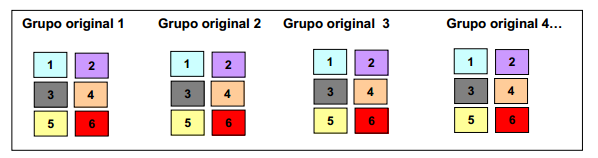
\includegraphics[scale=0.6]{figuras/jigsaw01}}\\
  \caption{Grupos originales en la técnica Jigsaw}\label{fig:jigsaw01}
\end{figure}

A los estudiantes con el número 1 se les reparte el mismo documento, que será diferente al resto de los compañeros y que puede corresponderse a la primera parte del tema de estudio. A los alumnos con el número 2 se les reparte otro documento y así sucesivamente.

La primera fase será, por tanto, que los alumnos preparen su documento de forma individual, que lo lean, que lo entienda, que lo aprendan y que recopilen las dudas que surjan.

  \item Una vez que ya ha finalizado el tiempo estimado para la preparación individual del documento, comienza la segunda fase que se denomina ``Reunión de expertos''. En este momento todos los alumnos con el mismo número se reúnen para debatir y comentar sobre el documento que les fue asignado. Ver figura \ref{fig:jigsaw02}

  \begin{figure}[h]
  \centering
  % Requires \usepackage{graphicx}
  \fbox{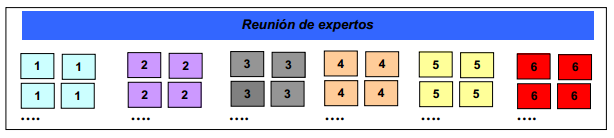
\includegraphics[scale=0.6]{figuras/jigsaw02}}\\
  \caption{Grupos de expertos}\label{fig:jigsaw02}
\end{figure}

    \item Finalizada las reuniones de expertos, llega la tercera fase, que supone el regreso al grupo original y, cada alumno explicará al resto de sus compañeros el documentos que ha estado preparando. Ver figura \ref{fig:jigsaw03}

\begin{figure}[h]
  \centering
  % Requires \usepackage{graphicx}
  \fbox{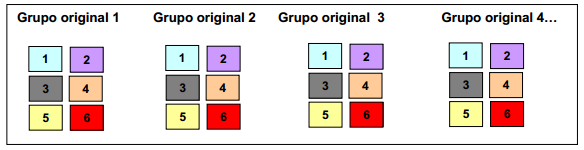
\includegraphics[scale=0.6]{figuras/jigsaw03}}\\
  \caption{Regreso a los originales}\label{fig:jigsaw03}
\end{figure}

\item La última fase, consiste en evaluar el aprendizaje logrado y la eficacia de la técnica individualmente. Para ello, el docente prepara un test sobre todo el material que ha sido trabajado durante la sesión de clase.

\end{enumerate}

\subsection{Programación en pares}
Una técnica educacional que tiene elementos en común con el aprendizaje cooperativo es la programación en pares. En esta forma de colaboración, dos programadores trabajan lado a lado en un computador. En cualquier momento, un miembro del equipo(``the driver'') está escribiendo en el computador o transcribiendo algún diseño elaborado. El otro integrante del equipo (``the navigator'') está observando activamente el trabajo del primero, buscando defectos, pensando en otras alternativas de solución, haciendo preguntas, etc. Los roles de ``driver'' y ``navigator'' son intercambiados periódicamente entre ambos miembros del equipo.\\

La programación en pares fue originalmente popularizada como parte de la metodología de desarrollo de software XP \cite{beck_extreme_2000}. Así mismo, resultados de investigaciones muestran que los programadores en pares producen código de mayor calidad en mitad de tiempo que lo programadores individuales \cite{williams2000collaborative,williams_strengthening_2000}. La técnica de programación en pares también ha mostrado ser efectiva para estudiantes de programación, logrando mejorar el aprendizaje en los alumnos\cite{mcdowell_effects_2002}.

%\subsection{El estudio de Casos}
%Es una técnica de aprendizaje cooperativo, la cual está basada en un enfoque de estudio de problemas. \cite{JCAL:JCAL119}. Durante un Estudio de Casos, los estudiantes reciben materiales que describen una situación en concreto y se les pide analizarla tratando de identificar los puntos fuertes y débiles del caso, así como también se les pide reflexionar sobre posibles soluciones que pudiesen añadir a las ya presentadas en el problema. El factor más importante del Estudio de Casos es que éstos están basados en problemas y/o situaciones reales \cite{JCAL:JCAL119}.
%

\section{Tecnologías web}


\subsection{AJAX}

El término AJAX es un acrónimo de Asynchronous JavaScript $+$ XML que puede traducirse como ``JavaScript asíncrono más XML''. El término AJAX se presentó por primera vez en el artículo ``Ajax, A new Approach to Web Applications" publicado por Jesse James Garret en el año 2005. En realidad, en dicho artículo se dice que AJAX no es una tecnología en sí misma sino un conjunto de varias tecnologías que se unen de formas nuevas y sorprendentes \cite{ajax_dummies_2006}.\\

AJAX está compuesto por los siguiente:

\begin{itemize}
  \item La presentación en el navegador está basada en HTML y CSS.
  \item Document Object Model (DOM), para la interacción y manipulación dinámica de la presentación.
  \item XML, XSLT y JSON, para el intercambio y la manipulación de información
  \item XMLHttpRequest, para el intercambio asíncrono de información.
  \item JavaScript, para unir todas las tecnologías antes mencionadas.
\end{itemize}
%Ver figura \ref{fig:ajax}
%\begin{figure}[h]
%  \centering
%  % Requires \usepackage{graphicx}
%  \fbox{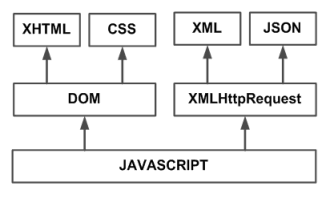
\includegraphics[scale=0.8]{figuras/ajax_01}}\\
%  \caption{Tecnologías agrupadas bajo el concepto de AJAX}\label{fig:ajax}
%\end{figure}

JavaScript es un lenguaje que la mayoría de navegadores soporta y que permite manipular datos entre la vista y el servidor. A continuación se indica cómo es que AJAX funciona:\cite{ajax_dummies_2006}

\begin{enumerate}
  \item En el navegador se escribe código en JavaScript con el cual se puede obtener información del servidor las veces que sean necesarias.
  \item Cuando más data es requerida, el JavaScript usa el objeto XMLHttpRequest para enviar la petición al servidor sin necesidad de refrescar toda la página web.
  \item La data que retorna desde el servidor puede estar en formato XML o puede ser sólo texto plano. Lo importante es que el JavaScript en el navegador puede leer la información recibida y mostrarla en la vista.
\end{enumerate}

\subsubsection{¿Qué se puede hacer con AJAX?}

AJAX ha estado presente desde 1998 y muchas aplicaciones como Microsoft's Outlook Web Access la han usado. Sin embargo, recien a partir del año 2005 cuando AJAX tomó sitio en el campo del desarrollo web después de que fuese utilizado en aplicaciones como Google Suggest y Google Maps.\cite{ajax_dummies_2006}\\

Desde entonces, AJAX ha permitido realizar diferentes tipos de aplicaciones web como por ejemplo:

\begin{itemize}
  \item \emph{Búsqueda en tiempo real}. Una de las mejores cosas que se puede realizar usando AJAX son las búsquedas en vivo, donde el usuario obtiene lo que busca mientras va escribiendo lo que necesita buscar.
  \item \emph{Obtener la respuesta con autocompletado}. Muy parecido a las búsquedas en vivo son las aplicaciones que tratan de adivinar la palabra que estamos escribiendo obteniendo una lista de palabras similares del servidor que son puestas a nuetra vista.
  \item \emph{Chatear con amigos}. Puesto que AJAX no necesita refrescar toda la página web, es una buena herramienta para realizar programas de chat donde muchos usuarios conversan al mismo tiempo.
  \item \emph{Dragging and Dropping}.
  \item \emph{Juegos con AJAX}.
  \item \emph{Menús pop up}. Se puede obtener data desde el servidor tan pronto como sea necesario usando Ajax.
\end{itemize}

\subsection{Polling}
Después del posicionamiento de AJAX, no pasó mucho tiempo para tratar de lograr que los eventos en el navegador salieran fuera de la ecuación y se pudiera automatizar el proceso de obtener nueva información desde el servidor. Fue entonces que los desarrolladores establecieron un intervalo de actualización para revisar actualizaciones cada $n$ segundos \cite{lengstorf_realtime_2013}. Ver figura \ref{fig:polling}

\begin{figure}[!h]
  \centering
  % Requires \usepackage{graphicx}
  \caption{Polling}{A través del Polling se envía peticiones HTTP para comprobar si existe nueva información.}
  \fbox{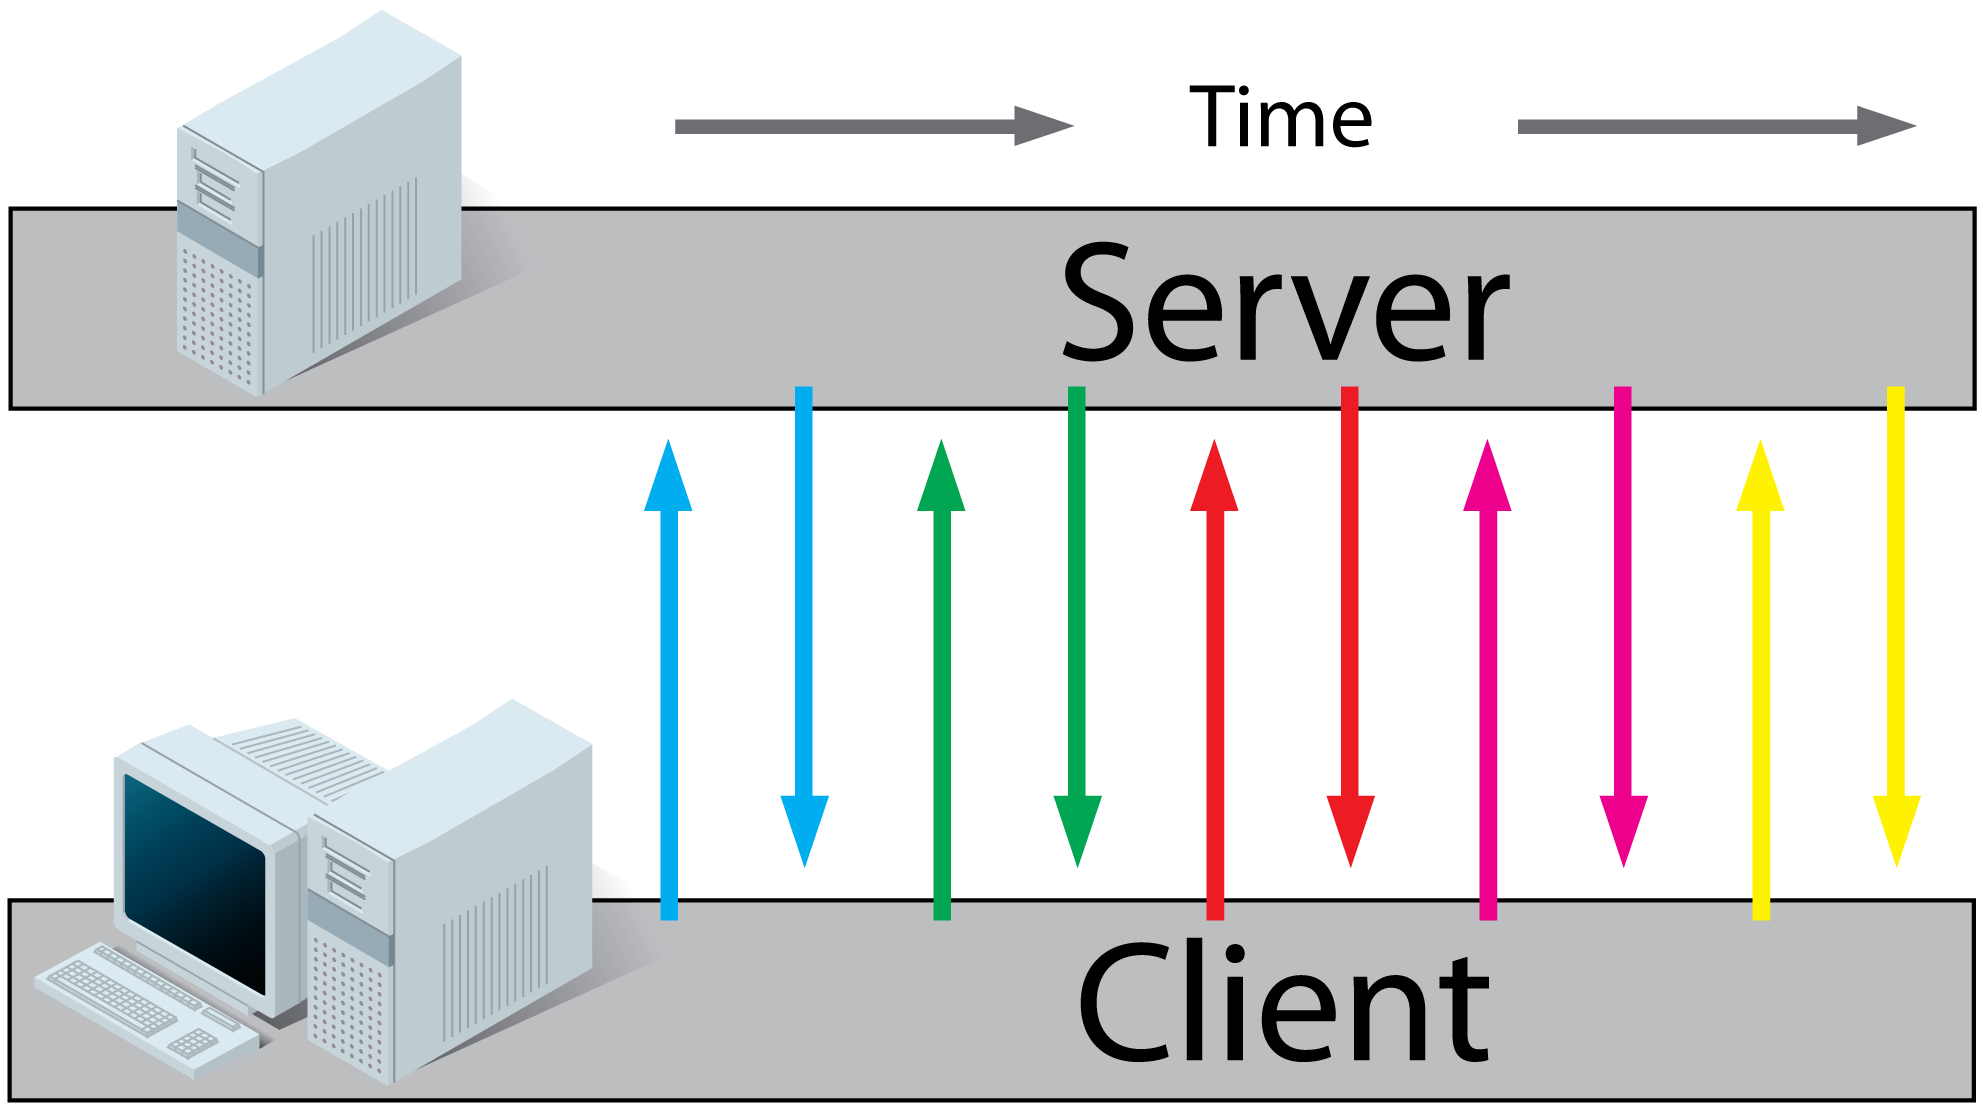
\includegraphics[scale=0.6]{figuras/ajax_polling}}\\
  \label{fig:polling}
  \source {\citeNP {lengstorf_realtime_2013}}
\end{figure}

\subsection{HTTP Long-Polling}
El siguiente paso en la evolución del tiempo real es el HTTP \emph{long-polling}, el cual consiste en abrir una petición HTTP por un periodo de tiempo para escuchar respuestas del servidor. Si hubiese nueva data, el servidor la enviaría y se cerraría la petición; de otro modo, la petición es cerrada después de un intervalo de tiempo límite y se abre una nueva petición \cite{lengstorf_realtime_2013}.  Ver figura \ref{fig:http_long_polling}
\begin{figure}[h]
  \centering
  % Requires \usepackage{graphicx}
  \caption{Long Polling}{Gracias al HTTP Long-polling, se mantiene abierta una peticion HTTP por un periodo de tiempo para comprobar si existe nueva información.}
  \label{fig:http_long_polling}  
  \fbox{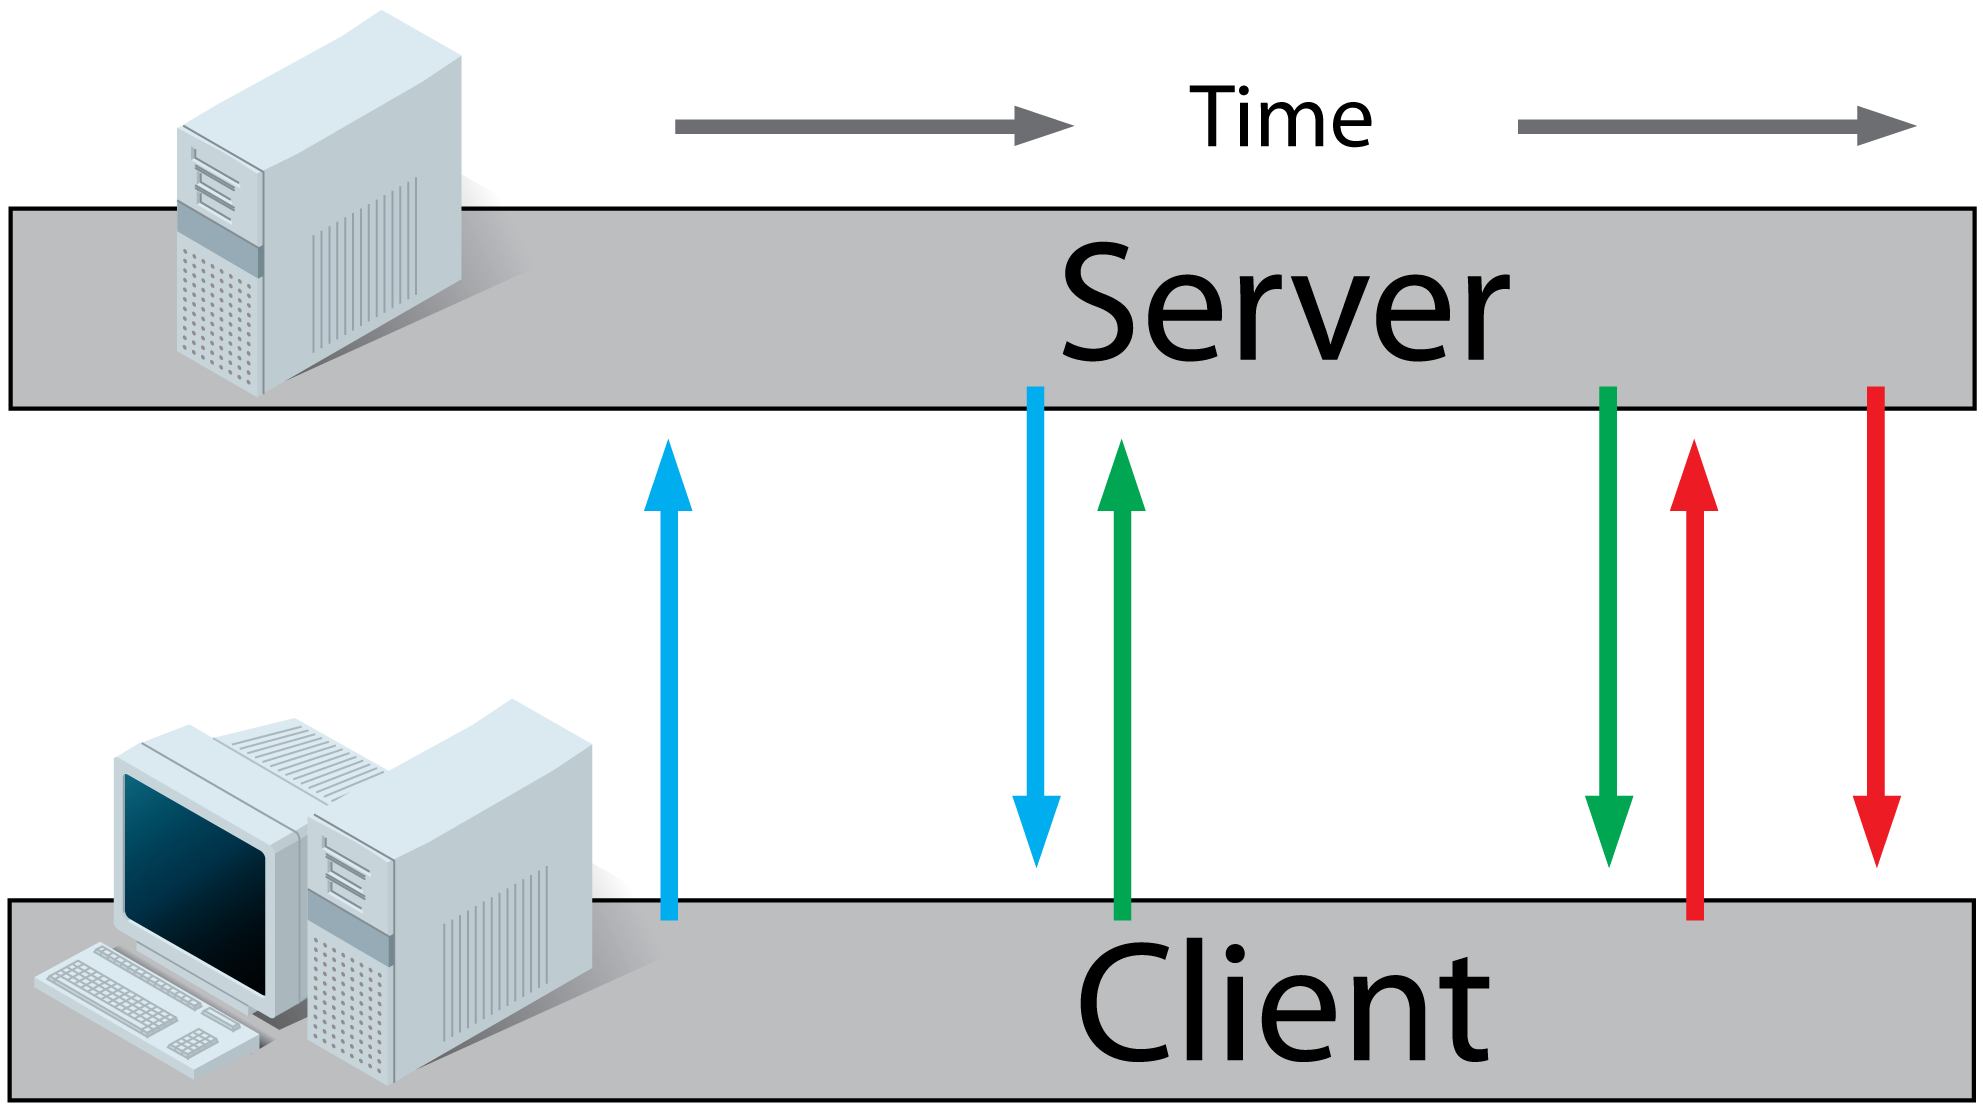
\includegraphics[scale=0.6]{figuras/ajax_long_polling}}\\
    \source {\citeNP {lengstorf_realtime_2013}}
\end{figure}
%%\cite{lengstorf2013realtime}

\subsection{WebSockets}
Web sockets (Ver figura \ref{fig:websockets}) es una tecnología que proporciona un canal de comunicación bidireccional y full-duplex sobre una única conexión TCP en los navegadores y servidores web. A comparación de HTTP, WebSocket puede reducir efectivamente el tráfico de red innecesario, a través de una forma estandarizada para que el servidor envíe contenido al navegador sin que éste sea solicitado.\cite{cheng_new_2013}\\

\begin{figure}[h]
  \centering
  % Requires \usepackage{graphicx}

  \caption{Websockets}{Una nueva tecnología para la comunicación bidireccional.}
    \fbox{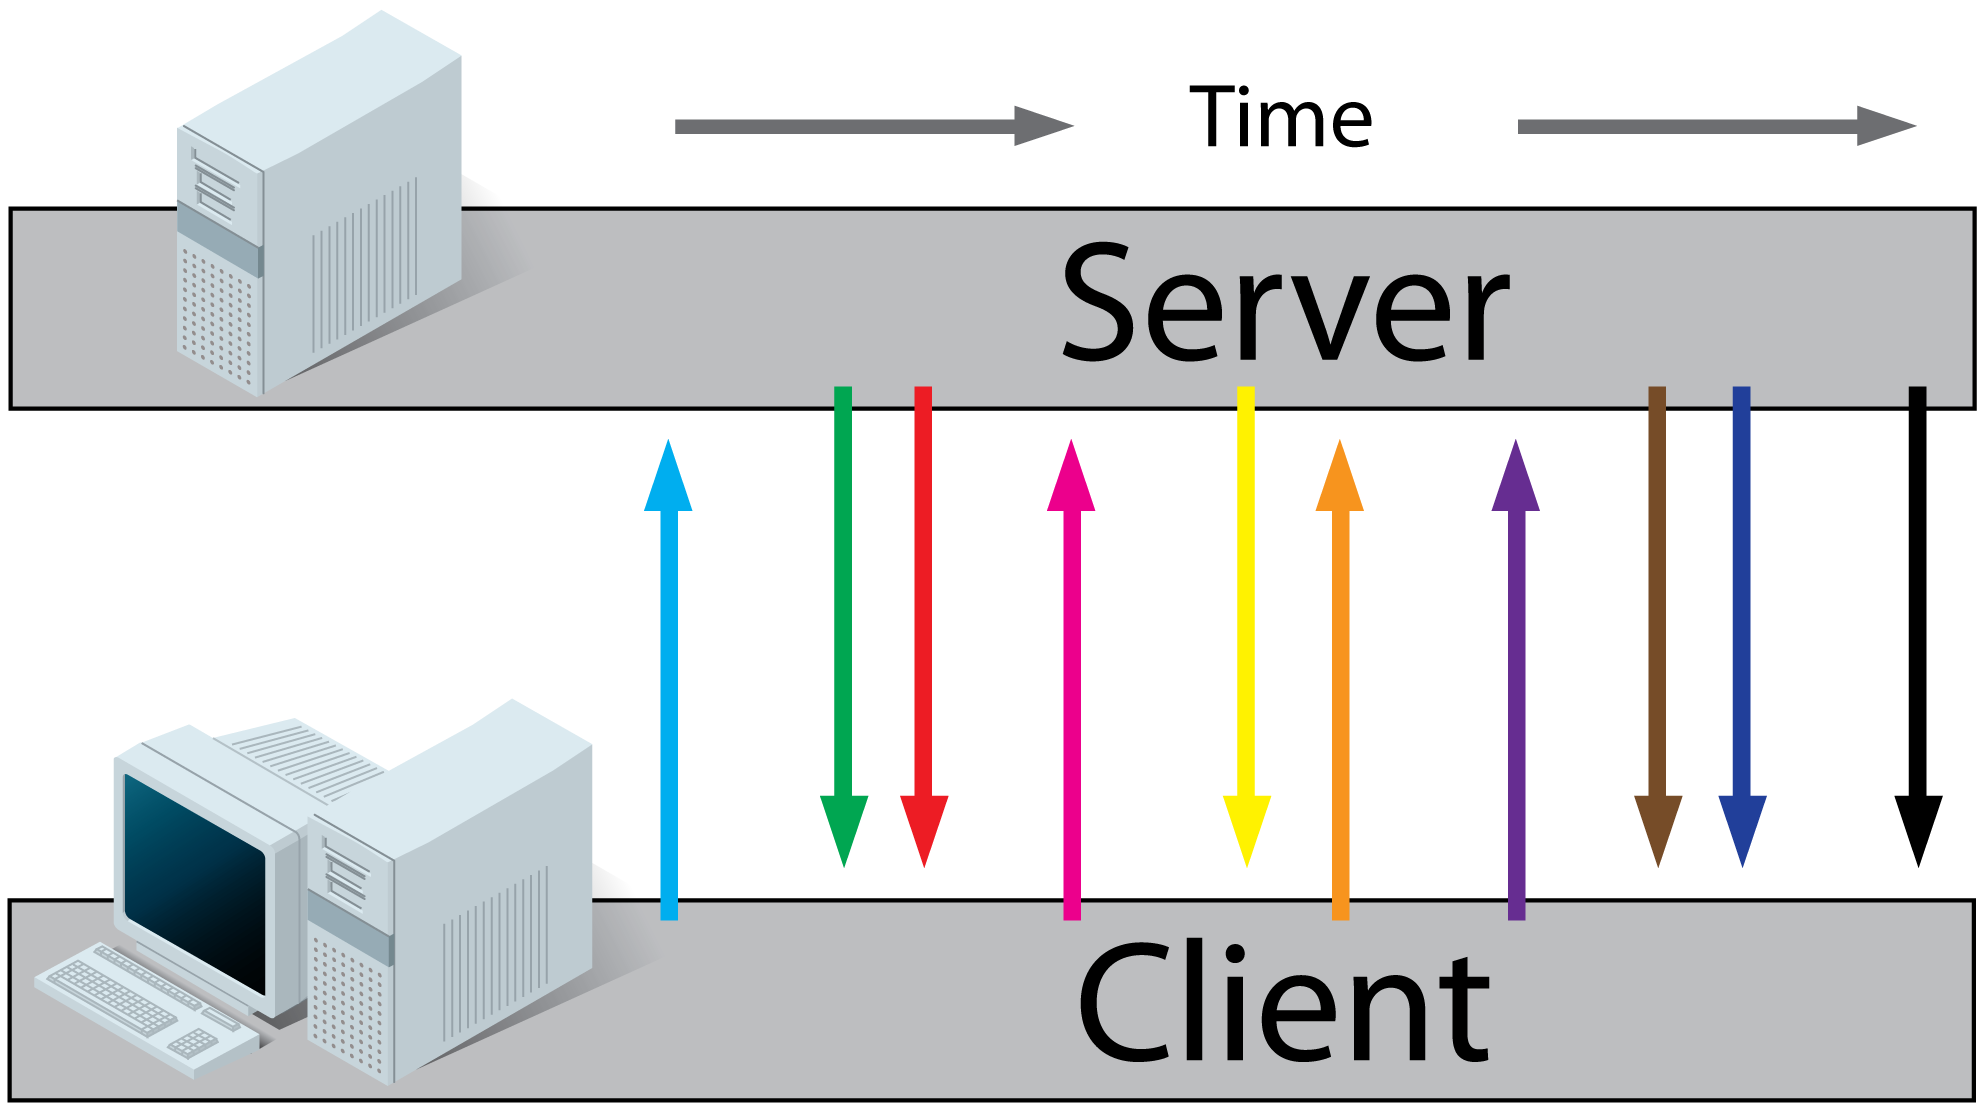
\includegraphics[scale=0.6]{figuras/websockets}}\\
    \source {\citeNP {lengstorf_realtime_2013}}
  \label{fig:websockets}
\end{figure}

\subsubsection{¿Por qué usar Websockets?}

Existen muchas razones que no conllevan a utilizar websockets cuando desarrollemos una aplicación web. Algunas de ellas se mencionan a continuación:

\begin{itemize}
  \item Websockets permite que la comunicación en tiempo real sea mucho más eficiente. Desde luego, siempre será posible usar polling sobre HTTP para recibir las notificaciones desde el servidor. Sin embargo, con el uso de Websockets se ahorra ancho de banda, cpu, y latencia.
  \item La comunicación entre el cliente y el servidor se vuelve más sencilla.
\end{itemize}

Los websockets tiene una gran acogida de parte de la comunidad de desarrolladores, lo cual se ve reflejado en la variedad de implementaciones de websockets como Apache mod\_pywebsocket, Jetty, Socket.IO, entre otros.


\section{Glosario}

\begin{enumerate}
  \item \textbf{Framework}. La palabra inglesa "framework" (marco de trabajo) define, en términos generales, un conjunto estandarizado de conceptos, prácticas y criterios para enfocar un tipo de problemática particular que sirve como referencia, para enfrentar y resolver nuevos problemas de índole similar.
  \item \textbf{Librería}. En informática, una librería es un conjunto de implementaciones funcionales, codificadas en un lenguaje de programación, que ofrece una interfaz bien definida para la funcionalidad que se invoca.
  \item \textbf{Socket}. Designa un concepto abstracto por el cual dos programas (posiblemente situados en computadoras distintas) pueden intercambiar cualquier flujo de datos, generalmente de manera fiable y ordenada.
%  \item \textbf{Tiempo real}. Un sistema en tiempo real (STR) es aquel sistema digital que interactúa activamente con un entorno con dinámica conocida en relación con sus entradas, salidas y restricciones temporales, para darle un correcto funcionamiento de acuerdo con los conceptos de predictibilidad, estabilidad, controlabilidad y alcanzabilidad
  \item \textbf{CSCL}. Computer-Supported Collaborative Learning. Aprendizaje colaborativo apoyado por computador.
  \item \textbf{API}. Application Programming Interface. Es el conjunto de funciones y procedimientos que ofrece cierta librería para ser utilizado por otro software como un capa de abstracción. Representa la capacidad de comunicación entre componentes de un software.
\end{enumerate}














\chapter{Estado del Arte}
\label{cap:estado_del_arte}
En este capítulo se desarrollo el estado del arte de las herramientas para el aprendizaje colaborativo como son LearnCS, GoogleDocs, entre otros, las mismas que son analizadas en un cuadro comparativo. Además, también se describe el estado del arte de 2 técnicas de aprendizaje colaborativo que serán usadas para la presente tesis. Finalmente, se desarrolla el estado del arte de algunos frameworks y APIs que serán utilizadas para la implementación del sistema web para el aprendizaje colaborativo.

\section{Herramientas para el aprendizaje colaborativo}

\subsection{LearnCS}
\emph{LearnCS!} es un entorno de programación creado específicamente para el uso de estudiantes de primer año de la carrera de ciencias de la computación. Este programa elimina la necesidad de los alumnos de tener que preocuparse por un editor de texto, comandos linux y proceso de compilación. LearnCS! proveee un entorno web en el cual los alumno pueden escribir, ejecutar y depurar programas usando un interfaz familiar y amigable. El compilador de C embebido que posee el sistema permite al alumno ejecutar sus programas con simplemente hacer click en un botón y obtener los resultados de ejecución de su código fuente \cite{lipman_learncs_2014}.\\

En muchos cursos de programación de primer ciclo, el concepto de depurar un programa es enseñado a finales del curso. En cambio, a través de \emph{LearnCS!}, los alumnos pueden establecer puntos de corte en el programa y empezar a depurar paso a paso su código fuente. Además, el sistema brinda la opción de ver la representación de la memoria y así visualizar en detalle el estado de su programa. Cuando se llaman a funciones, los alumnos aprenden cómo los argumentos y variables locales son colocados en la pila de la memoria y cómo las variables son reservadas en memoria \cite{lipman_learncs_2014}.\\

\begin{figure}[!h]
  \centering
  % Requires \usepackage{graphicx}
  \fbox{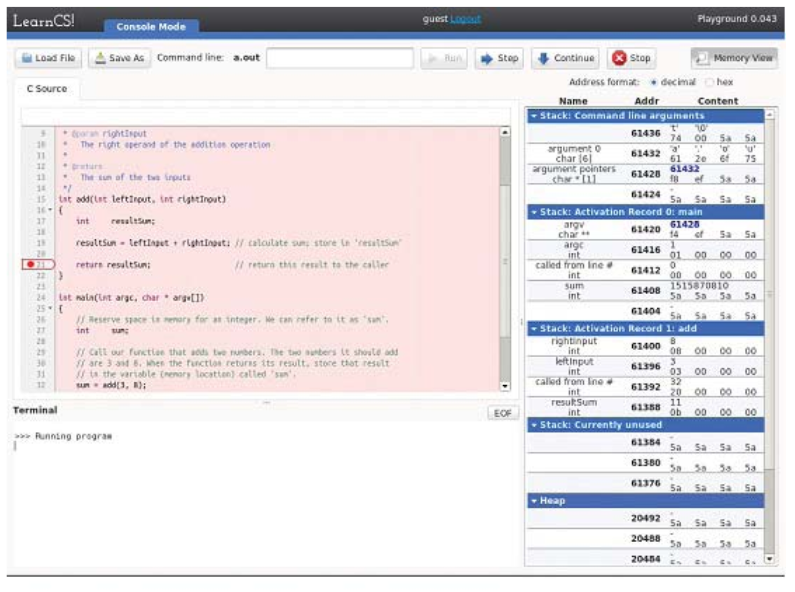
\includegraphics[scale=0.4]{figuras/learncs.png}}\\
  \caption[LearnCS]{Interfaz del sistema LearnCS! \protect\cite{lipman_learncs_2014}}
  \label{fig:learncs}
\end{figure}

LearnCS! fue creado para proporcionar un ambiente de aprendizaje para estudiantes de informática de primer año. Sus principales objetivos son proporcionar asistencia útil al alumno en la construcción de un modelo mental de la máquina nocional de C a través de la visualización detallada de la memoria de \emph{LearnCS!} y sus mensajes de error integrados en las instalaciones de depuración, y para proporcionar que producen consejos que son útiles para el principiante para localizar y corregir errores de sintaxis\cite{lipman_learncs_2014}.\\

LearnCS! se ejecuta en un navegador web y tal como se muesta en la Figura \ref{fig:learncs}, ofrece lo siguiente:

\begin{enumerate}
  \item (Panel superior-izquierdo) Un área de la pantalla dedicada a la edición del programa que se está desarrollando.
  \item (Panel derecho) Una representación de la vista de la memoria.
  \item (Panel inferior) Una zona de ``salida'' que contiene una ``terminal'' para la entrada y salida de texto.
  \item (Panel inferior-derecho) Opcionalmente, como se muestra en la figura \ref{fig:learncs2}, se muestra un área gráfica que permite desarrollar programas más interactivos y más interesantes para los alumnos.
\end{enumerate}

\begin{figure}[!h]
  \centering
  % Requires \usepackage{graphicx}
  \fbox{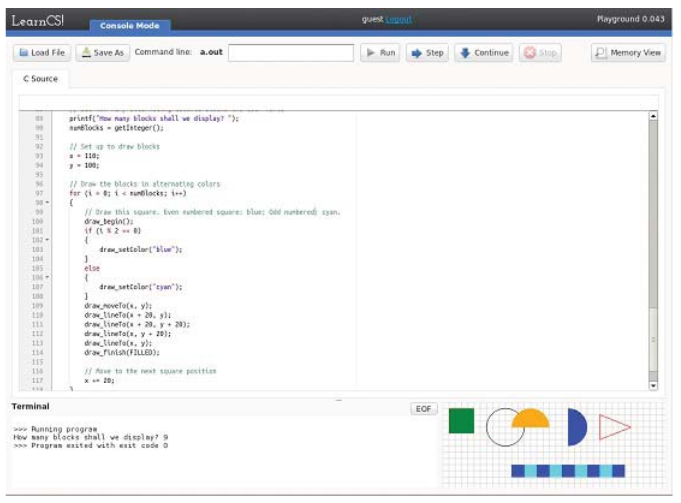
\includegraphics[scale=0.5]{figuras/learncs2.png}}\\
  \caption[LearnCS]{Área gráfica para programas más interactivos en LearnCS! \protect\cite{lipman_learncs_2014}}\label{fig:learncs2}
\end{figure}

\subsection{Google Docs}

Google Docs es un conjunto de herramientas online que permiten elaborar documentos, hojas de cálculo, dibujos y diapositivas de manera colaborativa usando solamente un navegador web. Esta herramienta es un gestor de documentos pues a través de ella se pueden subir a la nube todo tipo de archivos y ordenarlos en carpetas así como compartirlos con otros usuarios \cite{googledocs}.\\

Para acceder a esta herramienta de colaboración, en primer lugar se debe tener una cuenta de gmail y con ello se obtiene el acceso a Google Docs a través del siguiente link \url{http://docs.google.com/}. Las funcionalidades más resaltantes que posee GoogleDocs son las siguientes: \cite{googledocs}\\

\begin{enumerate}
  \item \emph{Crear documentos básicos desde cero}. Con GoogleDocs es posible realizar tareas que corresponden al manejo de documentos de oficina, como crear documentos de texto, hojas de cálculo, presentaciones de diapositivas, y añadirles a todos ellos imágenes, comentarios o fórmulas, entre otras muchas cosas más.
  \item \emph{Subir archivos ya creados}. Existe la opción de subir archivos que ya están creados y para ellos, Google Docs acepta la mayoría de formatos de archivos comunes como DOC, XLS, ODT, CSV, PPT, PDF, etc.
  \item \emph{Editar un documento}. GoogleDocs posee una barra de herramientas que nos permite aplicar negrita, subrayar, cambiar la fuente, color, etc.
  \item \emph{Compartir documentos.} Cuando se edita un documento, existe la opción de invitar a otros usuarios, enviar el documento por correo electrónico, publicarlo como página web, ver quién tiene acceso, etc.
  \item \emph{Chatear en tiempo real con otros usuarios}.
  \item \emph{Exportar documentos}. Google Docs permite descargar nuestros documentos en el escritorio en archivos Word, Excel, OpenOffice, RTF, PDF, HTML o ZIP.
\end{enumerate}
%A continuación se detalla qué es posible realizar con los documentos, hojas de cálculo y presentaciones que GoogleDocs nos permite elaborar de forma colaborativa.\\

%\textbf{DOCUMENTOS}\\
%
%\begin{itemize}
%  \item Subir documentos de Word, OpenOffice, RTF, HTML o texto (o crear documentos desde cero).
%  \item Invitar a otros usuarios (por su dirección de correo electrónico) para que puedan editar o ver los documentos.
%  \item Editar documentos on line en forma colaborativa con otras personas.
%  \item Ver el historial de revisiones de nuestros documentos y hojas de cálculo y volver a cualquier versión.
%  \item Publicar documentos on line para que estén disponibles para todo el mundo.
%  \item Descargar documentos en el escritorio como documentos de Word, de OpenOffice, RTF, PDF, HTML o ZIP.
%  \item Enviar por correo electrónico los documentos como archivos adjuntos.
%  \item Chatear en tiempo real con otros usuarios.
%\end{itemize}
%
%\textbf{HOJAS DE CÁLCULO}\\
%
%\begin{itemize}
%  \item Importar y exportar datos con los formatos .xls, .csv y .ods
%  \item Usar la edición de formatos y fórmulas en las hojas de cálculo, con lo que podremos calcular resultados y dar a los datos el aspecto que deseemos.
%  \item Chatear en tiempo real con otros usuarios.
%  \item
%  \item
%
%\end{itemize}

\begin{figure}[!h]
  \centering
  % Requires \usepackage{graphicx}
  \fbox{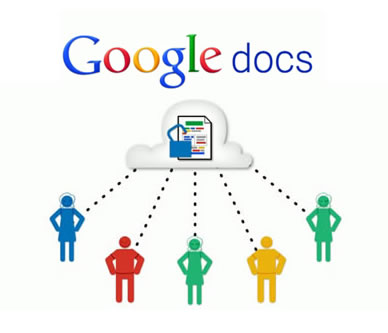
\includegraphics[scale=0.8]{figuras/googledocs.jpg}}\\
  \caption[Google Docs]{GoogleDocs \protect\cite{googledocs}}\label{fig:googledocs}
\end{figure}

\clearpage
\subsection{Sistema Web para la enseñanza de Casos
de Uso empleando la Técnica de Aprendizaje Cooperativo
de Rompecabezas.}

Este sistema es producto de una tesis de grado implementada en la Pontificia Universidad Católica del Perú. El sistema pretende dar soporte a las tres fases que comprende una clase en la cual se emplea la técnica de Jigsaw para lo cual, se construyeron los módulos de Planificación, Ejecución y Evaluación.\\

El módulo de Planificación permite realizar el diseño de cada sesión de clase. Ahí se plantean los datos de la sesión que serán la base de los objetivos y resultados esperados que permitirán medir el progreso académico de los alumnos.\\

El módulo de Ejecución se encarga de llevar a cabo la ejecución de una sesión de clase basada en la técnica de Jigsaw. Permite el desarrollo paso a paso desde la lectura de materiales, documentos y casos hasta la diagramación de la solución que brinden cada uno de los grupos Jigsaw y Expertos. En este módulo se cuenta con foros de discusión que permiten la comunicación entre los miembros de cada grupo.\\

Por último se tiene el módulo de Evaluación, en el cual se elaboran preguntas y examenes que luego el profesor aplica a sus alumnos. Estos exámenes son calificados manualmente o de forma automática por el propio sistema.

%\subsubsection{ARQUITECTURA DEL SISTEMA}

El sistema fue desarrollado usando una arquitectura Modelo-Vista-Controlador. Se usó Java como plataforma de desarrollo y MySQL como motor de base de datos. Acontinuación se indican los frameworks utilizados en el sistema:

\begin{itemize}
  \item Framework J2EE
  \item Struts 2
  \item MyBatis
  \item Librerías AJAX: JQuery, DojoToolKit
\end{itemize}

El sistema desarrollado consta de 3 módulos que se detallan a continuación:\\

\textbf{Planificación}\\

Este módulo posee las siguientes funcionalidades:
\begin{enumerate}
  \item Crear dinámica de Curso
  \item Consultar información del curso
  \item Consultar configuración de dinámica
  \item Consultar información de dinámica
  \item Actualizar mensaje interno
\end{enumerate}

\textbf{Ejecución}\\

Este módulo se encarga de llevar a cabo el desarrollo de una sesión basada en la técnica de aprendizaje colaborativo de rompecabezas. Permite la lectura de materiales y documentes, hasta la elaboración colaborativa de la solución a los diferentes problemas propuestos en los diferentes grupos Jigsaw y Expertos.\\

El módulo cuenta con herramientas de chat para la comunicación online, así como también de un foro para la discusión de los temas.\\

Este módulo posee las siguientes funcionalidades:

\begin{enumerate}
  \item Actualizar publicación en foro
  \item Ingresar sesión cooperativa
  \item Controlar estado de la dinámica
  \item Elaborar casos de uso,.
\end{enumerate}

\textbf{Evaluación}\\

En esta parte del sistema es donde se elaboran las preguntas y exámenes por parte del docente y posteriormente se aplican a los alumnos. El sistema permite que estos exámenes sean evaluados manualmente o de forma automática.

Este módulo posee las siguientes funcionalidades:
\begin{enumerate}
  \item Consultar configuración de evaluación.
  \item Consultar corrección de evaluación.
  \item Consultar calificación de evaluación.
  \item Crear evaluación.
  \item Rendir evaluación.
  \item Realizar calificación.
\end{enumerate}


\emph{Fuente} \cite{pinzas_desarrollo_2013}

\subsection{CodeBunk}
\begin{figure}[h]
  \centering
  % Requires \usepackage{graphicx}
  \fbox{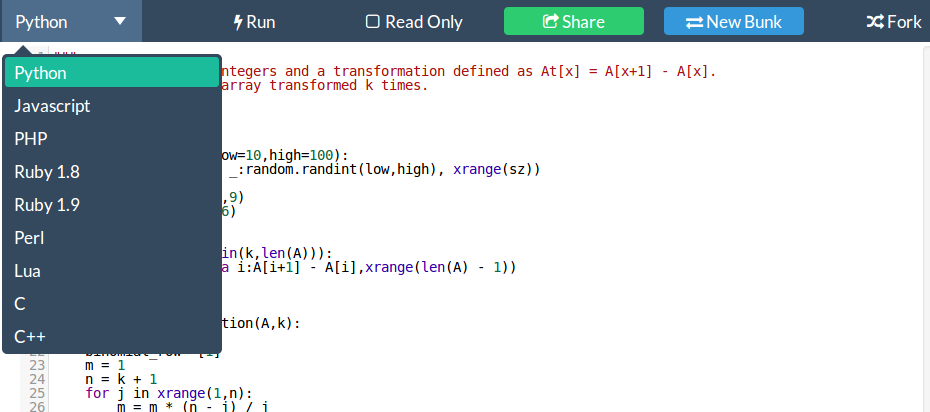
\includegraphics[scale=0.3]{figuras/codebunk.png}}\\
  \caption[CodeBunk]{Interfaz gráfica de Codebunk \protect\cite{codebunk}}\label{fig:codebunk}
\end{figure}
Es una plataforma que permite codificar y compilar en diferentes lenguajes de programación de forma colaborativa y en tiempo real. Algunas de sus funcionalidades son las siguientes:\\

\begin{enumerate}
  \item Posee un editor colaborativo que soporta 14 lenguajes de programación, tiene coloración de sintaxis según el lenguaje y brinda un indentado inteligente.
  \item Compilar y Ejecutar. La plataforma permite compilar y ejecutar código en Python, Java, C, C++, Ruby, Javascript, entre otros.
  \item Audio y Video Chat.
  \item Code playback. Permite repetir la historia de los cambios realizados en el código.
  \item Equipos. Permite crear equipos de trabajo e invitar a otros usuarios a colaborar en el desarrollo de un programa.
\end{enumerate}


\newpage
\subsection{Análisis comparativo}
Las cuatro herramientas para el aprendizaje colaborativo que se han estudiado hasta el momento son resumidas y comparadas en el siguiente cuadro, en el cual se podrá apreciar las características que nos ofrece cada una de las cuatro aplicaciones presentadas anteriormente.\\
%\begin{landscape}
\begin{longtable}{|L{7cm}|C{1.5cm}|C{1.5cm}|C{1.5cm}|C{1.5cm}|}
\caption{Herramientas para el aprendizaje colaborativo}
\label{tab:herramientasAC}\\
    \toprule[0.8mm]
    CARACTERÍSTICAS	& LearnCS &	Google Docs & Sistema PUCP & Code Bunk\\	
    \midrule[0.6mm]
    $\diamond$ Permite desarrollar código fuente &\cmark	&\xmark	&\xmark	&\cmark	\\
    $\diamond$ Permite desarrollar código fuente de forma colaborativa	&\xmark	&\xmark	&\xmark	&\cmark	\\
    $\diamond$ Posee un representación de la memoria del computador	&\cmark	&\xmark	&\xmark	&\xmark	\\
    $\diamond$ Muestra mensajes de error	&\cmark	&\xmark	&\xmark	&\cmark	\\
    %$\diamond$ Brinda coloreado de sintaxis de lenguaje C	&\cmark	&\xmark	&\xmark	&\cmark	\\
%    $\diamond$ Es un aplicativo web	&\cmark	&\cmark	&\cmark	&\cmark	\\
    %$\diamond$ Soporta sólamente lenguage C	&\cmark	&\xmark	&\xmark	&\xmark	\\
    $\diamond$ Permite crear y editar documentos de texto, hojas de cálculo y diapositivas &\xmark	&\cmark	&\xmark	&\xmark	\\
    %$\diamond$ Subir archivos ya creados	&\xmark	&\cmark	&\xmark	&\xmark	\\
    %$\diamond$ Edición de documentos de texto	&\xmark	&\cmark	&\cmark	&\cmark	\\
%    $\diamond$ Permite crear y editar hojas de cálculo	&\xmark	&\cmark	&\xmark	&\xmark	\\
%    $\diamond$ Permite crear y editar diapositivas	&\xmark	&\cmark	&\xmark	&\xmark	\\
    $\diamond$ Permite compartir documentos con otros usuarios	&\xmark	&\cmark	&\xmark	&\cmark	\\
    $\diamond$ Permite la comunicación a través de un Chat	&\xmark	&\cmark	&\xmark	&\cmark	\\
    %$\diamond$ Exportar documentos 	&\xmark	&\cmark	&\xmark	&\xmark	\\
    $\diamond$ Permite diseñar una sesión de clase jigsaw	&\xmark	&\xmark	&\cmark	&\xmark	\\
    $\diamond$ Permite tomar y calificar evaluaciones	&\xmark	&\xmark	&\cmark	&\xmark	\\
    $\diamond$ Permite la comunicación a través de un foro de discusión	&\xmark	&\cmark	&\cmark	&\xmark	\\
    $\diamond$ Permite elaborar casos de uso	&\xmark	&\xmark	&\cmark	&\xmark	\\
   
    %$\diamond$ Java, Python, C, C++, etc	&\xmark	&\xmark	&\xmark	&\cmark	\\
    $\diamond$ Posee coloración de sintaxis de código fuente	&\cmark	&\xmark	&\xmark	&\cmark	\\
%    $\diamond$ Indentado inteligente	&\xmark	&\xmark	&\xmark	&\cmark	\\
    %$\diamond$ Compilar y ejecutar de código fuente	&\xmark	&\xmark	&\xmark	&\cmark	\\
    %$\diamond$ Ejecución de código fuente	&\xmark	&\xmark	&\xmark	&\cmark	\\
    $\diamond$ Visualización de resultados de ejecución	&\xmark	&\xmark	&\xmark	&\cmark	\\
    $\diamond$ Historial de revisiones de código	&\xmark	&\cmark	&\xmark	&\cmark	\\
    $\diamond$ Creación de equipos colaborativos	&\xmark	&\cmark	&\xmark	&\cmark	\\
%    $\diamond$ Juez virtual de programación	&\xmark	&\xmark	&\xmark	&\xmark	\\
    $\diamond$ Posee un banco de preguntas de programación	&\xmark	&\xmark	&\xmark	&\xmark	\\
    \bottomrule[0.8mm]
\end{longtable}
%\end{landscape}
\newpage
\section{Técnicas para el aprendizaje colaborativo}

\subsection{Jigsaw}
Jigsaw es una técnica de aprendizaje colaborativo y recientemente ha sido aplicada por \citeA{Buhr2014429} a un grupo de estudiantes de medicina  de la Universidad de Duke tal y como se describe en el artículo \emph{``Using the Jigsaw Cooperative Learning Method to Teach Medical Students About Long Term and Postacute Care''}. En este estudio se desarrolló una experiencia colaborativa usando la técnica de Jigsaw para exponer a los estudiantes sobre el cuidado intensivo a largo plazo  (LTPAC - Long Term and Post Acute Care) y así lograr que ellos conozcan las herramientas y roles del personal involucrado en este tipo de cuidados de pacientes en un asilo de ancianos. Para alcanzar este objetivo, pequeños grupos de estudiantes de medicina realizaron entrevistas al personal de LTPAC sobre sus respectivos roles. Estos grupos posteriormente fueron reorganizados en nuevos grupos conteniendo un estudiante de cada grupo original más un moderador y cada estudiante en los nuevos grupos tuvo que explicar sobre el rol del profesional LTPAC al cual había entrevistado \cite{Buhr2014429}.\\

\begin{figure}[!h]
  \centering
  % Requires \usepackage{graphicx}
  \fbox{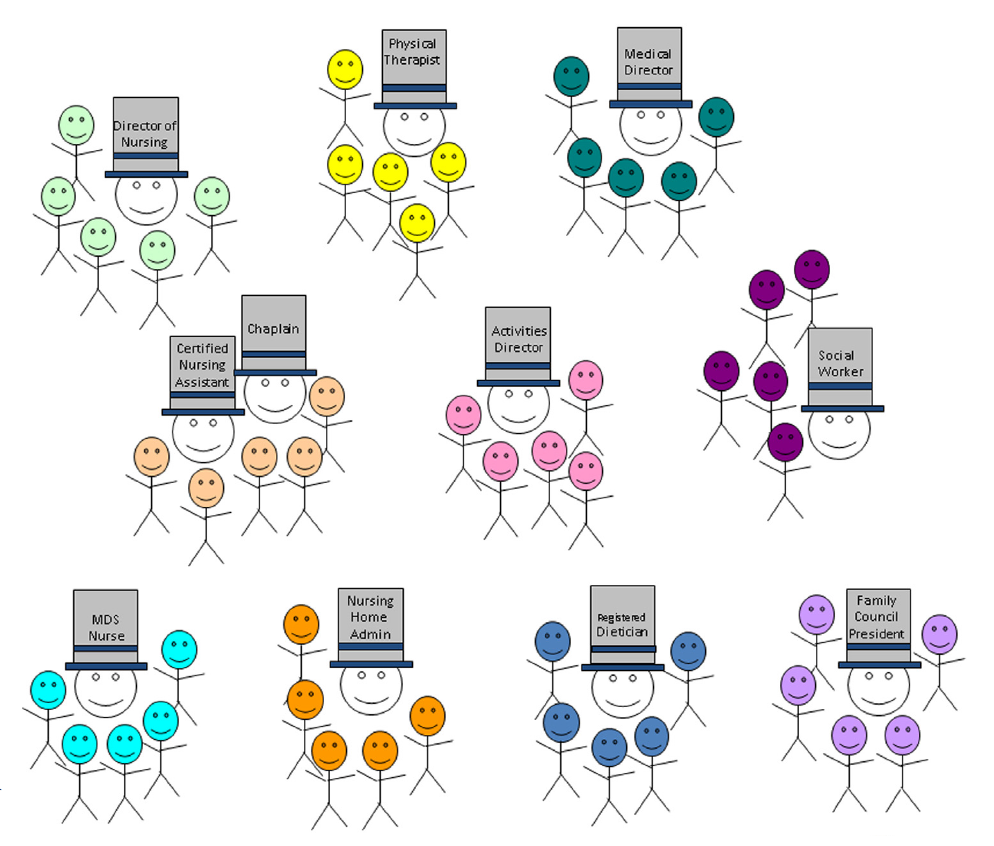
\includegraphics[scale=0.3]{figuras/jigsaw_ltpac_1.png}}\\
  \caption{Jigsaw Paso 1}{Fase de reunión de grupos de expertos \protect\cite{Buhr2014429} }
  \label{fig:jigsaw_ltpac_1}
\end{figure}

Los objetivos del ejercicio jigsaw realizado fueron para definir LTPAC, identificar cuáles son los alcances de este tipo de servicios que se brindan a los pacientes y describir los roles de los miembros del equipo que laboraba en el asilo de ancianos. Para esto, 10 miembros claves del equipo LTPAC fueron identificados y un total de 50 estudiantes fueron divididos en 10 grupos expertos. A cada grupo experto le fue asignado de 30 a 45 minutos para encontrar y entrevistar a 1 miembro del equipo LTPAC(Ver figura \ref{fig:jigsaw_ltpac_1}). Cada estudiante en el grupo tenía que convertirse en un experto sobre el rol del miembro que le fue asignado. Después de las entrevistas, los estudiantes tuvieron un tiempo de 15 minutos para debatir en sus grupos de expertos sobre los aspectos más resaltantes del rol del profesional al que entrevistaron. Finalmente, los grupos fueron reorganizados conteniendo un estudiante experto de cada grupo original así como un moderador(Ver figura \ref{fig:jigsaw_ltpac_2}). Lo nuevos grupos Jigsaw se reunieron por 1 hora durante la cual cada estudiante expuso los resultados de la entrevista que había realizado al profesional LTPAC del asilo \cite{Buhr2014429}.\\

\begin{figure}[!h]
  \centering
  % Requires \usepackage{graphicx}
  \fbox{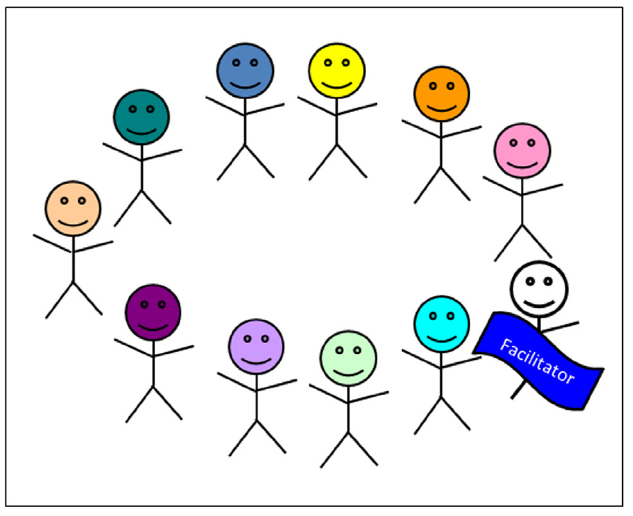
\includegraphics[scale=0.5]{figuras/jigsaw_ltpac_2.png}}\\
  \caption{Jigsaw Paso 2}{Fase de reunión de grupos Jigsaw dirigidos por un moderador \protect\cite{Buhr2014429} }
  \label{fig:jigsaw_ltpac_2}
\end{figure}

La efectividad de esta experiencia de aprendizaje fue medida a través de los comentarios por escrito de los estudiantes y el personal LTPAC así como también a través de una encuesta con una escala de 5 puntos donde 1 reflejaba malo y 5 significaba bueno. Los estudiantes también fueron evaluados con un examen de conocimientos sobre el tema tratado en la actividad desarrollada en el asilo. Los resultados de este examen indicaron que los estudiantes aprendieron los roles del personal LTPAC de forma satisfactoria. En general, el ejercicio jigsaw fue bien recibido por todos los participantes y mostró ser un medio eficaz para introducir a los estudiantes de medicina en el mundo del cuidado de ancianos \cite{Buhr2014429}.\\

\subsection{Pair Research}
En el estudio \emph{``Pair Research: Matching People for Colaboration, Learning, and Productivity''} elaborado por \citeA{miller_pair_2014} se describe una nueva forma de interacción denominada \emph{``Pair Research (Investigación en pares)''} que permite incrementar la productividad, el aprendizaje y la colaboración entre los diferentes grupos de investigación. A lo largo del artículo, los autores detallan un forma de cómo elaborar los grupos y además presentan los resultados obtenidos, los cuales mostraron que los miembros de los equipos usaban la investigación en pares en diferentes maneras incluyendo programación en pares, lluvia de ideas, recolección de data y análisis.\\

Pair Research es una generalización de la programación en pares. Cada semana, los miembros de los grupos son emparejados guidados por algoritmo de emparejamiento. Cada pareja se reune por una a dos horas de las cuales la mitad del tiempo es dedicado a trabajar en el proyecto de la otra persona. El trabajo puede ser cualquier actividad relacionada a programación, pruebas, diseño, recolección de datos y análisis, lluvia de ideas y asesoría. La siguiente semana, se forman nuevas parejas y el proceso se repite.\\

\citeA{miller_pair_2014} elaboraron un prototipo de hoja de cálculo para gestionar la investigación en pares de tal forma que cada semana, el sistema automáticamente hacía recordar a los miembros del grupo que envíen en qué necesitaban ayuda y en qué aspecto cada uno podía ayudar al resto para luego realizar el respectivo emparejamiento y notificar a cada miembro quien sería su siguiente pareja. Lo principal del prototipo elaborado (Ver figura \ref{fig:pair_research}) es la matriz de preferencias para el emparejamiento de personas. Cada semana, los miembros de cada grupo especificaban la ayuda que necesitaban en esa semana como por ejemplo: ``depurar programa en Django'' o ``revisar un informe''. Otros miembros luego completaban la matriz de preferencias de acuerdo a si podían o estaban interesados en ayudar en algún tema en específico; Para esto, ellos tenía que colocar un número según si preferencia siendo 1 el número que refleja mayor interés, -1 el mayor desinterés y 0 indicaba neutro \cite{miller_pair_2014} \\

%\begin{landscape}
\begin{figure}[h]
  \centering
  % Requires \usepackage{graphicx}
  \fbox{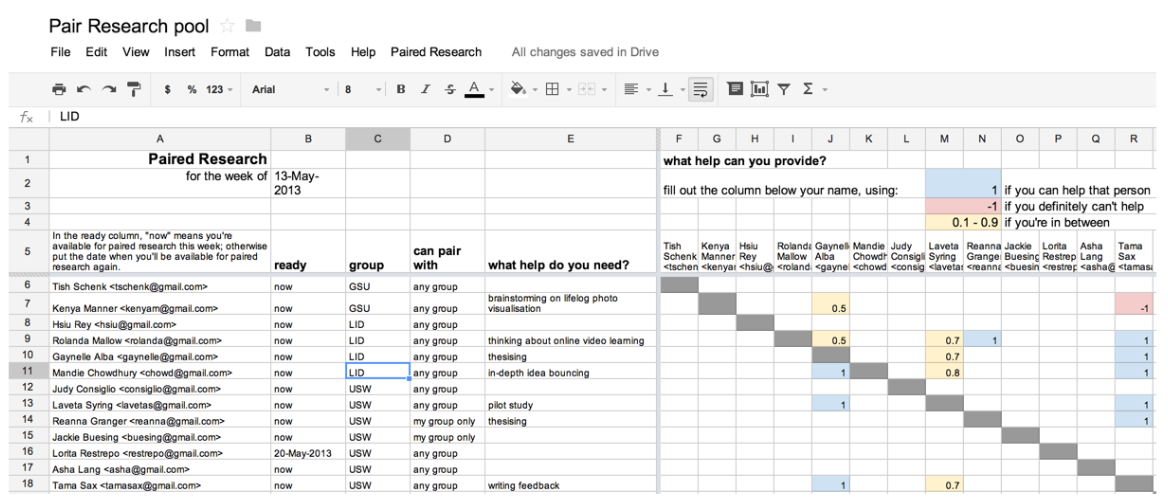
\includegraphics[scale=0.4]{figuras/pair_research.png}}\\
  \caption{Pair Research}{Hoja de excel utilizada para la matriz de preferencias y emparejamiento \protect\cite{miller_pair_2014}}
  \label{fig:pair_research}
\end{figure}
%\end{landscape}

La matriz de preferencias sirve para influir en la asignación de parejas de tal forma que aquellos con preferencia mutua positiva sean siempre emparejados mientras que aquellos con preferencia mutua negativa nunca sean emparejados y además se empareje de forma aleatoria a los miembros con preferencia mutua neutral. Para generar las vinculaciones, el sistema utiliza las preferencias ingresadas para formar un grafo ponderado cuyos nodos representan a los miembros del grupo y el grafo contiene un arco entre dos nodos si y solamente si ambos miembros tienen preferencias no negativas. El peso de una arista entre dos miembros es el promedio de sus preferencias mutuas más un plus siempre que ambos miembros no hayan sido emparejados recientemente. Por otro lado, para el caso de aquellos miembros con preferencias neutrales, el sistema agrega una perturbación aleatoria para hacer la asignación entre dichos miembros del grupo \cite{miller_pair_2014}.\\

La finalidad de la investigación en parejas o investigación en pares fue mejorar la productividad, el aprendizaje informal y la colaboración. En cuanto a la productividad, los resultados del estudio mostraron que los miembros se sintieron más motivados al trabajar usando esta técnica y realizaron satisfactoriamente sus trabajos asignados. Respecto al aprendizaje, se observó mejoras sobre herramientas específicas, habilidades, trabajos prácticos, aprendizaje sobre los demás miembros de grupo. Finalmente, en cuanto a colaboración, los integrantes de los grupos lograron interactuar con más personas de lo que usualmente lo harían lo cual incrementó sus oportunidades para colaboraciones futuras \cite{miller_pair_2014}.\\

\newpage
\subsection{Análisis comparativo}
En el siguiente cuadro ser resumen las características principales que nos ofrece cada una de las dos técnicas de aprendizaje colaborativo que han sido presentadas en los apartados anteriores.\\
\begin{longtable}{|L{8cm}|C{2.5cm}|C{2.5cm}|}
\caption{Técnicas de aprendizaje colaborativo}
\label{tab:tecnicasAC}\\
  \toprule[0.8mm]
  % after \\: \hline or \cline{col1-col2} \cline{col3-col4} ...
  CARACTERÍSTICAS & JIGSAW & PAIR RESEARCH \\
  \midrule[0.6mm]
  $\diamond$ Se aprende del compañero & \cmark & \cmark\\
  $\diamond$ Permite las revisiones de trabajo constantes & \xmark & \cmark\\
  $\diamond$ Desarrolla la creatividad & \cmark & \cmark\\
  $\diamond$ Mejora la comunicación del estudiante & \cmark & \cmark\\
  %$\diamond$ Favorece la integración del grupo	& \cmark & \xmark\\
  $\diamond$ Favorece el aprendizaje del tema a tratar & \cmark & \cmark\\
  $\diamond$ Existe un método para generar los emparejamientos & \xmark & \cmark\\
  $\diamond$ Se requiere la dirección de un profesor &	\cmark & \xmark	\\
  $\diamond$ Permite evitar conflictos interpersonales & \xmark &	\cmark\\
 % $\diamond$ Favorece al trabajo con personas conocidas & \cmark & \cmark\\
  $\diamond$ Favorece la integración con nuevas personas &	\cmark & \xmark \\	
  $\diamond$ El alumno elige con quién trabajar & \xmark & \cmark\\		
  $\diamond$ Los grupos se forman según estilos de aprendizaje & \xmark & \xmark\\		
  \bottomrule[0.8mm]
\end{longtable}

\newpage
\section{Frameworks para aplicaciones web}

\subsection{GoogleDrive Realtime API}

La API de GoogleDrive en tiempo real ofrece el trabajo colaborativo como un servicio para los archivos en Google Drive a través del uso de las transformaciones operativas. El API es una biblioteca JavaScript que ofrece a los desarrolladores objetos de colaboración, eventos y métodos para la creación de aplicaciones en las cuales se puedan realizar tareas colaborativas.\\

Esta API permite a los desarrolladores diseñar un modelo de datos común que se ve como un modelo local en memoria. Se pueden escribir código para manipular listas, arrays, matrices, maps, y objetos javascript propios del desarrollador. Cada vez que se modifique un modelo de datos, éste automáticamente cambiará para todos los usuarios presentes en el documento.\\

La API está basada en la misma tecnología de colaboración usada por GoogleDocs y por ello, cada vez que un modelo de datos es modificado, el cambio es aplicado inmediatamante a la copia local del documento y luego, la API envía una representación del cambio al servidor de tal forma que el cambio es guardado en el documento y comunicado a los demás colaboradores.\\

La API en tiempo real se encarga de todos los aspectos de la transmisión de datos, el almacenamiento y la resolución de conflictos cuando varios usuarios están editando un archivo. En general, la API nos brinda lo siguiente:

\begin{enumerate}
  \item Funciones para cargar y trabajar documentos en tiempo real.
  \item Objetos construídos colaborativamente(cadenas, listas, y mapas).
  \item La capacidad de crear objetos propios que puedan personalizarse.
  \item Eventos para la detección de cambios en el modelo de colaboración y detección del ingreso o salida de colaboradores.
\end{enumerate}
La API en tiempo real de GoogleDrive proporciona todas las herramientas que se necesitan para crear una aplicación colaborativa que no necesita correr en nuestro propio servidor.


%\subsection{Socket.IO}
%
%Socket.IO permite la comunicación basada en eventos bidireccional en tiempo real.
%Funciona en todas las plataformas, el navegador o dispositivo, centrándose también en la fiabilidad y la velocidad.
%\begin{itemize}
%  \item Análisis en tiempo real
%  \item Transmisión binaria. A partir de 1.0, es posible enviar cualquier tipo de archivo: imagen, audio, video.
%  \item Mensajería instantánea y chat
%  \item Colaboración de documentos. Permitir a los usuarios editar simultáneamente un documento y ver los cambios del otro.
%\end{itemize}

\subsection{Ideone API - Sphere Engine}
Sphere Engine, antes conocida como Ideone API, permite a los usuarios ejecutar código en múltiples lenguajes de manera online. Ideone es un compilador y una herramienta de depuración que soporta más de 60 lenguajes de programación. Através de la API, los desarrolladores pueden crear sus propias aplicaciones con fines educativos, personales o de negocios. Sphere Engine es un servicio web el cual puede ser accedido a través de protocolo SOAP.\\

Esta API posee las siguientes funcionalidades:

\begin{enumerate}
  \item Permite subir código fuente y compartirlo con otros usuarios.
  \item Permite ejecutar el código fuente con una data inicial en el lado servidor y en más de 60 lenguajes de programación diferentes.
  \item Permite descargar los resultados obtenidos en la ejecución del código fuente(salida, errores, información de compilación, tiempo de ejecución, uso de memoria, etc).
\end{enumerate}
\begin{figure}[h]
  \centering
  % Requires \usepackage{graphicx}
  \fbox{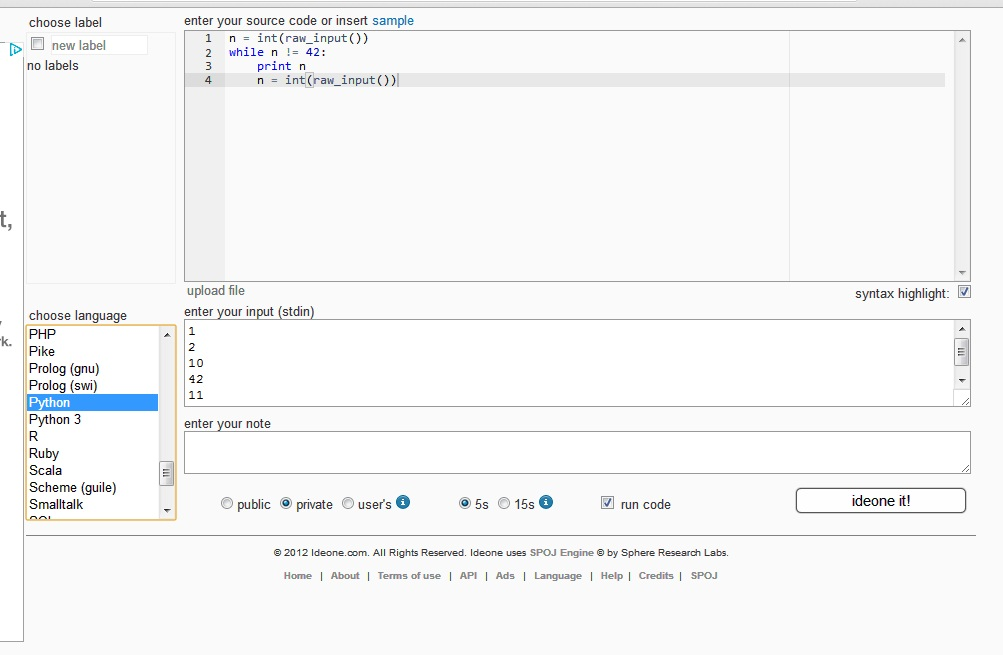
\includegraphics[scale=0.5]{figuras/ideone.jpg}}\\
  \caption[Ideone]{Interfaz gráfica de Ideone \protect\cite{ideone}}\label{fig:ideone}
\end{figure}

\newpage
\subsection{Análisis comparativo}
Tanto la API de GoogleDrive como la API de Ideone ofrecen características importantes para la elaboración de aplicaciones web de tiempo real, las mismas que se detallan en el siguiente cuadro comparativo.\\
\begin{longtable}{|L{10cm}|C{2cm}|C{2cm}|}
\caption{Frameworks para aplicaciones web.}
\label{tab:frameworks}\\
\toprule[0.8mm]
CARACTERÍSTICAS & Google Drive Realtime API	& Ideone API - Sphere Engine\\	
\midrule[0.6mm]
$\diamond$ Se implementa a través de Javascript	&\cmark	&\xmark	\\
$\diamond$ Creación y edición de listas, arrays, matrices, maps, objetos javascript personalizados		&\cmark	&\xmark	\\
$\diamond$ Detección de cambios	&\cmark	&\xmark	\\
$\diamond$ Detección de ingreso o salida de colaboradores	&\cmark	&\xmark	\\
$\diamond$ Ejecutar código en múltiples lenguajes de manera online	&\xmark	&\cmark	\\
$\diamond$ Servicio web vía protocolo SOAP	&\xmark	&\cmark	\\
$\diamond$ Permite cargar código fuente	&\xmark	&\cmark	\\
$\diamond$ Permite ejecutar código fuente	&\xmark	&\cmark	\\
$\diamond$ Permite subir data de prueba inicial	&\xmark	&\cmark	\\
$\diamond$ Permite descargar los resultados obtenidos en la ejecución	&\xmark	&\cmark	\\
\bottomrule[0.8mm]
\end{longtable}
\clearpage
\section{Análisis del estado del arte}
En este capítulo se presentaron algunas herramientas que sirven para el aprendizaje colaborativo. No obstante, para objetivos de esta tesis, se requiere un sistema que permita crear sesiones de clase jigsaw y tomar examenes, pero que estas clases y examenes sean sobre temas de algoritmos y programación siendo necesario entonces que el sistema permita al alumno desarrollar y compilar código fuente de forma colaborativa: características que los sistemas descritos en la \autoref{tab:herramientasAC} no las poseen de manera completa e integrada.\\

El sistema que se pretende desarrollar estará basado en el proceso para la elaboración de sesiones de clase usando la técnica de Jigsaw en la cual, tanto los grupos expertos y grupos jigsaw serán generados aleatoriamente por el sistema, garantizando así una mayor interacción entre los estudiantes, especialmente entre aquellos que se conocen por primera vez. \autoref{tab:tecnicasAC}.\\

El sistema a desarrollar también tendrá la particularidad de que permitirá a los estudiantes trabajar de forma colaborativa en la elaboración de archivos de código fuente, los cuales serán producto de las respuestas que dichos estudiantes darán a los problemas que les plantee el profesor durante la sesión de clase jigsaw. Por ende, para lograr este objetivo y tener dicha funcionalidad en el sistema, se usará la API de Ideone cuyas características se presentaron en la \autoref{tab:frameworks}.\\


\chapter{Aporte práctico}
\label{cap:aporte_practico}
En este capítulo se expone el desarrollo del Sistema Jigsaw Coding, el cual será realizado usando las mejores prácticas de RUP. También se describirá el uso de este sistema y se definirán las métricas  que permitirán medir la calidad del software implementado.

\section{Metodología de desarrollo}
Como ya se mencionó anteriormente, el Sistema Jigsaw Coding será elaborado usando las mejores prácticas de RUP, el mismo que a continuación se describe brevemente:\\

EL Proceso Unificado Rational(RUP) es un proceso de ingeniería de software que provee un enfoque para la asignación de tareas y responsabilidades durante el desarrollo de un software. Este tiene como objetivo asegurar la producción de un producto software de alta calidad que satisfaga los requerimientos de los usuarios finales dentro de un tiempo y presupuesto establecido \cite{rup_ibm_2014}. RUP, divide el proceso de desarrollo en fases y agrupa las diversas tareas y actividades en disciplinas, permitiendo organizar eficientemente cada uno de los artefactos que serán producto del desarrollo del sistema. \autoref{fig:rup}\\

\begin{figure}
  \centering
  % Requires \usepackage{graphicx}

  \caption[RUP]{Proceso de desarrollo de software - RUP.}
    \fbox{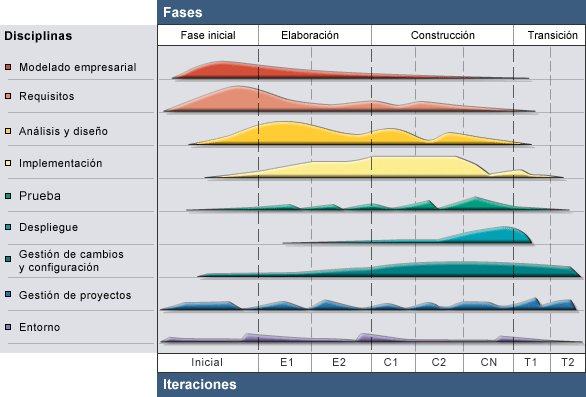
\includegraphics[scale=0.4]{figuras/rup.jpg}}\\
        \source{ \citeNP { rup_small }  }
  \label{fig:rup}
\end{figure}

Así mismo, RUP también es una guía para usar de manera efectiva el Lenguaje Unificado de Modelado (UML) que no es más que un lenguaje estándar que permite comunicar claramente los requerimientos, arquitecturas y diseños \cite{rup_ibm_2014}.\\

Para el desarrollo del Sistema Jigsaw Coding, se establecerán iteraciones semanales en las cuales se irá desarrollando cada una de las fases en las que RUP divide el ciclo de desarrollo de software: Inicio, Elaboración, Construcción y Transición. Los artefactos que serán entregados durante el proceso de desarrollo del sistema propuesto en esta tesis se mencionan en la  \autoref{tab:artefactos_rup}. Además, dichos artefactos se encuentran agrupados según la disciplina a la que pertenecen.

\begin{longtable}{|L{6cm}|L{7cm}|}
\caption{Artefactos del proceso de desarrollo del Sistema Jigsaw Coding}
\label{tab:artefactos_rup}\\
	\toprule[0.6mm]
    DISCIPLINA RUP & ARTEFACTO \\
    \midrule
    \multirow{2}{*}{Requisitos} & $\bullet$ Modelo de caso de uso\\
    \hhline{~~} & $\bullet$ Especificaciones de casos de uso\\
    \hhline{~~} & $\bullet$ Especificaciones suplementarias\\
    \midrule
    \multirow{5}{*}{Análisis y diseño} & $\bullet$ Diagrama de clases\\
    \hhline{~~} & $\bullet$ Modelo de datos\\
    %\hhline{~~} & $\bullet$ Prototipos de interfaz de usuario\\
    \hhline{~~} & $\bullet$ Documento de arquitectura de software\\
    \midrule
    \multirow{2}{*}{Implementación} & $\bullet$ Código fuente\\
    \hhline{~~} & $\bullet$ Sistema web desplegado\\
    %\midrule
    %\multirow{2}{*}{Prueba} & $\bullet$ Casos de prueba\\
    %\hhline{~~} & $\bullet$ Resultados de prueba\\
    \bottomrule[0.6mm]
\end{longtable}

%\clearpage
%Para el desarrollo del sistema web, se seguirá el siguiente cronograma, el mismo que se está orientado a seguir las actividades y tareas que plantea RUP. Se indica también las fechas en las cuales se estará aplicando el sistema al caso de estudio.
%
%\begin{figure}[!h]
%  \centering
%  % Requires \usepackage{graphicx}
%  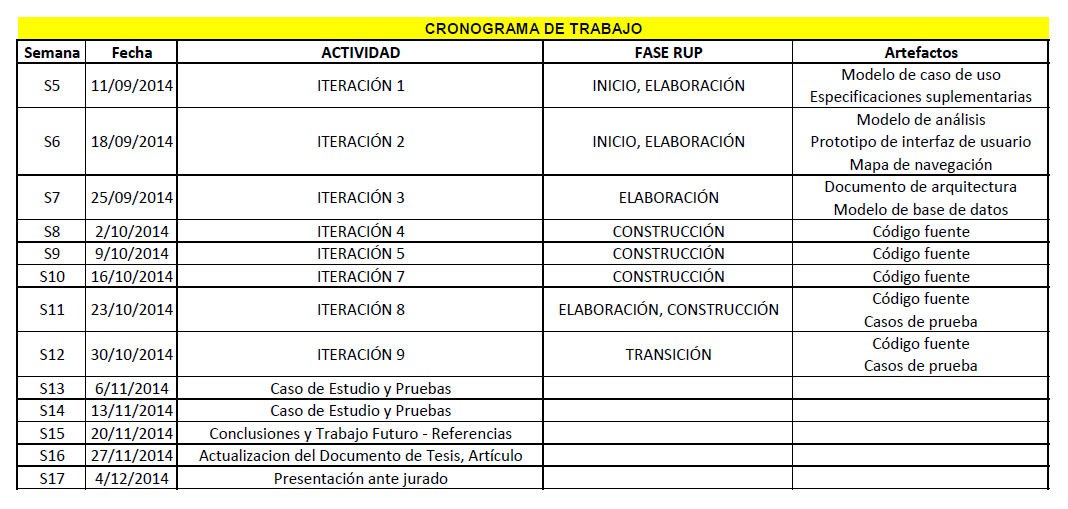
\includegraphics[scale=0.5]{figuras/cronograma}\\
%  \caption[CRONOGRAMA]{Cronograma de trabajo}\label{fig:cronograma}
%\end{figure}

%\begin{longtable}{|L{2.5cm}|L{2cm}|L{5cm}|L{5cm}|}
%\caption{CRONOGRAMA}
%\label{tab:cronograma}\\
%    \hline
%    ITERACIÓN & FECHA & FASE RUP & ARTEFACTO \\
%    \hline
%    1 &	11-09-2014	&	INICIO, ELABORACIÓN	& Modelo de caso de uso, Especificaciones suplementarias\\
%
%    \hline
%\end{longtable}
\clearpage
\section{Desarrollo del Sistema Jigsaw Coding}
En esta sección se presenta una descripción a alto nivel sobre los artefactos elaborados durante el proceso de desarrollo del sistema.

\subsection{Modelo de casos de uso}
El modelo de casos de uso permite mostrar de manera general las funcionalidades del sistema. Inicialmente, se indica el catálogo de actores que interactúan con el sistema y luego se presenta la descripción de lo casos de uso más resaltantes. La especificación de todos los casos de uso se encuentra en el \autoref{apendice.A}\\

Los casos de uso son una forma de especificación de requisitos funcionales. Un caso de uso es la descripción de una secuencia de interacciones entre el sistema y un o más actores.

\subsubsection{Catálogo de actores}
En el la \autoref{fig:cap4_actores} se puede ver los actores que participan en el Sistema Jigsaw Coding y en la \autoref{tab:cap4_actores} se encuentra una breve descripción de cada uno de ellos.
\begin{figure}[h]
	\centering
	% Requires \usepackage{graphicx}
	\fbox{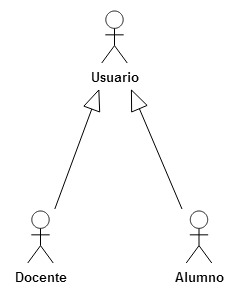
\includegraphics[scale=0.8]{figuras/casosdeuso/actores.jpg}}\\
	\caption[Diagrama de actores]{Diagrama de actores}
	\label{fig:cap4_actores}
\end{figure}
\clearpage
\begin{longtable}{L{3cm}L{7cm}}
	\caption{Actores}
	\label{tab:cap4_actores}\\
	\toprule[0.8mm]
	ACTOR & DESCRIPCIÓN \\
	\midrule[0.6mm]
	Usuario & Persona que usará el sistema web de tiempo real para el aprendizaje colaborativo.\\
	\midrule
	Docente & Es la persona responsable de crear y dirigir las sesiones de clase que serán aplicadas a los alumnos. Además, el docente es el responsable de las evaluaciones que rendirán los alumnos una vez terminada cada sesión de clase.\\
	\midrule
	Alumno & Es la persona que será instruida en temas de algoritmos y programación a través de cada sesión diseñada por el docente.\\
	\bottomrule[0.8mm]
\end{longtable}

\subsubsection{Casos de uso}
En la tabla siguiente se presenta la descripción breve de los casos de uso obtenidos para el Sistema Jigsaw Coding, estos son especificados de una manera más detallada en el \autoref{apendice.A}
\begin{longtable}{L{4cm}L{9cm}}
	\caption{Casos de uso}
	\label{tab:cap4_casosdeuso}\\
	\toprule[0.8mm]
	CASO DE USO & DESCRIPCIÓN \\
	\midrule[0.6mm]
	Registrar alumno & Este caso de uso define los pasos que el usuario con perfil docente debe seguir para poder registrar un alumno en el sistema.\\
	\midrule
	Crear Problema & El caso de uso crear problema detalla la interacción entre el sistema y el usuario docente cada vez que éste necesite crear un problema o ejercicio en el sistema.\\
	\midrule
	Crear sesión jigsaw & Este caso de uso describe la secuencia de pasos que se debe seguir para poder crear una sesión de clase basada en la técnica de aprendizaje colaborativo jigsaw.\\
	\midrule
	Asignar alumnos a sesión jigsaw & Las sesiones jigsaw necesitan tener alumnos y ese es el objetivo que tine este caso de uso.\\
	\midrule
	Generar grupos & Mediante este caso de uso, el Sistema Jigsaw Coding realiza la creación de grupos expertos y grupos jigsaw y a cada uno de ellos les asigna alumnos de forma aleatoria.\\
	\midrule
	Asignar problemas a grupos expertos & En este caso de uso se describe cómo el usuario docente puede asignar un problema a cada grupo experto generado por el sistema para una determinada sesión jigsaw.\\
	\midrule
	Crear examen & El caso de uso detalla la manera en la que el usuario docente puede crear un examen, el mismo que será usado para la fase de evaluación de la sesión jigsaw.\\
	\midrule
	Definir horario de reunión de expertos & Este caso de uso sirve para establecer la fecha y hora de inicio de la reunión de expertos así como su respectiva duración.\\
	\midrule
	Definir horario de reunión jigsaw & Este caso de uso sirve para establecer la fecha y hora de inicio de la reunión jigsaw así como su respectiva duración.\\
	\midrule
	Definir horario de examen & Este caso de uso sirve para establecer el intervalo de tiempo en el cual se puede acceder a examen así como también su respectiva duración.\\
	\midrule
	Unirse a reunión de expertos & Este caso de uso le sirve al usuario alumno para poder ingresar a la reunión de expertos y desarrollar el problema asignado junto con los demás integrantes del grupo.\\
	\midrule
	Unirse a reunión jigsaw & Este caso de uso le sirve al usuario alumno para poder ingresar a la reunión jigsaw y desarrollar los respectivos problemas junto con los demás integrantes del grupo. \\
	\midrule
	Resolver problema & El caso de uso describe la interacción entre el usuario alumno y el sistema cada vez que se requiere resolver un problema asignado por el usuario docente.\\
	\midrule
	Rendir examen & El caso de uso le permite al usuario alumno acceder al examen y visualizar cada una de las preguntas que debe resolver.\\
	\midrule
	Consultar al grupo & Este caso de uso describe la manera en la que un usuario alumno puede consultar con los demás integrantes de su grupo experto o grupo jigsaw.\\
	\bottomrule[0.8mm]
\end{longtable}

El Sistema Jigsaw Coding tiene como característica principal el permitir a los usuarios de perfil alumno poder resolver problemas de programación que el docente asigne para la sesión jigsaw. Este requisito está descrito en el caso de uso \textbf{Resolver problema} que se presenta en la \autoref{fig:c4_cus_resolver_problema}. 

\begin{figure}
	\centering	
	\fbox{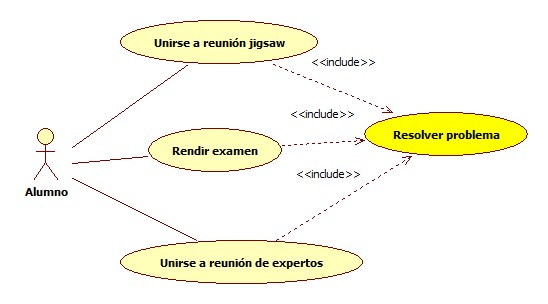
\includegraphics[scale=0.4]{figuras/casosdeuso/resolver_problema}}
	\caption{Caso de uso Resolver problema}
	\label{fig:c4_cus_resolver_problema}
\end{figure}

Como se observa en la \autoref{fig:c4_cus_resolver_problema}, el caso de uso Resolver problema se encuentra como parte de los casos de uso Unirse a reunión de expertos, Unirse a reunión jigsaw y Rendir examen, y esto es porque, en cada una de las fases de la sesión jigsaw que se elabora en el sistema, se asignan problemas de algoritmos y programación que los alumnos deben desarrollar ya sea de manera grupal, o individual cuando se trata de un examen. El desarrollo de estos problemas se realiza en un editor de código fuente y luego se compila para obtener los resultados de la solución elaborada. En la tabla \autoref{tab:c4_cus_resolver_problema} se muestra la descripción del caso de uso resolver problema así como también su correspondiente flujo básico. Para más detalle ver \autoref{apendice.A}.
%\clearpage

\begin{longtable}{|c|L{10cm}|}
	\caption{Caso de uso resolver problema.}
	\label{tab:c4_cus_resolver_problema}\\
	\toprule[0.5mm]
	% after \\: \midrule or \cline{col1-col2} \cline{col3-col4} ...
	Descripción & El caso de uso inicia cuando el alumno ingresa a una reunión o a un examen en el cual debe desarrollar un problema asignado por el docente. \\  \midrule
	Flujo básico & \begin{enumerate}
		\item El alumno escribe la solución al problema en el editor de código fuente.
		\item El alumno ingresa los datos de prueba en el panel correspondiente.
		\item El alumno selecciona la opción Compilar para compilar su código fuente. 
		\item El sistema compila y ejecuta el código del alumno.
		\item El sistema muestra los resultados de la ejecución.
	\end{enumerate}\\
	\bottomrule[0.5mm]
\end{longtable}

\subsection{Arquitectura del Sistema}
En esta sección se provee una vista general de la arquitectura para el Sistema Jigsaw Coding, la misma que permite tener una visión sobre la estructura del sistema, funcionalidades y demás aspectos técnicos que el sistema requiere. Para un mayor detalle de la arquitectura, revisar el \autoref{apendice.C}.\\

La meta principal del Sistema Jigsaw Coding es que opere sobre una plataforma web y para esto es necesario utilizar herramientas y tecnologías que permitan desarrollar sistemas web. Además debe tenerse en cuenta ciertos frameworks que ayuden en la elaboración de la parte colaborativa del sistema.
\clearpage
\subsubsection{PlayFramework 2.2.4}
Play es framework open source de Java y Scala que integra componentes y APIs necesarios para el desarrollo moderno de aplicaciones web. Play sigue el patrón de arquitectura Modelo - Vista - Controlador y uno de sus objetivos es optimizar la productividad del desarrollador a través del uso de configuraciones estandarizadas, recompilación automática del código fuente y la visualización de errores directamente en el navegador.

%\subsubsection{Persistencia}
%La persistencia se logrará utilizando una base de datos relacional y el mapeo de entidades a tablas estará a cargo del ORM Ebean que por defecto viene incluído en el framework Play.
%
%\subsubsection{Seguridad}
%La seguridad del sistema está basada en perfiles. La aplicación contendrá los siguientes puntos:
%
%\begin{itemize}
%	\item Autenticación: Cada usuario deberá identificarse con su email y password para poder acceder al sistema.
%	\item Autorización: El sistema cuenta con dos perfiles(Docente y Alumno) y dependiendo de ello, el usuario podrá ingresar a diferentes partes del sistema.
%	\end{itemize}

\subsubsection{Vista lógica}
\begin{figure}
\centering
% Requires \usepackage{graphicx}
\fbox{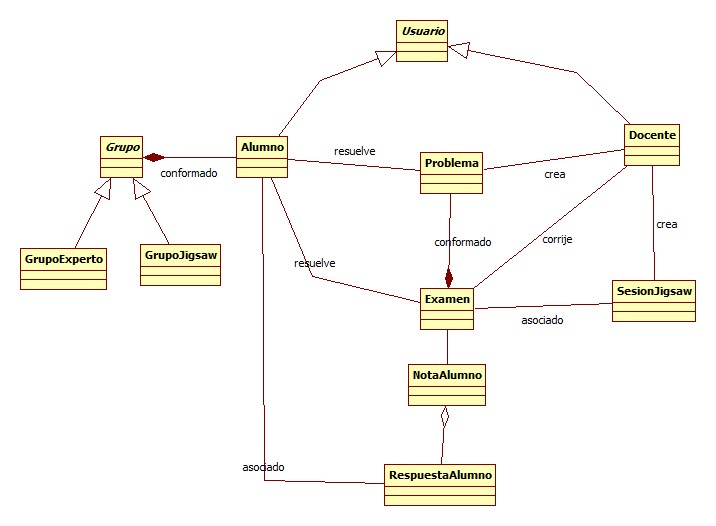
\includegraphics[scale=0.5]{figuras/sad/diagrama_de_clases.jpg}}\\
\caption{Diagrama de Clases}\label{fig:c4_diagrama_de_clases}
\end{figure}

Tal como se muetra en el diagrama de clases de la \autoref{fig:c4_diagrama_de_clases}, el Sistema Jigsaw Coding permite el acceso a Usuario lo cuales pueden ser de dos tipos: Docente o Alumno. El docente puede crear problemas y además es el encargado de crear las sesiones jigsaw. El docente también es quien crea los examenes, los cuales están conformados por un conjunto de problemas y cada examen es resuelto por los alumnos, quienes para tal objetivo, deben resolver los problemas que componen cada examen. Por otro lado, los alumnos también resuelven problemas cada vez que se encuentran dentro de un grupo de expertos o un grupo jigsaw. Naturalmente, los examenes son evaluados por el docente y éste les asigna una nota a cada una de las respuestas que los alumnos envía al terminar su examen.

\subsubsection{Vista de Desarrollo}
La vista de desarrollo muestra el sistema desde la perspectiva del programador y se ocupa de la gestión del software a implementar. Esto es, en esta vista se describe cómo estará dividido el sistema Jigsaw Coding en paquetes y las dependencias que hay entre ellos. Ver \autoref{fig:c4_diagrama_de_paquetes}.
\begin{figure}[!h]
	\centering
	% Requires \usepackage{graphicx}
	\fbox{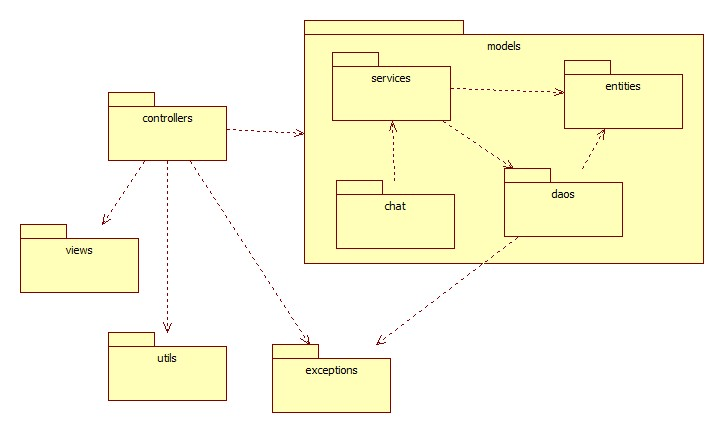
\includegraphics[scale=0.5]{figuras/sad/diagrama_de_paquetes.jpg}}\\
	\caption{Diagrama de Paquetes}\label{fig:c4_diagrama_de_paquetes}
\end{figure}
\begin{itemize}
	\item \textbf{controllers}\\Este paquete contiene todas las clases Controladores que sirven para gestionar el ruteo de páginas del sistema.
	\item \textbf{models}\\En este paquete se encuentran las clases de Servicios, Entidades y Acceso a Datos que son requeridas para el sistema.
	\item \textbf{views}\\Este paquete contiene todas las plantillas (\emph{*.scala.html}) que permitirán renderizar las páginas web del sistema.
\end{itemize}

\section{Uso del Sistema Jigsaw Coding} 
El Sistema Jigsaw Coding es un aplicativo web que permite crear sesiones de clase basadas en la técnica de aprendizaje colaborativo de rompecabezas o también llamada técnica jigsaw. Estas sesiones de clase están orientadas a la resolución de ejercicios y problemas relacionados con temas de algorítmica y programación en lenguajes Java, C++ y Python.\\

El sistema posee dos perfiles de usuario: Docente y Alumno. El primero permite al usuario crear ejercicios y problemas de algoritmos y programación. Dentro del perfil docente, el usuario tiene la capacidad para crear a los usuarios alumnos que participarán en la sesión de clase jigsaw para luego asignarlos a las sesiones jigsaw para que el sistema genere los grupos expertos y grupos jigsaw. Posteriormente a ello, el usuario con perfil docente podrá asignar a cada grupo experto un problema o ejercicio a resolver, y luego asignar la fecha y duración para cada fase de la dinámica jigsaw (Reunión de Expertos, Reunión Jigsaw y Evaluación). Para la fase de evaluación, el sistema permite al usuario crear diversos examenes con problemas y ejercicios a los cuales se les asigna un puntaje; luego, cada examen se asigna a una determinada sesión jigsaw. Finalmente, el usuario docente podrá calificar la solución que cada uno de los participantes de la sesión jigsaw elabore para un determinado examen.\\

En el perfil Alumno, el usuario puede participar de las reuniones de expertos y reunions jigsaw, en las cuales se deberá resolver los problemas asignados a cada grupo experto o jigsaw. Esta soluciones serán construidas de forma colaborativa entre todos los miembros de cada grupo. El sistema brinda al usuario un chat para poder comunicarse con los demás integrantes de su grupo experto o jigsaw. Es importante resaltar también, que durante la resolución de cada problema el usuario puede ir ejecutando el código fuente y ver los resultados de dicha ejecución. Cuando el usuario se encuentre en la fase de evaluación, éste podrá resolver su examen de forma individual y dentro del tiempo establecido por el docente.\\

\subsection{Login} 
Para acceder al Sistema Jigsaw Coding, el usuario debe estar su \textbf{email} y su \textbf{password} en el formulario que se muestra en la \autoref{fig:sjc_login}.\\

\begin{figure}
	\centering
	\caption[SJC Login]{Sistema Jigsaw Coding - Login}
	\label{fig:sjc_login}
	\fbox{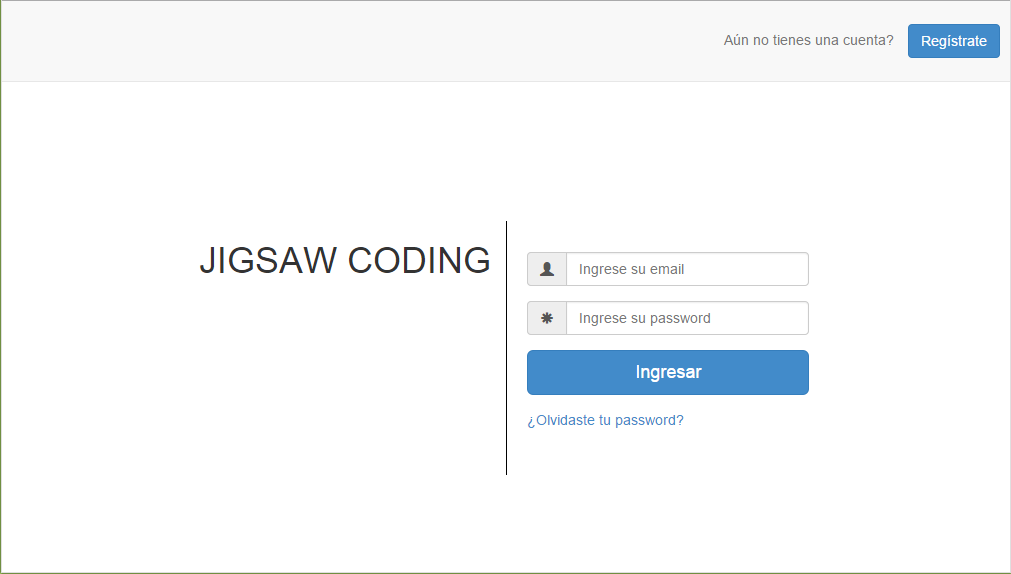
\includegraphics[scale=0.3]{figuras/usodelsistema/login}}	
\end{figure}

Si el usuario no está registrado en el sistema, debe ingresar a la opción \textbf{Regístrate} y completar los datos solicitados por el sistema. \autoref{fig:login_registrate}. Luego de este paso, el usuario tendrá acceso al sistema a través de un perfil Docente.\\

\begin{figure}
	\centering
	\caption[SJC Registrate]{Sistema Jigsaw Coding - Regístrate}
	\label{fig:login_registrate}
	\fbox{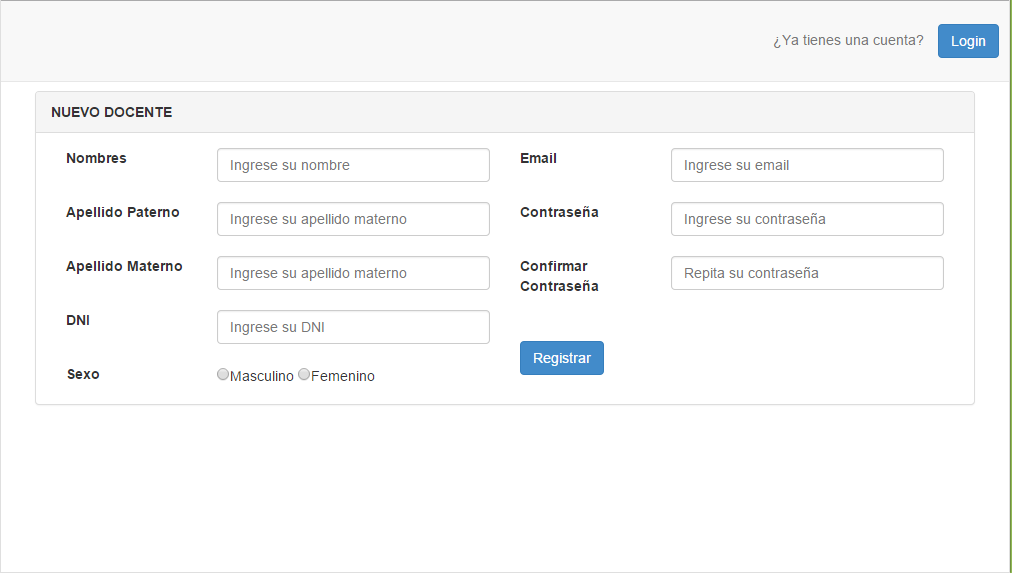
\includegraphics[scale=0.4]{figuras/usodelsistema/login_registrate}}	
\end{figure}

Si el acceso al sistema se dió exitosamente, entonces el usuario podrá visualizar la página de inicio con todas las opciones permitidas para el perfil docente. \autoref{fig:inicio}.

\begin{figure}
\centering
\caption[SJC Inicio]{Sistema Jigsaw Coding - Bienvenido}
\label{fig:inicio}
\fbox{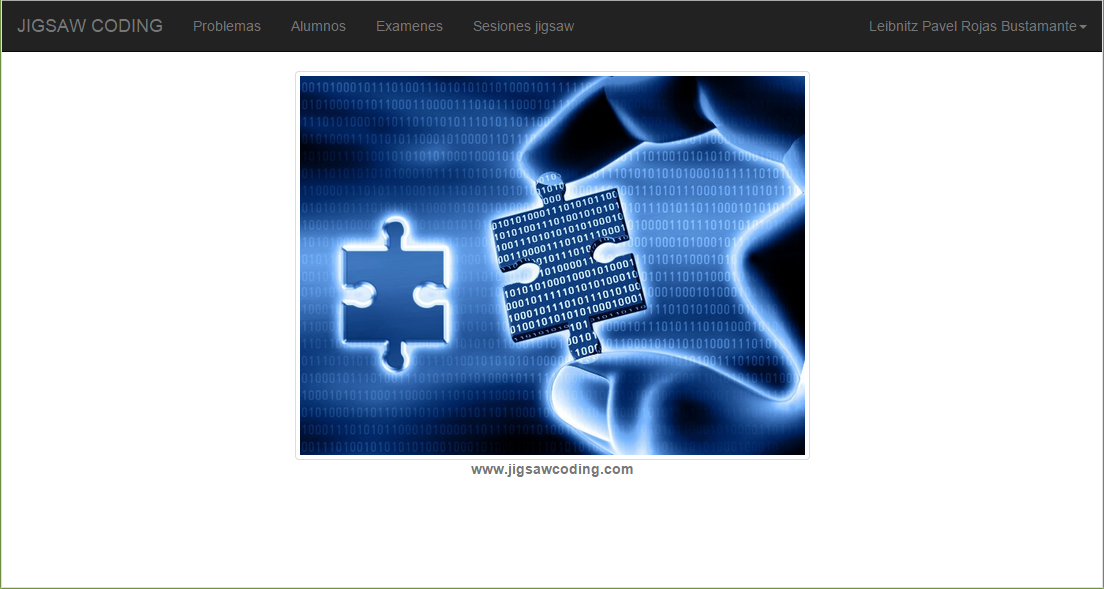
\includegraphics[scale=0.4]{figuras/usodelsistema/docente/inicio}}
\end{figure}
%\clearpage

\subsection{Problemas}
Al acceder al módulo problemas, el usuario visualizará el listado de problemas que ha creado hasta el momento y en dicho listado, se mostrará el título y enunciado de cada problema. Además se podrá filtrar los problemas según el título o enunciado. \autoref{fig:problemas_inicio}.

\begin{figure}
\centering
\caption[SJC Problemas]{Sistema Jigsaw Coding - Inicio del módulo Problemas}
\label{fig:problemas_inicio}
\fbox{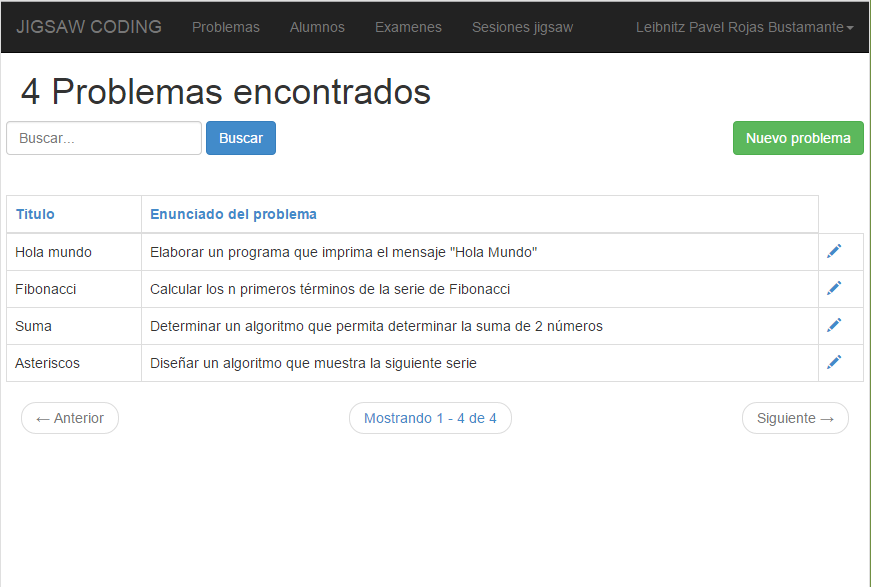
\includegraphics[scale=0.4]{figuras/usodelsistema/docente/problemas_inicio}}
\end{figure}

\subsubsection{Crear problema}

Para crear un nuevo problema se debe acceder a menú Problemas y luego presionar el botón \textbf{Nuevo problema}. \autoref{fig:problemas_nuevo}. Luego, se debe ingresar el título y enunciado del problema y presionar el botón \textbf{Guardar}.

\begin{figure}
\centering
\caption[SJC Nuevo problema]{Sistema Jigsaw Coding - Nuevo problema}
\label{fig:problemas_nuevo}
\fbox{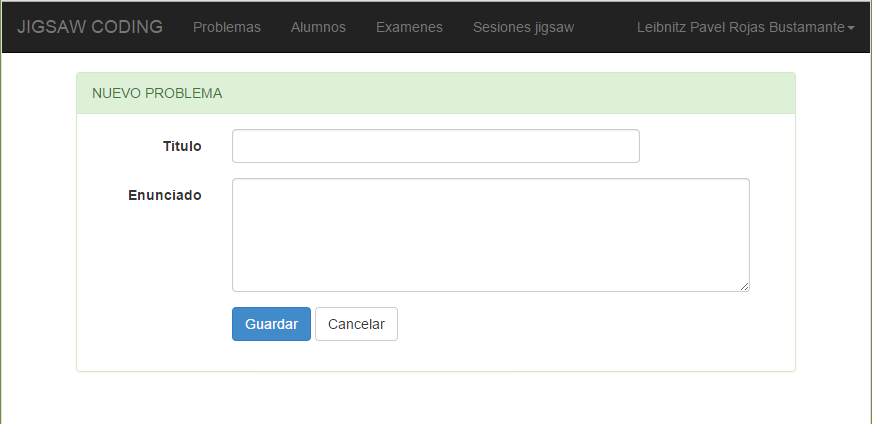
\includegraphics[scale=0.5]{figuras/usodelsistema/docente/problemas_nuevo}}
\end{figure}

\subsubsection{Editar problema}
En la página principal del módulo Problemas se puede ver cada problema creado y para cada uno, existe un botón que permite editar dicho problema. Con esta opción se puede modificar el título o enunciado del problema y también se puede eliminar dicho problema del sistema. Ver figura \autoref{fig:problemas_editar}.

\begin{figure}
\centering
\caption[SJC Editar problema]{Sistema Jigsaw Coding - Editar problema}
\label{fig:problemas_editar}
\fbox{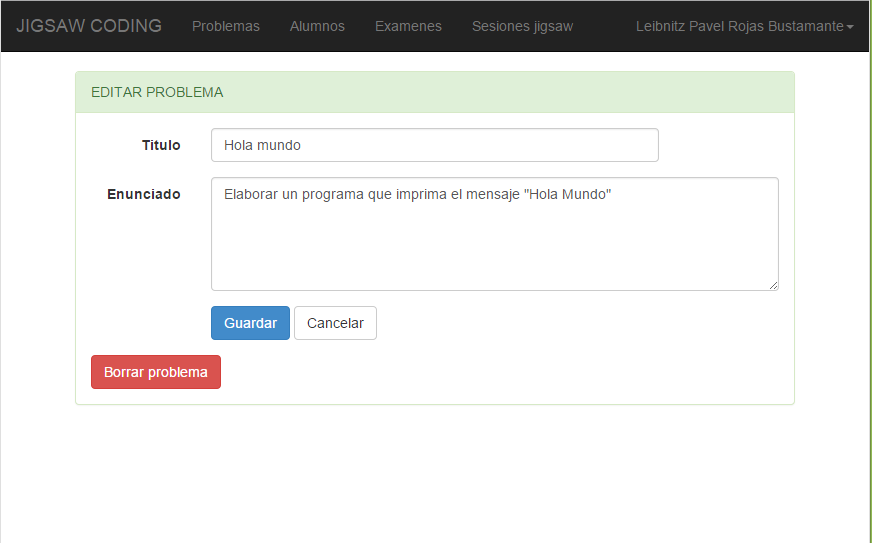
\includegraphics[scale=0.5]{figuras/usodelsistema/docente/problemas_editar}}
\end{figure}

\subsection{Alumnos}
Tal como se puede apreciar en la \autoref{fig:alumnos_inicio}, al acceder al módulo alumnos, el usuario visualizará el listado de alumnos registrados hasta el momento y en dicho listado, se mostrará los apellidos, nombres y dni de cada alumno. Además se podrá filtrar dichos alumnos con la opción Buscar.

\begin{figure}
	\centering
	\caption[SJC Alumnos]{Sistema Jigsaw Coding - Inicio del módulo Alumnos}
	\label{fig:alumnos_inicio}
	\fbox{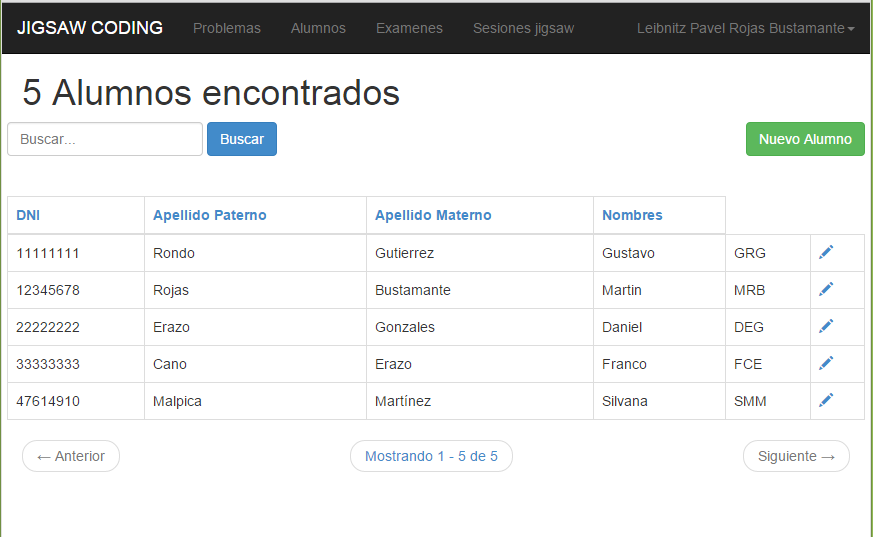
\includegraphics[scale=0.5]{figuras/usodelsistema/docente/alumnos_inicio}}
\end{figure}

\subsubsection{Registrar alumno}

Para registrar un nuevo alumno se debe acceder a menú Alumnos y luego presionar el botón \textbf{Nuevo Alumno}. \autoref{fig:alumnos_nuevo}. Luego, se debe completar los campos solicitados por el sistema y presionar el botón \textbf{Registrar}.

\begin{figure}
	\centering
	\caption[SJC Nuevo alumno]{Sistema Jigsaw Coding - Nuevo Alumno}
	\label{fig:alumnos_nuevo}
	\fbox{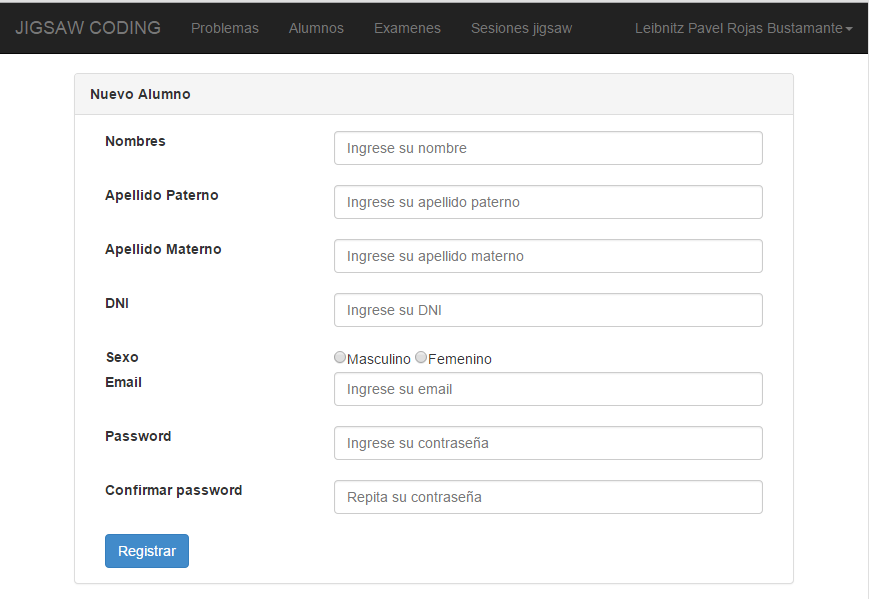
\includegraphics[scale=0.4]{figuras/usodelsistema/docente/alumnos_nuevo}}
\end{figure}

\subsection{Examenes}
Al acceder al módulo examenes, el usuario visualizará el listado de examenes registrados hasta el momento y en dicho listado, se mostrará el título del examen y los nombres de los problemas que forman parte del examen. Además se podrá filtrar dichos examenes con opción Buscar. \autoref{fig:examenes_inicio}.

\begin{figure}
	\centering
	\caption[SJC Examenes]{Sistema Jigsaw Coding - Inicio del módulo Examenes}
	\label{fig:examenes_inicio}
	\fbox{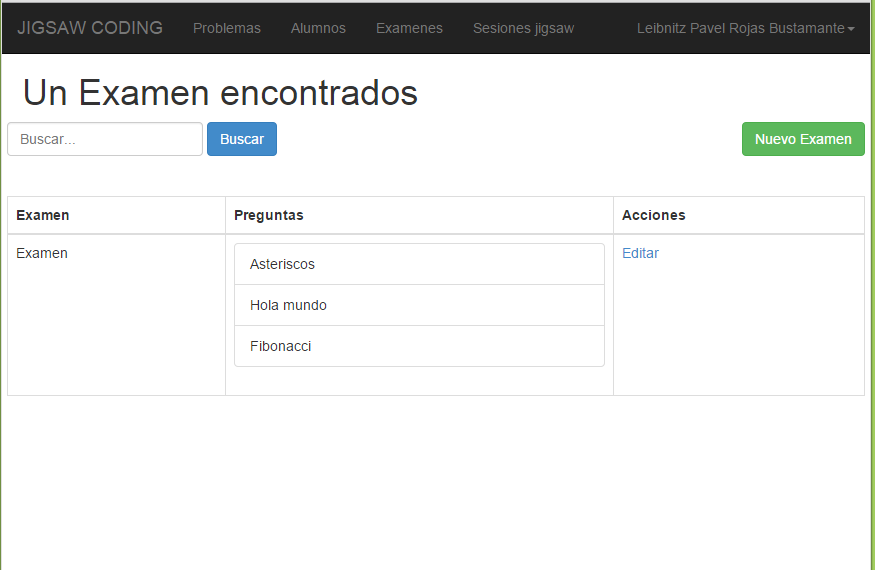
\includegraphics[scale=0.4]{figuras/usodelsistema/docente/examenes_inicio}}
\end{figure}
\subsubsection{Crear examen}

Para registrar un nuevo examen se debe acceder a menú Examenes y luego presionar el botón \textbf{Nuevo Examen} con lo cual el usuario podrá ver la interfaz para asignar los problemas al examen. \autoref{fig:examenes_nuevo}. \\

\begin{figure}
	\centering
	\caption[SJC Nuevo examen]{Sistema Jigsaw Coding - Nuevo Examen}
	\label{fig:examenes_nuevo}
	\fbox{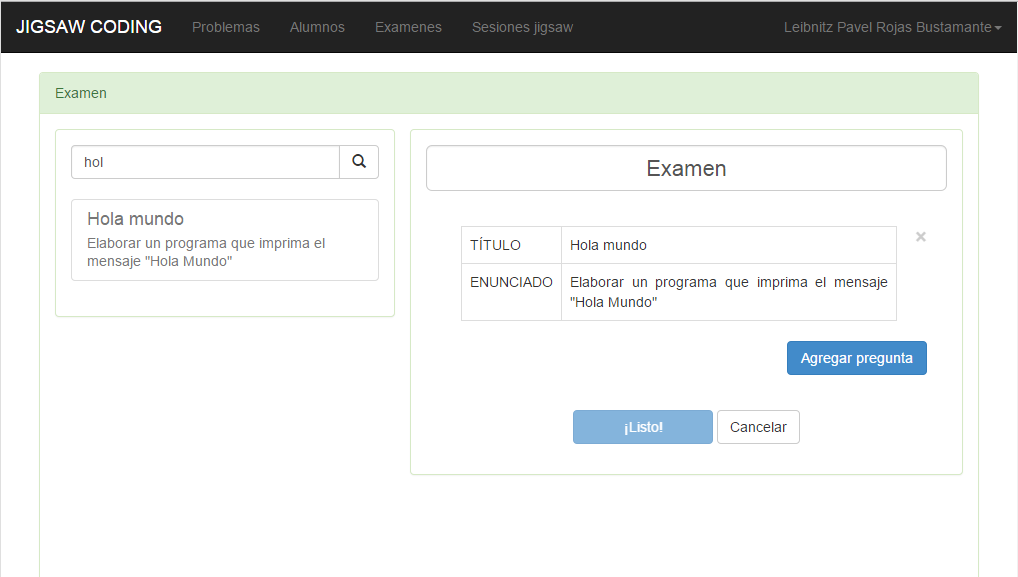
\includegraphics[scale=0.4]{figuras/usodelsistema/docente/examenes_nuevo}}
\end{figure}

La asignación de problemas al examen se realiza siguiendo los pasos descritos a continuación:

\begin{enumerate}
	\item En el campo \textbf{Buscar} escriba el nombre del problema que desea agregar.
	\item Haga click en el problema y automáticamente éste se mostrará en el panel del Examen.
	\item Presione el botón Agregar pregunta.
	\item Haga click en el problema para habilitar las opciones de asignar puntaje al problema y establezca la puntación para el problema. 
	\item Presione nuevamente el problema para guardar el puntaje.
	\item Agregue los problemas que sean necesarios hasta que el marcador de puntaje de examen sume un total de 20 puntos. Luego entonces presione el botón \textbf{Listo} para guardar el examen.
\end{enumerate}

\subsection{Sesiones Jigsaw}
Al acceder al módulo sesiones jigsaw, el usuario podrá ver el listado de sesiones jigsaw creadas hasta el momento y en dicho listado se encontrará la respectiva información sobre la reunión de expertos, reunión jigsaw y evaluación. \autoref{fig:sesionesjigsaw_inicio}.

\begin{figure}
\centering
\caption{Sistema Jigsaw Coding - Inicio del módulo sesiones jigsaw}
\label{fig:sesionesjigsaw_inicio}
\fbox{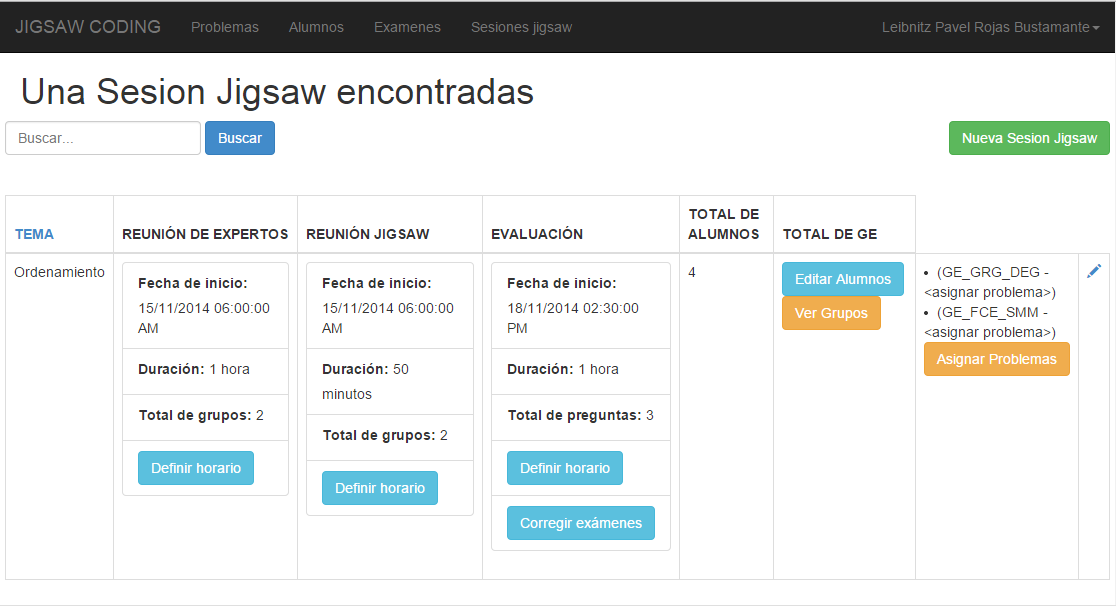
\includegraphics[scale=0.5]{figuras/usodelsistema/docente/sesionesjigsaw_inicio}}
\end{figure}
%\clearpage
\subsubsection{Crear sesión jigsaw}
A continuación se describen los pasos para crear una sesión jigsaw.
\begin{enumerate}
	\item Presione el botón \textbf{Nueva Sesión Jigsaw}.
	\item Indique el total de grupos expertos y el tema de la sesión jigsaw. \autoref{fig:sesionesjigsaw_nuevo_01}
	\begin{figure}
	\centering
	\caption[SJC Sesiones jigsaw]{Sistema Jigsaw Coding - Nueva sesión jigsaw}
	\label{fig:sesionesjigsaw_nuevo_01}
	\fbox{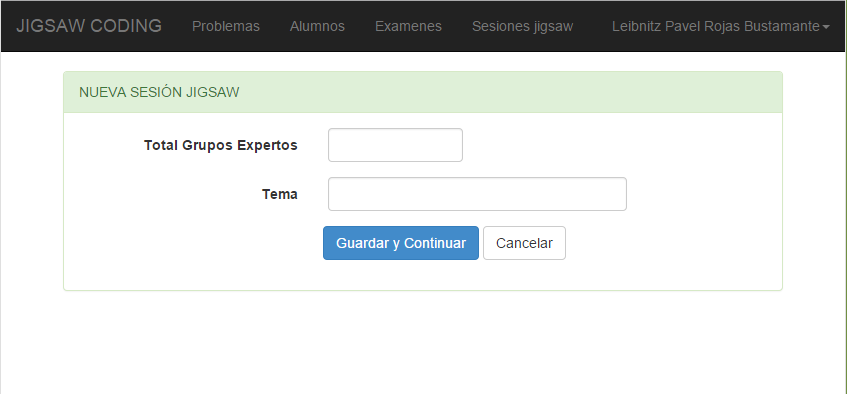
\includegraphics[scale=0.5]{figuras/usodelsistema/docente/sesionesjigsaw_nuevo_01}}
	\end{figure}
	\item En el listado de sesiones jigsaw aparecerá una nueva sesión.\autoref{fig:sesionesjigsaw_nuevo_02}
	\begin{figure}
	\centering
	\caption{Sistema Jigsaw Coding - Nueva sesión jigsaw}
	\label{fig:sesionesjigsaw_nuevo_02}
	\fbox{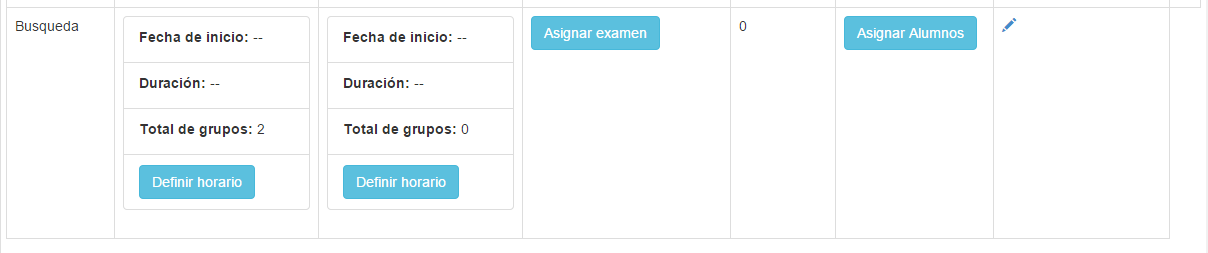
\includegraphics[scale=0.5]{figuras/usodelsistema/docente/sesionesjigsaw_nuevo_02}}
	\end{figure}
	\item Presione el botón agregar alumnos para definir qué alumnos formarán parte de la sesión jigsaw. Mueva los alumnos desde el panel de Alumnos Disponibles hacia el panel de la Sesión Jigsaw y presione el botón \textbf{Guardar}.  \autoref{fig:sesionesjigsaw_nuevo_03}
	\begin{figure}
	\centering
	\caption{Sistema Jigsaw Coding - Nueva sesión jigsaw}
	\label{fig:sesionesjigsaw_nuevo_03}
	\fbox{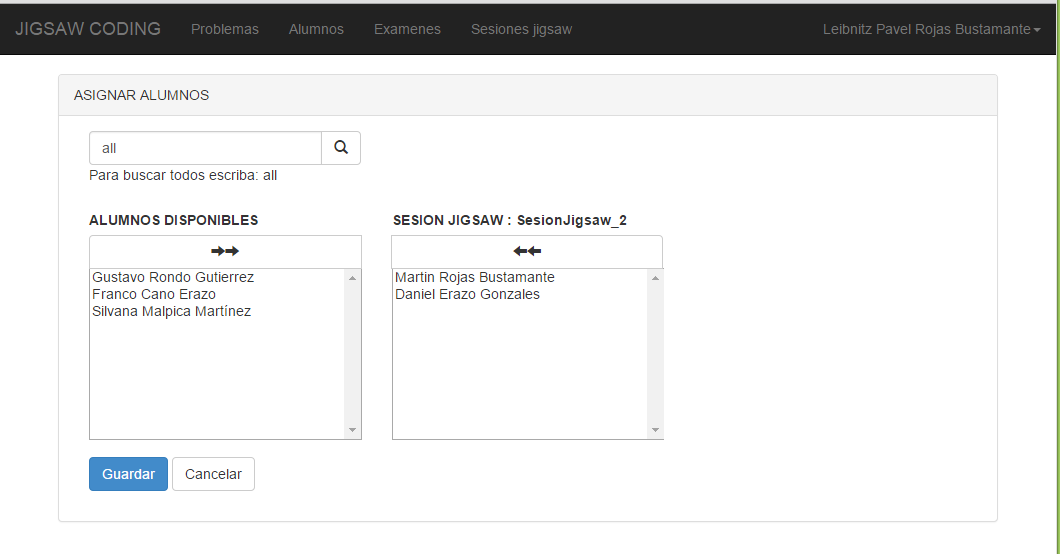
\includegraphics[scale=0.5]{figuras/usodelsistema/docente/sesionesjigsaw_nuevo_03}}
	\end{figure}
	\item Luego de agregar a los alumnos, se habilitará el botón \textbf{Generar Grupos} el cual deberá presionar para que el sistema genere de forma aleatoria los Grupos expertos y los grupos jigsaw. \autoref{fig:sesionesjigsaw_nuevo_04}
	\begin{figure}
		\centering
		\caption{Sistema Jigsaw Coding - Nueva sesión jigsaw}
		\label{fig:sesionesjigsaw_nuevo_04}
		\fbox{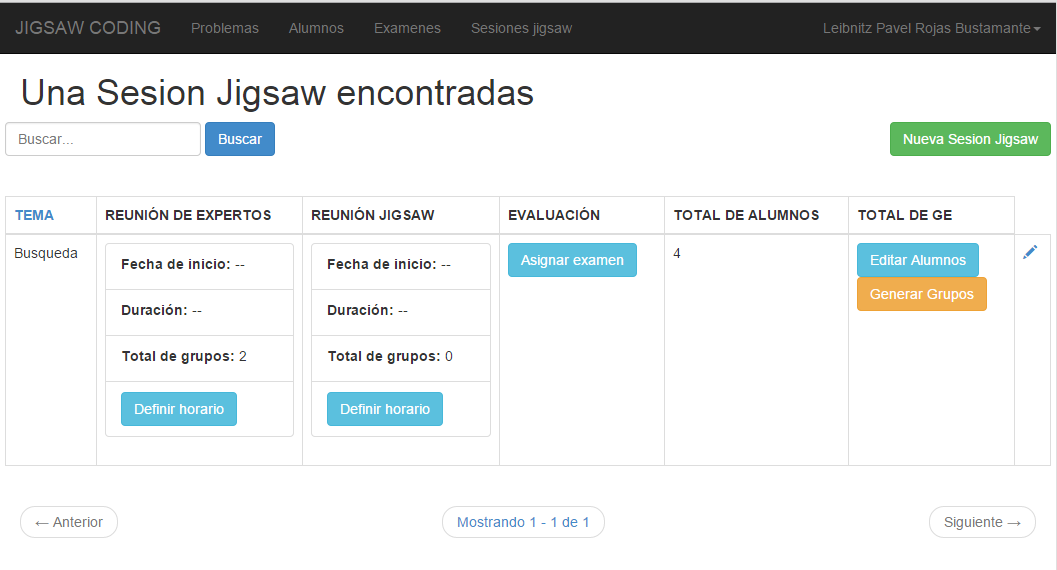
\includegraphics[scale=0.5]{figuras/usodelsistema/docente/sesionesjigsaw_nuevo_04}}
	\end{figure}
	\item Si la generación de grupos se realizó exitosamente, el sistema le mostrará los grupos sus respectivos integrantes. \autoref{fig:sesionesjigsaw_nuevo_05}
	\begin{figure}
		\centering
		\caption{Sistema Jigsaw Coding - Nueva sesión jigsaw}
		\label{fig:sesionesjigsaw_nuevo_05}
		\fbox{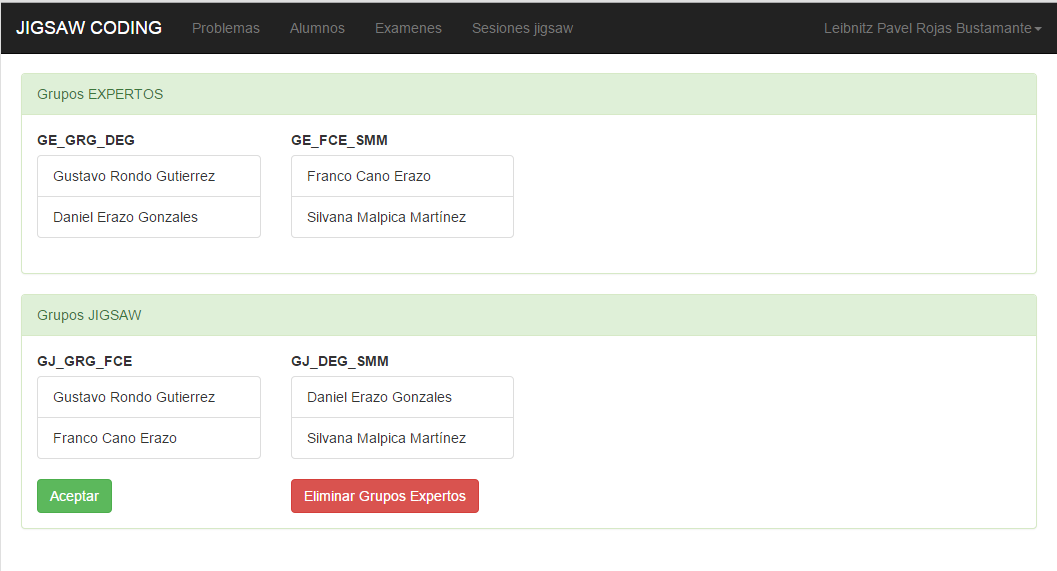
\includegraphics[scale=0.5]{figuras/usodelsistema/docente/sesionesjigsaw_nuevo_05}}
	\end{figure}
	\item Presione Aceptar para regresar al panel principal de las sesiones jigsaw. \autoref{fig:sesionesjigsaw_nuevo_06}
	\begin{figure}
		\centering
		\caption{Sistema Jigsaw Coding - Nueva sesión jigsaw}
		\label{fig:sesionesjigsaw_nuevo_06}
		\fbox{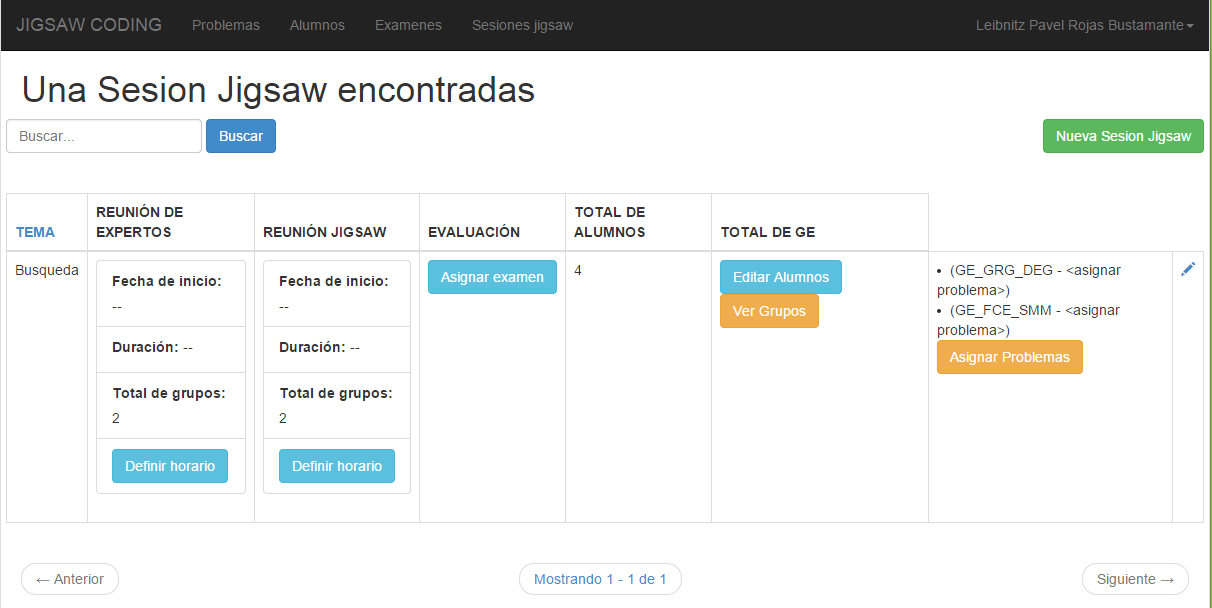
\includegraphics[scale=0.5]{figuras/usodelsistema/docente/sesionesjigsaw_nuevo_06}}
	\end{figure}
	\item Luego de haber generado los grupos, presione el botón Asignar Problemas para indicar qué problema debe resolver cada grupo experto. \autoref{fig:sesionesjigsaw_nuevo_07}
	\begin{figure}
		\centering
		\caption{Sistema Jigsaw Coding - Nueva sesión jigsaw}
		\label{fig:sesionesjigsaw_nuevo_07}
		\fbox{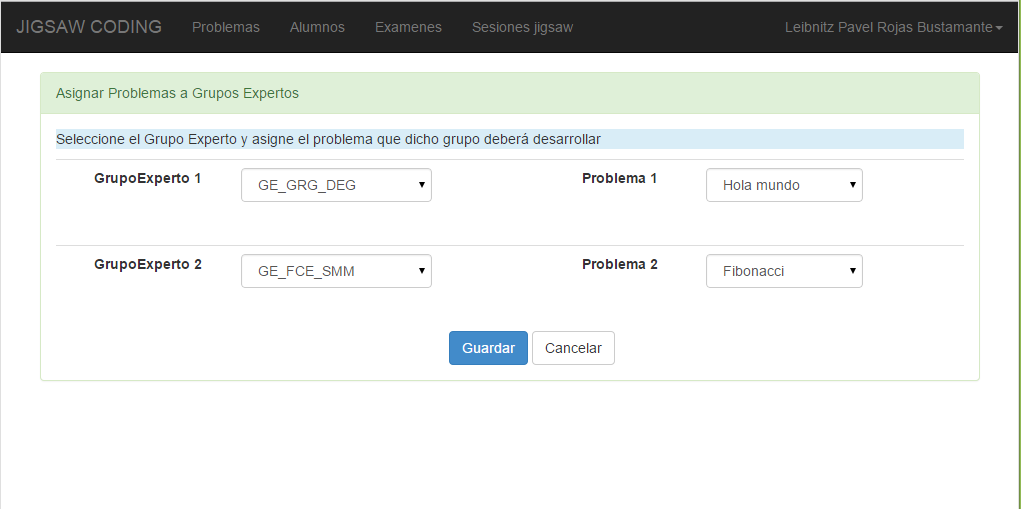
\includegraphics[scale=0.5]{figuras/usodelsistema/docente/sesionesjigsaw_nuevo_07}}
	\end{figure}
	\item Presione el botón Guardar luego de haber asignado a todos los grupos expertos su respectivo problema. El sistema lo redirigirá hacia el panel principal de sesiones jigsaw. \autoref{fig:sesionesjigsaw_nuevo_08}
	\begin{figure}
		\centering
		\caption{Sistema Jigsaw Coding - Nueva sesión jigsaw}
		\label{fig:sesionesjigsaw_nuevo_08}
		\fbox{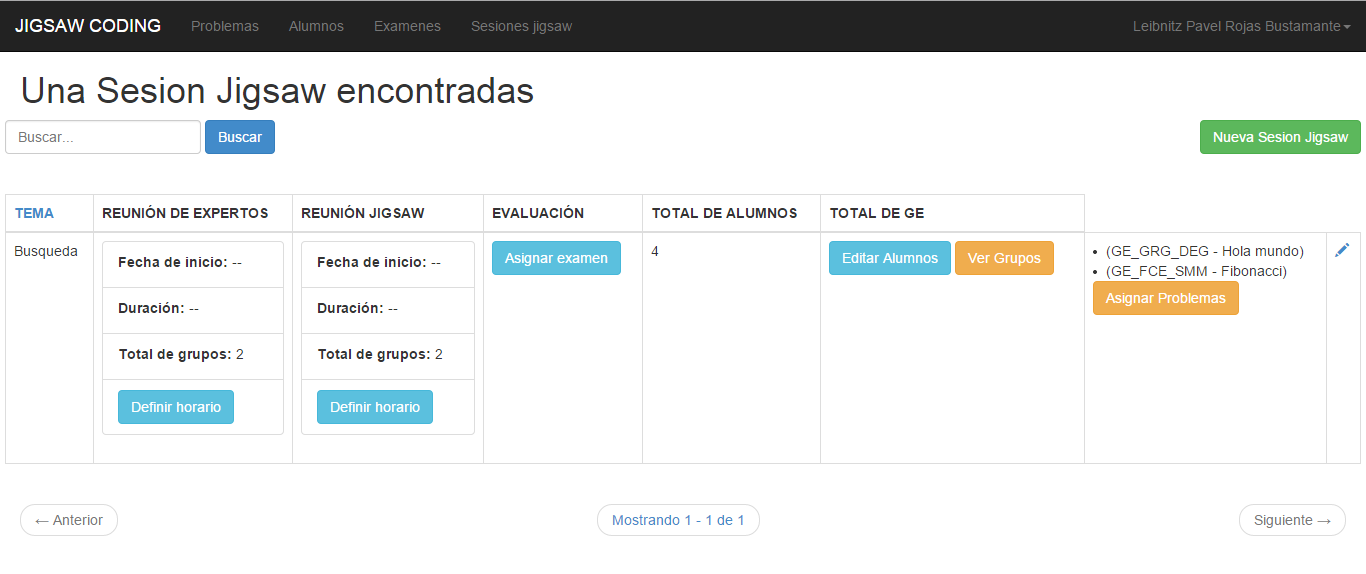
\includegraphics[scale=0.4]{figuras/usodelsistema/docente/sesionesjigsaw_nuevo_08}}
	\end{figure}
	\item Para la fase de evaluación, presione el botón Asignar Examen para seleccionar el examen que será incluído en la sesión jigsaw. \autoref{fig:sesionesjigsaw_nuevo_09}
	\begin{figure}
		\centering
		\caption{Sistema Jigsaw Coding - Asignar examen a sesión jigsaw}
		\label{fig:sesionesjigsaw_nuevo_09}
		\fbox{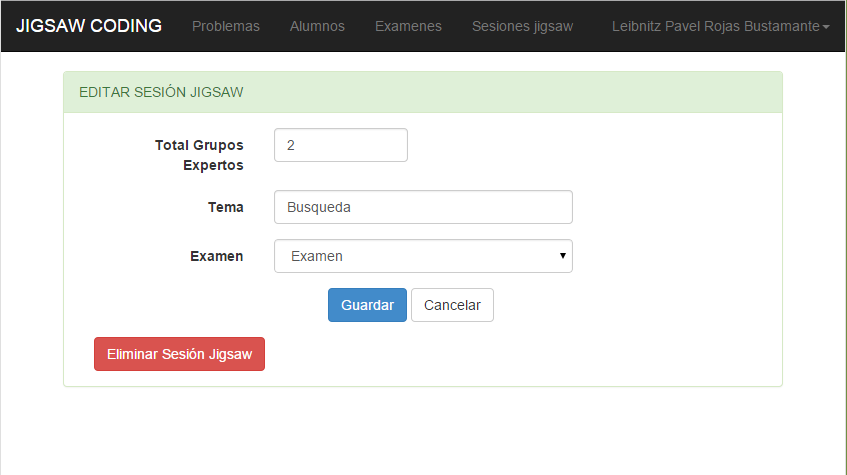
\includegraphics[scale=0.5]{figuras/usodelsistema/docente/sesionesjigsaw_nuevo_09}}
	\end{figure}
	\item Presione el botón Definir Horario para establecer la fecha y hora de inicio para la reunión de expertos, así como también la duración de la misma. \autoref{fig:sesionesjigsaw_nuevo_11}
	\begin{figure}
		\centering
		\caption{Sistema Jigsaw Coding - Definir horario de reunión de expertos}
		\label{fig:sesionesjigsaw_nuevo_11}
		\fbox{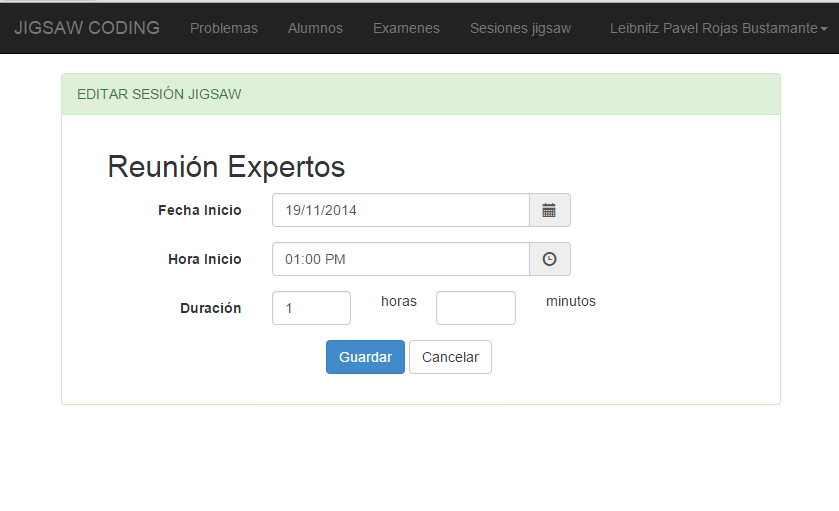
\includegraphics[scale=0.5]{figuras/usodelsistema/docente/sesionesjigsaw_nuevo_11}}
	\end{figure}
	\item Presione el botón Definir Horario para establecer la fecha y hora de inicio para la reunión jigsaw, así como también la duración de la misma. \autoref{fig:sesionesjigsaw_nuevo_13}
	\begin{figure}
		\centering
		\caption{Sistema Jigsaw Coding - Definir horario de reunión jigsaw}
		\label{fig:sesionesjigsaw_nuevo_13}
		\fbox{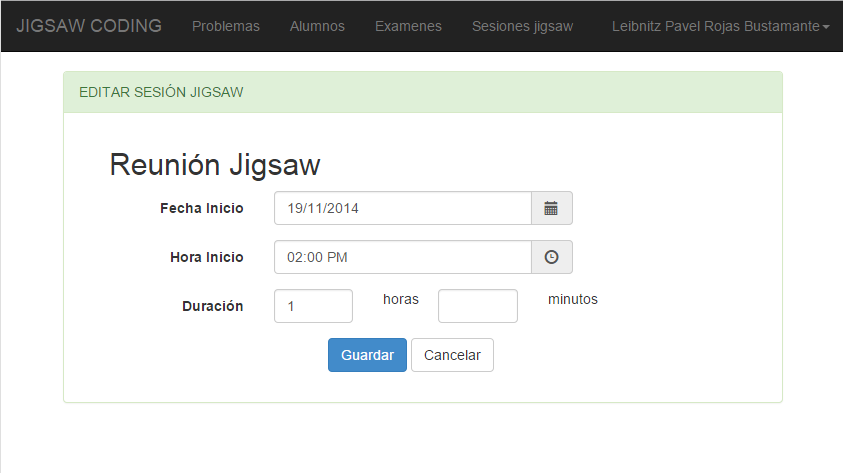
\includegraphics[scale=0.5]{figuras/usodelsistema/docente/sesionesjigsaw_nuevo_13}}
	\end{figure}
	\item Presione el botón Definir Horario para establecere la fecha y hora de inicio para la evaluación, así como también la duración de la misma. \autoref{fig:sesionesjigsaw_nuevo_15}
	\begin{figure}[h]
		\centering
		\caption{Sistema Jigsaw Coding - Definir horario de examen}
		\label{fig:sesionesjigsaw_nuevo_15}
		\fbox{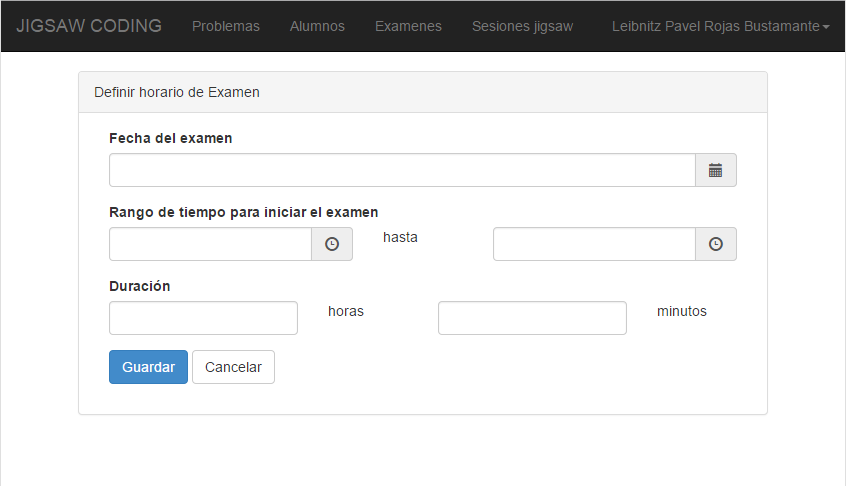
\includegraphics[scale=0.5]{figuras/usodelsistema/docente/sesionesjigsaw_nuevo_15}}
	\end{figure}
\end{enumerate}

\subsection{Unirse a reunión de expertos}
Para que un usuario con perfil Alumno pueda unirse a una reunión de expertos, debe seguir los siguientes pasos:

\begin{enumerate}
	\item Inicie sesión en el Sistema Jigsaw Coding. Si el logueo se realiza exitosamente, entonces, en la pantalla principal del perfil alumno se motrará el listado de sesiones jigsaw a las cuales el alumno puede tener acceso. \autoref{fig:c4_alumno_principal}
	
	\begin{figure}
		\centering
		\caption{Sistema Jigsaw Coding - Perfil alumno}
		\label{fig:c4_alumno_principal}
		\fbox{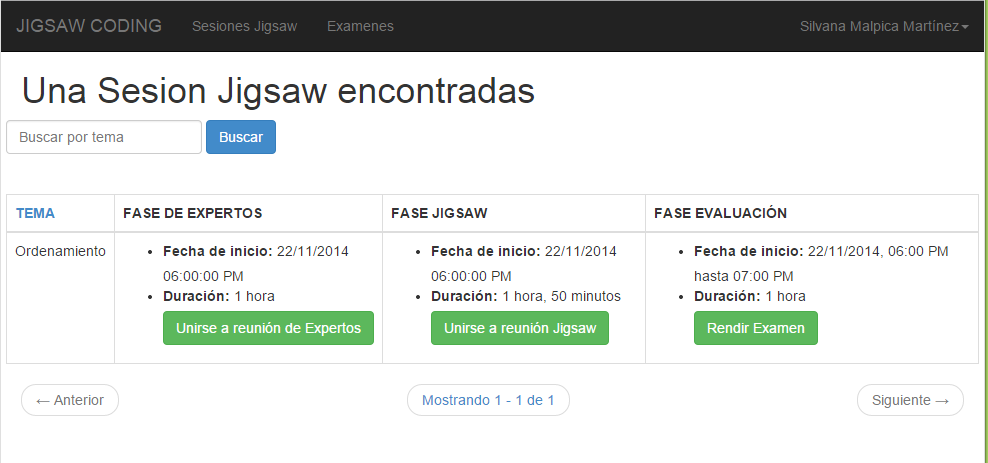
\includegraphics[scale=0.5]{figuras/usodelsistema/alumno/principal}}
	\end{figure}
	
	\item Presione el botón \textbf{Unirse a reunión de Expertos}. A continuación el sistema le mostrará el panel de la reunión de expertos. 
	
	\begin{figure}
		\centering
		\caption{Sistema Jigsaw Coding - Unirse a reunión de expertos}
		\label{fig:c4_reunion_expertos}
		\fbox{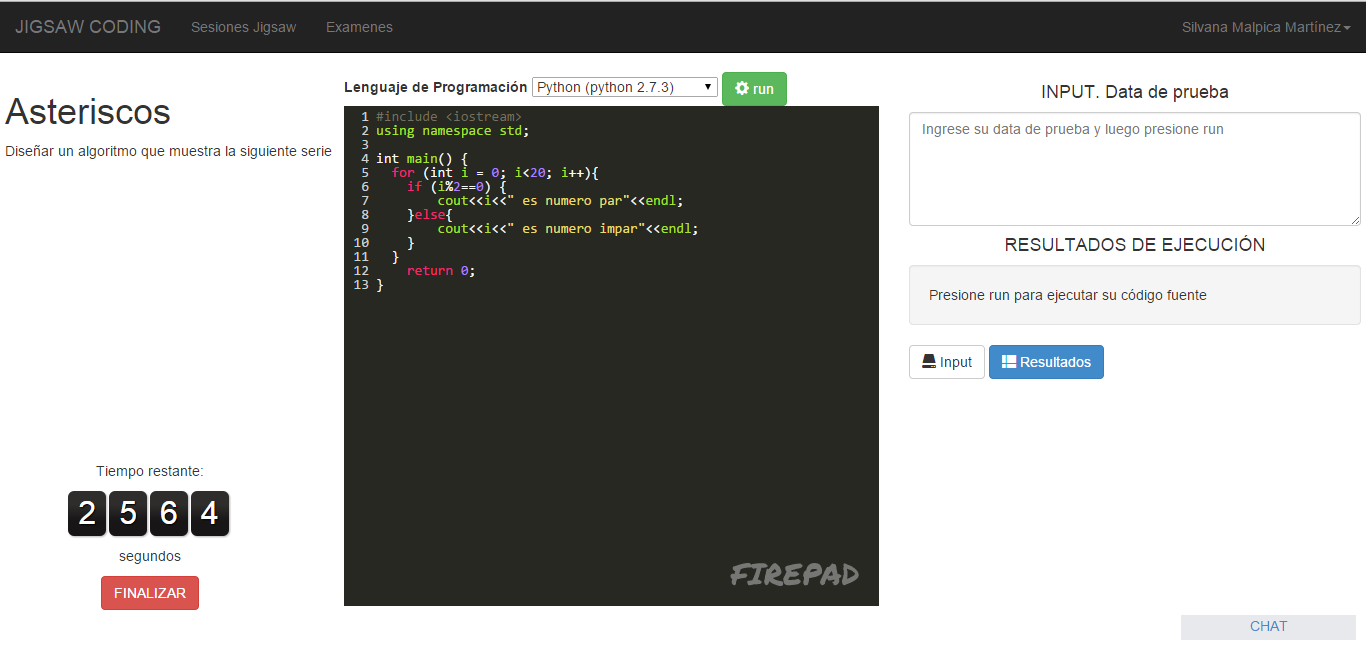
\includegraphics[scale=0.4]{figuras/usodelsistema/alumno/reunion_expertos}}
	\end{figure}
	
	En el panel de reunión de expertos (\autoref{fig:c4_reunion_expertos}) se encontrará lo siguiente: 

	\begin{itemize}
		\item Enunciado del problema.
		\item Editor colaborativo de código fuente.
		\item Menú desplegable para seleccionar el lenguaje de programación(Python, C++ o Java).
		\item Cuadro de texto para ingresar datos de prueba.
		\item Panel de resultados de ejecución.
		\item Chat para comunicarse con el resto de integrantes del grupo experto.
		\item Reloj que marca los segundos restantes para finalizar la reunión de expertos.
	\end{itemize}
\end{enumerate}


\subsection{Unirse a reunión jigsaw}
Para que un usuario con perfil Alumno pueda unirse a una reunión jigsaw, debe seguir los siguientes pasos:

\begin{enumerate}
	\item Inicie sesión en el Sistema Jigsaw Coding. Si el logueo se realiza exitosamente, entonces, en la pantalla principal del perfil alumno se motrará el listado de sesiones jigsaw a las cuales el alumno puede tener acceso.\autoref{fig:c4_alumno_principal}
	\item Presione el botón \textbf{Unirse a reunión Jigsaw}. A continuación el sistema le mostrará el panel de la reunión jigsaw. 
	
	\begin{figure}
		\centering
		\caption{Sistema Jigsaw Coding - Unirse a reunión jigsaw}
		\label{fig:c4_reunion_jigsaw}
		\fbox{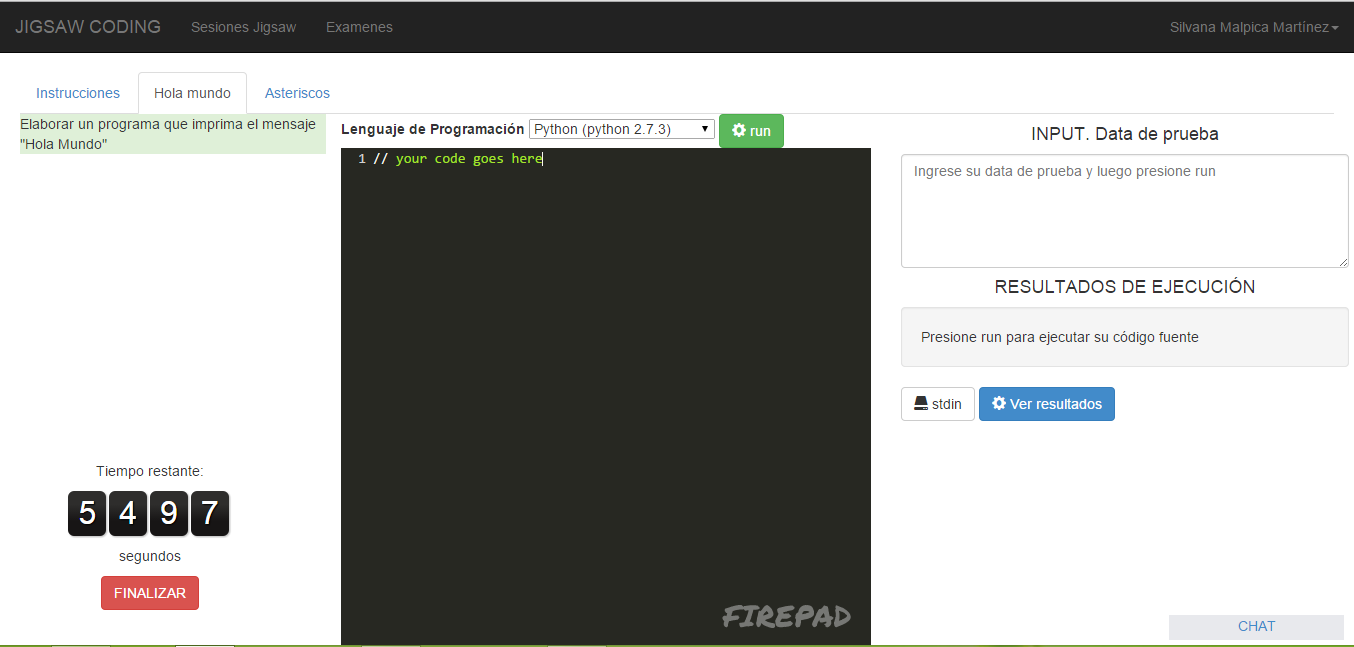
\includegraphics[scale=0.4]{figuras/usodelsistema/alumno/reunion_jigsaw}}
	\end{figure}
	
	En el panel de reunión jigsaw  (\autoref{fig:c4_reunion_jigsaw}) se encontrará lo siguiente: 
	
	\begin{itemize}
		\item Una pestaña con instrucciones que los miembros del grupos jigsaw deben tener en cuenta durante la reunión jigsaw.
		\item Una pestaña por cada problema que el grupo debe resolver.
		\item Enunciado de cada uno de los problemas.
		\item Editor colaborativo de código fuente para cada problema.
		\item Menú desplegable para seleccionar el lenguaje de programación(Python, C++ o Java).
		\item Cuadro de texto para ingresar datos de prueba para cada problema.
		\item Panel de resultados de ejecución para cada problema.
		\item Chat para comunicarse con el resto de integrantes del grupo jigsaw.
		\item Reloj que marca los segundos restantes para finalizar la reunión jigsaw.
	\end{itemize}
\end{enumerate}

\subsection{Rendir evaluación}
Para que un usuario con perfil Alumno pueda rendir un examen, debe seguir los siguientes pasos:

\begin{enumerate}
	\item Inicie sesión en el Sistema Jigsaw Coding. Si el logueo se realiza exitosamente, entonces, en la pantalla principal del perfil alumno se motrará el listado de sesiones jigsaw a las cuales el alumno puede tener acceso.\autoref{fig:c4_alumno_principal}
	\item Presione el botón \textbf{Rendir Examen}. A continuación el sistema le mostrará el panel del examen.
	
	\begin{figure}
		\centering
		\caption{Sistema Jigsaw Coding - Rendir examen}
		\label{fig:c4_rendir_examen}
		\fbox{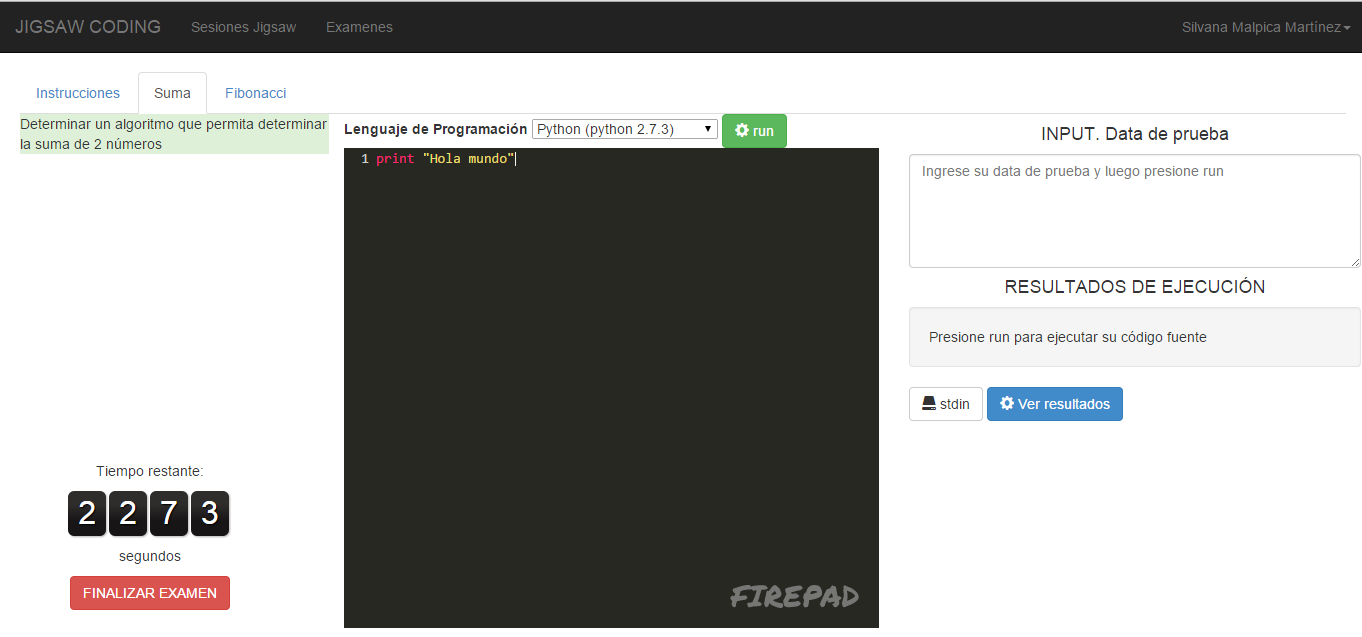
\includegraphics[scale=0.4]{figuras/usodelsistema/alumno/rendir_examen}}
	\end{figure}
	
	En el panel de examen  (\autoref{fig:c4_rendir_examen}) se encontrará lo siguiente: 
	
	\begin{itemize}
		\item Una pestaña con instrucciones que el alumno deben tener en cuenta durante el examen.
		\item Una pestaña por cada problema que el alumno debe resolver.
		\item Enunciado de cada uno de los problemas.
		\item Editor de código fuente para cada problema.
		\item Menú desplegable para seleccionar el lenguaje de programación(Python, C++ o Java).
		\item Cuadro de texto para ingresar datos de prueba para cada problema.
		\item Panel de resultados de ejecución para cada problema.
		\item Reloj que marca los segundos restantes para finalizar el examen.
	\end{itemize}
	
	\item Luego de rendir el examen, el alumno debe esperar a que el docente califique sus respuestas y le asigne una nota, la cual podrá ser vista en el menú \textbf{Examenes}. \autoref{fig:c4_nota_de_examen}
	
	\begin{figure}[!h]
		\centering
		\caption{Sistema Jigsaw Coding - Ver nota de examen}
		\label{fig:c4_nota_de_examen}
		\fbox{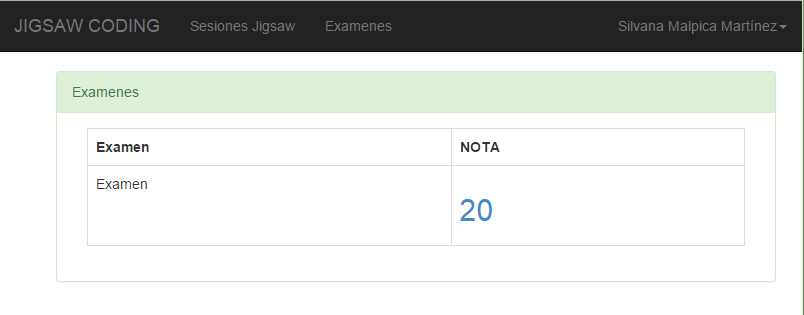
\includegraphics[scale=0.3]{figuras/usodelsistema/alumno/nota_de_examen}}
	\end{figure}
	
\end{enumerate}
\clearpage
\section{Definición de métricas de calidad para el Sistema Jigsaw Coding}
\label{sec:metricas_calidad}
A continuación se presentan las métricas de calidad que se medirán en Sistema Jigsaw Coding, las cuales están basadas en la norma ISO-9126 que establece un estándar internacional para la evaluación de la calidad de los productos software. \cite{iso9126-3}.

\subsection{Entendibilidad}
La presente métrica se refiere a la característica de \textit{Usabilidad} , donde se medirá el grado de \textit{Entendibilidad} que tiene el Sistema para los usuarios. \autoref{tab:c4_entendibilidad}
\begin{longtable}{L{4cm}L{8cm}}
	\caption{Métrica de calidad: Entendibilidad}
	\label{tab:c4_entendibilidad}\\
	\toprule[0.8mm]
	\textbf{Nombre} & \textbf{Entendibilidad del Sistema}\\
	\midrule
	Código & MC-\metrica\\
	\midrule
	Característica & Usabilidad \\
	\midrule
	Sub-característica & Entendibilidad\\
	\midrule
	Propósito & ¿Qué porcentaje de los usuarios consideran que las funcionalidades del sistema son fáciles o muy fáciles de entender? \\
	\midrule
	Método de aplicación & ¿Qué tan fácil o difícil le resultó entender las funcionalidades del sistema?
	\begin{itemize}
		\item Muy fácil
		\item Fácil
		\item Ni fácil ni difícil
		\item Difícil
		\item Muy difícil
	\end{itemize}\\
	\midrule
	\multirow{3}{*}{ \parbox{4cm}{ Medición, fórmula y elementos medibles}   } & $$x = \frac{A}{B} $$\\
	& A : Cantidad de usuarios que selecionaron la alternativa Fácil o Muy fácil.\\
	& B : Cantidad de usuarios encuestados.	\\
	\midrule
	Tipo de medida & A,B: contador \\
	\midrule
	Interpretación del valor & Lo más cercano a 1 es mejor \\
	\midrule
	Tipo de escala & Absoluta \\
	\bottomrule[0.8mm]	
\end{longtable}




%\subsection{Adecuación}
%Esta métrica se refiere a la característica de \textit{Funcionalidad} , donde se medirá el nivel de \textit{Adecuación} que tiene el Sistema Jigsaw Coding. \autoref{tab:c4_adecuacion}
%\begin{longtable}{L{4cm}L{8cm}}
%	\caption{Métrica de calidad: Adecuación}
%	\label{tab:c4_adecuacion}\\
%	\toprule[0.8mm]
%	\textbf{Nombre de la métrica} & \textbf{Adecuación del Sistema Jigsaw Coding}\\
%	\midrule
%	Código & MC-\metrica\\
%	\midrule
%	Característica &  Funcionalidad\\
%	\midrule
%	Sub-característica & Adecuación\\
%	\midrule
%	Propósito &  ¿Qué cantidad de casos de uso no se encuentran dentro de las funcionalidades del sistema jigsaw coding?\\
%	\midrule
%	Método de aplicación & Contar el total de casos de uso que no se pueden realizar a través del sistema jigsaw coding\\
%	\midrule
%	\multirow{3}{*}{ \parbox{4cm}{ Medición, fórmula y elementos medibles}   } & $$x = \frac{A}{B} $$\\
%	& A : Cantidad de casos de uso implementados en el sistema.\\
%	& B : Cantidad de casos de uso especificados en el \autoref{apendice.A}	\\
%	\midrule
%	Tipo de medida & A,B: Contador \\
%	\midrule
%	Interpretación del valor &  Lo más cercano a 1 es mejor\\
%	\midrule
%	Tipo de escala & Absoluta \\
%	\bottomrule[0.8mm]
%\end{longtable}

\subsection{Portabilidad}
La presente métrica se refiere a la característica de \textit{Portabilidad} , en la que se medirá el grado de \textit{Adaptabilidad} que tiene el Sistema desarrollado. \autoref{tab:c4_portabilidad}
\begin{longtable}{L{4cm}L{8cm}}
	\caption{Métrica de calidad: Portabilidad}
	\label{tab:c4_portabilidad}\\
	\toprule[0.8mm]
	\textbf{Nombre de la métrica} & \textbf{Portabilidad del Sistema Jigsaw Coding}\\
	\midrule
	Código & MC-\metrica\\
	\midrule
	Característica & Portabilidad \\
	\midrule
	Sub-característica & Adaptabilidad\\
	\midrule
	Propósito &  ¿En cuántos navegadores web puede usarse el sistema sin tener problemas?\\
	\midrule
	Método de aplicación & Utilizar el sistema en diversos navegarores y contar en cuántos de ellos el sistema funciona correctamente.\\
	\midrule
	\multirow{2}{*}{ \parbox{4cm}{ Medición, fórmula y elementos medibles}   } & $$x = n $$\\
	& n : Número de navegadores web en los que el sistema funciona correctamente.\\
	\midrule
	Tipo de medida &  n: Contador\\
	\midrule
	Interpretación del valor &  A mayor valor de $x$ mejor.\\
	\midrule
	Tipo de escala &  Absoluta\\
	\bottomrule[0.8mm]
\end{longtable}

\clearpage
\subsection{Eficiencia}
La presente métrica se refiere a la característica de \textit{Eficiencia} , donde se medirá el \textit{Tiempo de respuesta} que tiene el Sistema. \autoref{tab:c4_eficiencia}.
\begin{longtable}{L{4cm}L{8cm}}
	\caption{Métrica de calidad: Eficiencia}
	\label{tab:c4_eficiencia}\\
	\toprule[0.8mm]
	\textbf{Nombre de la métrica} & \textbf{Eficiencia del Sistema Jigsaw Coding}\\
	\midrule
	Código & MC-\metrica\\
	\midrule
	Característica & Eficiencia \\
	\midrule
	Sub-característica & Tiempo de respuesta\\
	\midrule
	Propósito & ¿Cuál es el promedio de tiempo de respuesta del Sistema Jigsaw Coding? \\
	\midrule
	Método de aplicación & Medir el tiempo de respuesta de las funcionalidades más importantes del sistema: Generar grupos, Unirse a Reunión de Expertos, Unirse a Reunión Jigsaw, Rendir Examen, Resolver problema(Compilar).\\
	\midrule
	\multirow{2}{*}{ \parbox{4cm}{ Medición, fórmula y elementos medibles}   } 
	& $$x = \sum_{i}^{n}{t_{i}} $$\\
	& $t_{i}$ : Tiempo de respuesta en milisegundos de la funcionalidad $i$.\\
	\midrule
	Tipo de medida & $t_{i}$: milisegundos \\
	\midrule
	Interpretación del valor & Lo más cercano a 0 es mejor \\
	\midrule
	Tipo de escala & Absoluta \\
	\bottomrule[0.8mm]	
\end{longtable}

%\begin{longtable}{L{4cm}L{8cm}}
%	\toprule[0.8mm]
%	\textbf{Nombre de la métrica} & \textbf{}\\
%	\midrule
%	Código & MC-\metrica\\
%	\midrule
%	Característica &  \\
%	\midrule
%	Sub-característica & \\
%	\midrule
%	Propósito &  \\
%	\midrule
%	Método de aplicación &\\
%	\midrule
%	Medición, fórmula y elementos medibles
%	& 	\\
%	\midrule
%	Tipo de medida &  \\
%	\midrule
%	Interpretación del valor &  \\
%	\midrule
%	Tipo de escala &  \\
%	\bottomrule[0.8mm]
%\end{longtable}











































\appendix
\chapter{Casos de Uso}\label{apendice.A}
\section{Introducción}
\subsection{Propósito}
El propósito de este documento es describir de una forma clara y concreta cada uno de los casos de uso definidos para el sistema web a implementar.
\subsection{Alcance}
Los casos de uso presentados en este documento representan los requerimientos que se desean implementar en el sistema web para el aprendizaje colaborativo.
\subsection{Definiciones, acrónimos y abreviaciones}
\begin{enumerate}
  \item CU: Caso de uso
  \item SAC: Sistema para el aprendizaje colaborativo
\end{enumerate}
\clearpage
\section{Catálogo de actores}
En la  \autoref{fig:actores} se puede ver los actores que participan en el Sistema Jigsaw Coding y en la \autoref{tab:actores} se encuentra una breve descripción de cada uno de ellos.
\begin{figure}
  \centering
  % Requires \usepackage{graphicx}
  \fbox{\includegraphics[scale=0.6]{figuras/casosdeuso/actores.jpg}}\\
  \caption[Diagrama de actores]{Diagrama de actores}
  \label{fig:actores}
\end{figure}

\begin{longtable}{L{3cm}L{7cm}}
\caption{Actores}
\label{tab:actores}\\
    \toprule[0.8mm]
    ACTOR & DESCRIPCIÓN \\
    \midrule[0.6mm]
    Usuario & Persona que usará el sistema web de tiempo real para el aprendizaje colaborativo.\\
    \midrule
    Docente & Es la persona responsable de crear y dirigir las sesiones de clase que serán aplicadas a los alumnos. Además, el docente es el responsable de las evaluaciones que rendirán los alumnos una vez terminada cada sesión de clase.\\
    \midrule
    Alumno & Es la persona que será instruida en temas de algoritmos y programación a través de cada sesión diseñada por el docente.\\
    \bottomrule[0.8mm]
\end{longtable}
\clearpage
\begin{landscape}
\section{Diagramas de casos de uso}
\subsection{Casos de uso}
\begin{figure}[!h]
  \centering
  % Requires \usepackage{graphicx}
  \fbox{\includegraphics[scale=0.4]{figuras/casosdeuso/casos_de_uso.jpg}}\\
  \caption[Casos de uso]{Diagrama de casos de uso para el sistema JigsawCoding}
  \label{fig:casos_de_uso}
\end{figure}
\end{landscape}
\clearpage

\section{Especificaciones de Casos de Uso}

\subsection{Iniciar sesión}
\begin{longtable}{|c|L{10cm}|}
	\toprule[0.8mm]
	Código &  CUS-\casodeuso\\  \midrule
	Nombre &  INICIAR SESIÓN.\\  \midrule
	Descripción & El caso de uso describe los pasos para acceder al Sistema Jigsaw Coding.\\  \midrule
	Actores & Docente, Alumno. \\  \midrule
	Precondiciones &  Ninguna.\\  \midrule
	Postcondiciones &  Ninguna.\\  \midrule
	Flujo básico &  \begin{enumerate}
		\item El docente o alumno escribe su correo electrónico como usuario.
		\item El docente o alumno escribe su Password.
		\item El docente o alumno presiona el botón Ingresar.
	\end{enumerate}
	\\  \midrule
	Flujo alternativo &  Ninguno.\\  \bottomrule[0.8mm]
\end{longtable}
\clearpage
\subsection{Registrar Alumno}
\begin{longtable}{|c|L{10cm}|}
  \toprule[0.8mm]
  % after \\: \midrule or \cline{col1-col2} \cline{col3-col4} ...
  Código &  CUS-\casodeuso\\  \midrule
  Nombre &  REGISTRAR ALUMNO.\\  \midrule
  Descripción & El caso de uso inicia cuando el docente selecciona la opción registrar nuevo alumno. Luego completa la información del alumno y el caso de uso termina cuando se presiona la opción Guardar. \\  \midrule
  Actores & Docente. \\  \midrule
  Precondiciones &  El docente debe estar logueado en el sistema.\\  \midrule
  Postcondiciones &  Ninguna.\\  \midrule
  Flujo básico &  \begin{enumerate}
                    \item El docente selecciona la opción para registrar un nuevo alumno.
                    \item El sistema muestra el formulario para completar los datos del alumno.
                    \item El docente completa los campos DNI, Apellido Paterno, Apellido Materno, Nombres, Email, Sexo, Email, Contraseña, Repetir Contraseña.
                    \item El sistema valida el formato del DNI, apellidos, nombres, email.
                    \item El sistema valida que el email no esté registrado en el sistema.
                    \item El sistema verifica que los campos contraseña y repetir contraseña sean idénticos.
                    \item El sistema registra al nuevo alumno en el sistema.
                  \end{enumerate}
  \\  \midrule
  Flujo alternativo &  Ninguno.\\  \bottomrule[0.8mm]
\end{longtable}
\clearpage
\subsection{Crear Problema}

%\begin{tabular}{|c|L{9cm}|}
%  \midrule
%  % after \\: \midrule or \cline{col1-col2} \cline{col3-col4} ...
%  Código &  CUS-\casodeuso\\  \midrule
%  Nombre &  \\  \midrule
%  Descripción &  \\  \midrule
%  Actores &  \\  \midrule
%  Precondiciones &  \\  \midrule
%  Postcondiciones &  \\  \midrule
%  Flujo básico &  \\  \midrule
%  Flujo alternativo &  \\  \midrule
%\end{tabular}

\begin{longtable}{|c|L{9cm}|}
  \toprule[0.8mm]
  % after \\: \midrule or \cline{col1-col2} \cline{col3-col4} ...
  Código & CUS-\casodeuso \\  \midrule
  Nombre & CREAR PROBLEMA. \\  \midrule
  Descripción & El caso de uso inicia cuando el usuario accede al sistema y elige la opción crear problema. Luego el usuario redacta el enunciado y demás observaciones sobre el problema y finaliza el caso de uso. \\  \midrule
  Actores & Docente. \\  \midrule
  Precondiciones & El usuario de ser un Docente y estar logueado en el sistema. \\  \midrule
  Postcondiciones & El docente verá en la lista de problemas el problema recién creado. \\  \midrule
  Flujo básico & \begin{enumerate}
                   \item El docente elige la opción NUEVO PROBLEMA.
                   \item El sistema solicita al docente ingresar el título y enunciado del problema.
                   \item El docente escribe el título y enunciado del problema.
                   \item El docente selecciona la opción GUARDAR.
                   \item El sistema guarda el nuevo problema.
                 \end{enumerate}    \\  \midrule
  Flujo alternativo & Ninguno. \\  \bottomrule[0.8mm]
\end{longtable}
\clearpage
\subsection{Crear sesión jigsaw}
\begin{longtable}{|c|L{10cm}|}
  \toprule[0.8mm]
  % after \\: \midrule or \cline{col1-col2} \cline{col3-col4} ...
  Código &  CUS-\casodeuso\\  \midrule
  Nombre &  CREAR SESIÓN JIGSAW.\\  \midrule
  Descripción &  El caso de uso inicia cuando el usuario accede al sistema y elige la opción de crear una nueva sesión de clase jigsaw; luego ingresa los datos necesarios de la sesión de clase y el caso de uso termina cuando la nueva sesión es creada satisfactoriamente en el sistema.\\  \midrule
  Actores &  Docente.\\  \midrule
  Precondiciones & El usuario debe ser un Docente y estar logueado en el sistema. Los grupos expertos deben haber sido creados. \\  \midrule
  Postcondiciones & El docente verá en el listado de clases la nueva sesión creada. \\  \midrule
  Flujo básico & \begin{enumerate}
                    \item El docente abre un formulario para crear una nueva sesión de clase jigsaw.
                    \item El docente rellena el campo tema.                    
                    \item El docente indica el número total de grupos expertos a incluir en la sesión.
                    \item El docente selecciona la opción Guardar.
                    \item El sistema graba la información de la nueva sesión jigsaw.
                 \end{enumerate}
   \\  \midrule
  Flujo alternativo & Ninguno. \\  \bottomrule[0.8mm]
\end{longtable}
\clearpage
\subsection{Modificar sesión jigsaw}
\begin{longtable}{|c|L{10cm}|}
  \toprule[0.8mm]
  % after \\: \midrule or \cline{col1-col2} \cline{col3-col4} ...
  Código &  CUS-\casodeuso\\  \midrule
  Nombre &  MODIFICAR SESIÓN JIGSAW\\  \midrule
  Descripción & El caso de uso inicia cuando el usuario accede al sistema y selecciona la opción modificar sesión jigsaw. El usuario realiza los cambios que requiera y luego finaliza el caso de uso. \\  \midrule
  Actores &  Docente.\\  \midrule
  Precondiciones &  El usuario debe ser un Docente y debe estar logueado en el sistema. Debe existir una sesión jigsaw en el sistema.\\  \midrule
  Postcondiciones &  Ninguna.\\  \midrule
  Flujo básico & \begin{enumerate}
                    \item El docente selecciona una sesión jigsaw creada y luego elige la opción editar.
                    \item El docente puede cambiar el total de grupos expertos y el tema o examen de la sesión jigsaw.
                    \item El docente selecciona la opción FINALIZAR.
                    \item El sistema guarda los cambios realizados a la sesión jigsaw.

                 \end{enumerate}
   \\  \bottomrule[0.8mm]
  Flujo alternativo &  Ninguno.\\  \midrule
\end{longtable}
\clearpage
\subsection{Asignar alumnos a sesión jigsaw}
\begin{longtable}{|c|L{10cm}|}
	\toprule[0.8mm]
	% after \\: \midrule or \cline{col1-col2} \cline{col3-col4} ...
	Código &  CUS-\casodeuso\\  \midrule
	Nombre &  ASIGNAR ALUMNOS A SESIÓN JIGSAW\\  \midrule
	Descripción &  El caso de uso inicia cuando el docente selecciona la opción Asignar Alumnos para un determinada sesión jigsaw, luego agrega a los alumnos y cuando presiona la opción guardar, el caso de uso termina.\\  \midrule
	Actores &  Docente.\\  \midrule
	Precondiciones &  El usuario de ser un Docente y estar logueado en el sistema. Deben existir alumnos registrados.\\  \midrule
	Postcondiciones &  Ninguna.\\  \midrule
	Flujo básico &    \begin{enumerate}
		\item El docente selecciona la opción Asignar Alumnos en la lista de sesiones jigsaw.
		\item El docente arrastra a los alumnos desde la lista de disponibles hacia la lista de alumnos para la sesión jigsaw.
		\item El docente presiona la opción Guardar.
		\item El sistema guarda la lista de participantes de la sesión jigsaw.
	\end{enumerate}  \\ \midrule
	Flujo alternativo & Ninguno. \\  \bottomrule[0.8mm]
\end{longtable}
\clearpage
\subsection{Generar grupos}
\begin{longtable}{|c|L{10cm}|}
	\toprule[0.8mm]
	% after \\: \midrule or \cline{col1-col2} \cline{col3-col4} ...
	Código &  CUS-\casodeuso\\  \midrule
	Nombre &  GENERAR GRUPOS\\  \midrule
	Descripción &  El caso de uso inicia cuando el docente selecciona la opción Generar Grupos y luego el sistema forma los grupos expertos y grupos jigsaw de forma aleatoria.\\  \midrule
	Actores &  Docente\\  \midrule
	Precondiciones &  El usuario de ser un Docente y estar logueado en el sistema. Deben existir alumnos asignados a una sesión jigsaw.\\  \midrule
	Postcondiciones &  Ninguna.\\  \midrule
	Flujo básico &    \begin{enumerate}
		\item El docente selecciona la opción Generar Grupos.
		\item El sistema genera aleatoriamente los grupos expertos.
		\item El sistema genera aleatoriamente los grupos jigsaw.
		\item El sistema muestra al usuario los grupos creados.
	\end{enumerate}  \\ \midrule
	Flujo alternativo & Ninguno. \\  \bottomrule[0.8mm]
\end{longtable}
\clearpage
\subsection{Asignar problemas a grupos expertos}
\begin{longtable}{|c|L{10cm}|}
	\toprule[0.8mm]
	% after \\: \midrule or \cline{col1-col2} \cline{col3-col4} ...
	Código &  CUS-\casodeuso\\  \midrule
	Nombre &  ASIGNAR PROBLEMAS A GRUPOS EXPERTOS\\  \midrule
	Descripción &  El caso de uso empieza cuando el docente selecciona la opción asignar problemas. Luego indica qué problema debe resolver cada grupo experto y cuando presiona la opción guardar, el caso de uso finaliza.\\  \midrule
	Actores &  Docente.\\  \midrule
	Precondiciones &  El usuario de ser un Docente y estar logueado en el sistema. Los grupos expertos deben haber sido generados por el sistema.\\  \midrule
	Postcondiciones &  Ninguna.\\  \midrule
	Flujo básico &    \begin{enumerate}
		\item El docente selecciona la opción Asignar Problemas.
		\item El docente selecciona un grupo experto y selecciona su respectivo problema.
		\item El docente presiona la opción Guardar.
	\end{enumerate}  \\ \midrule
	Flujo alternativo & Ninguno. \\  \bottomrule[0.8mm]
\end{longtable}
\clearpage
\subsection{Crear examen}
\begin{longtable}{|c|L{10cm}|}
  \toprule[0.8mm]
  % after \\: \midrule or \cline{col1-col2} \cline{col3-col4} ...
  Código &  CUS-\casodeuso\\  \midrule
  Nombre &  CREAR EXAMEN.\\  \midrule
  Descripción & El caso de uso inicia cuando el usuario accede al sistema y elige la opción Nuevo Examen. Luego el usuario selecciona las preguntas o problemas e indica el puntaje de cada una de ellas. El caso de uso termina cuando el usuario selecciona guardar el nuevo examen. \\  \midrule
  Actores &  Docente.\\  \midrule
  Precondiciones & El usuario debe ser un docente y debe estar logueado en el sistema. Deben existir problemas creados. \\  \midrule
  Postcondiciones & El docente podrá ver una nueva evaluación en su listado de examenes. \\  \midrule
  Flujo básico & \begin{enumerate}
                    \item El docente selecciona la opción NUEVO EXAMEN.
                    \item El docente busca los problemas disponibles y arrastra el problema seleccionado hacia el panel de examen.
                    \item El docente presiona la opción Agregar Pregunta.
                    \item El docente establece el puntaje a favor y en contra para el problema seleccionado.
                    \item El docente selecciona la opción FINALIZAR.
                    \item El sistema guarda el examen.
                 \end{enumerate}
   \\  \midrule
  Flujo alternativo & Ninguno \\  \midrule
  Excepciones & [6.1] Si el examen no suma 20 puntos, el sistema indicará al docente que debe seguir ingresando problemas o modificar los puntajes de los problemas ya seleccionados.   \\  \bottomrule[0.8mm]
\end{longtable}

\clearpage
\subsection{Asignar examen}
\begin{longtable}{|c|L{10cm}|}
	\toprule[0.8mm]
	% after \\: \midrule or \cline{col1-col2} \cline{col3-col4} ...
	Código &  CUS-\casodeuso\\  \midrule
	Nombre &  ASIGNAR EXAMEN\\  \midrule
	Descripción &  El caso de uso empieza cuando el docente selecciona la opción asignar examen. Luego indica qué examen deberán resolver los alumnos.\\  \midrule
	Actores &  Docente.\\  \midrule
	Precondiciones &  El usuario de ser un Docente y estar logueado en el sistema y deben existir examenes creados.\\  \midrule
	Postcondiciones &  Ninguna\\  \midrule
	Flujo básico &    \begin{enumerate}
		\item El docente selecciona la opción Asignar Examen.
		\item El docente selecciona un examen.
		\item El docente presiona la opción Guardar.
	\end{enumerate}  \\ \midrule
	Flujo alternativo & Ninguno. \\ \bottomrule[0.8mm]
\end{longtable}

\clearpage
\subsection{Definir horario de reunión de expertos}
\begin{longtable}{|c|L{10cm}|}
	\toprule[0.8mm]
	% after \\: \midrule or \cline{col1-col2} \cline{col3-col4} ...
	Código &  CUS-\casodeuso\\  \midrule
	Nombre &  DEFINIR HORARIO DE REUNIÓN DE EXPERTOS\\  \midrule
	Descripción & El caso de uso inicia cuando el usuario accede al sistema y elige la opción Definir Horario en la lista de sesiones jigsaw dentro del cuadro Reunión de Expertos. Luego el usuario indica la fecha y hora de inicio acceder a la reunión de expertos así como también la duración de la misma. El caso de uso termina cuando el usuario selecciona la opción guardar. \\  \midrule
	Actores &  Docente\\  \midrule
	Precondiciones & El usuario debe ser un docente y debe estar logueado en el sistema. Deben existir sesiones jigsaw. \\  \midrule
	Postcondiciones & El docente podrá ver la fecha, hora de inicio de la reunión de expertos y la duración de la misma. \\  \midrule
	Flujo básico & \begin{enumerate}
		\item El docente selecciona la opción Definir Horario para una reunión de expertos.
		\item El docente ingresa la fecha de inicio.
		\item El docente ingresa la hora de inicio.
		\item El docente ingresa la duración de la reunión de expertos.
		\item El docente selecciona la opción FINALIZAR.
		\item El sistema guarda el horario establecido para la reunión de expertos.
	\end{enumerate}
	\\  \midrule
	Flujo alternativo & Ninguno. \\  \bottomrule[0.8mm]
\end{longtable}
\clearpage
\subsection{Definir horario de reunión jigsaw}
\begin{longtable}{|c|L{10cm}|}
	\toprule[0.8mm]
	% after \\: \midrule or \cline{col1-col2} \cline{col3-col4} ...
	Código &  CUS-\casodeuso\\  \midrule
	Nombre &  DEFINIR HORARIO DE REUNIÓN JIGSAW.\\  \midrule
	Descripción & El caso de uso inicia cuando el usuario accede al sistema y elige la opción Definir Horario en la lista de sesiones jigsaw dentro del cuadro Reunión Jigsaw. Luego el usuario indica la fecha y hora de inicio acceder a la reunión jigsaw así como también la duración de la misma. El caso de uso termina cuando el usuario selecciona la opción guardar. \\  \midrule
	Actores &  Docente.\\  \midrule
	Precondiciones & El usuario debe ser un docente y debe estar logueado en el sistema. Deben existir sesiones jigsaw. \\  \midrule
	Postcondiciones & El docente podrá ver la fecha, hora de inicio de la reunión jigsaw y la duración de la misma. \\  \midrule
	Flujo básico & \begin{enumerate}
		\item El docente selecciona la opción Definir Horario para una reunión jigsaw.
		\item El docente ingresa la fecha de inicio.
		\item El docente ingresa la hora de inicio.
		\item El docente ingresa la duración de la reunión jigsaw.
		\item El docente selecciona la opción FINALIZAR.
		\item El sistema guarda el horario establecido para la reunión jigsaw.
	\end{enumerate}
	\\  \midrule
	Flujo alternativo & Ninguno. \\  \bottomrule[0.8mm]
\end{longtable}
\clearpage
\subsection{Definir horario de examen}
\begin{longtable}{|c|L{10cm}|}
  \toprule[0.8mm]
  % after \\: \midrule or \cline{col1-col2} \cline{col3-col4} ...
  Código &  CUS-\casodeuso\\  \midrule
  Nombre &  DEFINIR HORARIO DE EXAMEN.\\  \midrule
  Descripción & El caso de uso inicia cuando el usuario accede al sistema y elige la opción Definir Horario en la lista de examenes creados. Luego el usuario indica el intervalo de tiempo para ingresar al examen así como también la duración del examen. El caso de uso termina cuando el usuario selecciona la opción guardar. \\  \midrule
  Actores &  Docente\\  \midrule
  Precondiciones & El usuario debe ser un docente y debe estar logueado en el sistema. Deben existir examenes creados. \\  \midrule
  Postcondiciones & El docente podrá ver la fecha, hora de inicio del examen y la duración del mismo en su listado de examenes. \\  \midrule
  Flujo básico & \begin{enumerate}
                    \item El docente selecciona la opción Definir Horario en un examen.
                    \item El docente ingresa la fecha de inicio del examen.
                    \item El docente ingresa la hora de inicio del examen.
                    \item El docente ingresa la fecha límite para acceder al examen.
                    \item El docente ingresa la hora límite para acceder al examen.
                    \item El docente selecciona la opción FINALIZAR.
                    \item El sistema guarda el horario establecido para el examen.
                 \end{enumerate}
   \\  \midrule
  Flujo alternativo & Ninguno. \\  \bottomrule[0.8mm]
\end{longtable}
\clearpage
\subsection{Unirse a reunión de expertos}
\begin{longtable}{|c|L{10cm}|}
  \toprule[0.8mm]
  % after \\: \midrule or \cline{col1-col2} \cline{col3-col4} ...
  Código &  CUS-\casodeuso\\  \midrule
  Nombre & UNIRSE A REUNIÓN DE EXPERTOS. \\  \midrule
  Descripción & El caso de uso inicia cuando el alumno selecciona la opción unirse a reunión de expertos. El alumno dispondrá de un tiempo fijado por el docente para debatir y desarrollar el problema planteado de forma colaborativa con los demás miembros del grupo experto. El caso de uso finaliza cuando culmina el tiempo asignado para la reunión de expertos. \\  \midrule
  Actores & Alumno. \\  \midrule
  Precondiciones & Debe existir una sesión jigsaw creada por el docente y el alumno debe estar logueado en el sistema y ser parte de un grupo experto. \\  \midrule
  Postcondiciones & Ninguna. \\  \midrule
  Flujo básico & \begin{enumerate}
                    \item El alumno selecciona en una de las sesiones jigsaw disponibles la opción Unirse a Reunión de Expertos.
                    \item El sistema mostrará al alumno la información del problema asignado(Título, Enunciado, Tiempo disponible) y un editor de código fuente para el trabajo colaborativo.
                    \item El alumno resuelve el problema.
                    \item El alumno usa el chat grupal para consultar al grupo.
                    \item El sistema finalizará la reunión de expertos cuando el reloj marque 0.
                 \end{enumerate}
   \\  \midrule
  Flujo alternativo & Ninguno. \\  \bottomrule[0.8mm]
\end{longtable}
\clearpage
\subsection{Resolver problema}
\begin{longtable}{|c|L{10cm}|}
  \toprule[0.8mm]
  % after \\: \midrule or \cline{col1-col2} \cline{col3-col4} ...
  Código &  CUS-\casodeuso\\  \midrule
  Nombre &  RESOLVER PROBLEMA.\\  \midrule
  Descripción & El caso de uso inicia cuando el alumno ingresa a una reunión o a un examen en el cual debe desarrollar un problema asignado por el docente. \\  \midrule
  Actores &  Alumno.\\  \midrule
  Precondiciones & El alumno debe haber ingresado a una reunión de expertos o reunión jigsaw. \\  \midrule
  Postcondiciones & Ninguna \\  \midrule
  Flujo básico & \begin{enumerate}
                    \item El alumno escribe la solución al problema en el editor de código fuente.
                    \item El alumno ingresa los datos de prueba en el panel correspondiente.
                    \item El alumno selecciona la opción Compilar para compilar su código fuente. 
                    \item El sistema compila y ejecuta el código del alumno.
                    \item El sistema muestra los resultados de la ejecución.
                 \end{enumerate}
   \\  \midrule
  Flujo alternativo & Ninguno. \\  \bottomrule[0.8mm]
\end{longtable}
\clearpage
\subsection{Consultar al grupo}
\begin{longtable}{|c|L{10cm}|}
  \toprule[0.8mm]
  % after \\: \midrule or \cline{col1-col2} \cline{col3-col4} ...
  Código &  CUS-\casodeuso\\  \midrule
  Nombre &  CONSULTAR AL GRUPO.\\  \midrule
  Descripción & El caso de uso inicia cuando el alumno abre la ventana de chat grupal para hacer alguna consulta. \\  \midrule
  Actores &  Alumno\\  \midrule
  Precondiciones & El alumno debe haber ingresado a una reunión de expertos o reunión jigsaw. \\  \midrule
  Postcondiciones & Ninguna. \\  \midrule
  Flujo básico &  \begin{enumerate}
                    \item El alumno abre la ventana de conversación.
                    \item El alumno escribe y envía su consulta.
                    \item El sistema envía la consulta a los demás miembros del grupo.
                    \item El alumno cierra la ventana de conversación.
                  \end{enumerate}
  \\  \midrule
  Flujo alternativo &  Ninguno.\\  \bottomrule[0.8mm]
\end{longtable}
\clearpage
\subsection{Unirse a reunión jigsaw}
\begin{longtable}{|c|L{10cm}|}
  \toprule[0.8mm]
  % after \\: \midrule or \cline{col1-col2} \cline{col3-col4} ...
  Código &  CUS-\casodeuso\\  \midrule
  Nombre &  UNIRSE A REUNIÓN JIGSAW.\\  \midrule
  Descripción & El caso de uso inicia cuando el alumno selecciona la opción unirse a reunión jigsaw. El alumno dispondrá de un tiempo fijado por el docente para debatir y desarrollar los problemas planteados. El caso de uso finaliza cuando culmina el tiempo asignado para la reunión de jigsaw. \\  \midrule
  Actores &  Alumno.\\  \midrule
  Precondiciones & Debe existir una sesión jigsaw creada por el docente y el alumno debe estar logueado en el sistema y ser parte de un grupo jigsaw. \\  \midrule
  Postcondiciones & Ninguna. \\  \midrule
  Flujo básico &  \begin{enumerate}
                    \item El alumno selecciona en una de las sesiones jigsaw disponibles la opción Unirse a Reunión Jigsaw.
                    \item El sistema mostrará al alumno la información de los problemas a desarrollar(Título, Enunciado, Tiempo disponible) y un editor de código fuente para el trabajo colaborativo.
                    \item El alumno resuelve el problema que le tocó en su grupo experto.
                    \item El alumno usa el chat grupal para consultar al grupo.
                    \item El sistema finalizará la reunión jigsaw cuando el reloj marque 0.
                  \end{enumerate}
  \\ 
  \bottomrule[0.8mm]
\end{longtable}
\clearpage
\subsection{Rendir examen}
\begin{longtable}{|c|L{10cm}|}
  \toprule[0.8mm]
  % after \\: \midrule or \cline{col1-col2} \cline{col3-col4} ...
  Código &  CUS-\casodeuso\\  \midrule
  Nombre &  RENDIR EXAMEN.\\  \midrule
  Descripción & El caso de uso inicia cuando el alumno selecciona la opción rendir examen y el sistema le muestra el examen creado por el docente. El alumno desarrolla las preguntas planteadas en el tiempo asignado y cuando selecciona la opción FINALIZAR, el caso de uso termina. \\  \midrule
  Actores &  Alumno\\  \midrule
  Precondiciones & El alumno debe estar logueado en el sistema y debe tener asignado algún examen. \\  \midrule
  Postcondiciones & Ninguna. \\  \midrule
  Flujo básico & \begin{enumerate}
                    \item El alumno selecciona la opción RENDIR EXAMEN.
                    \item El sistema muestra la información del examen(Instrucciones, Preguntas, tiempo restante para resolver el examen).
                    \item El alumno responde a las preguntas.
                    \item El alumno selecciona la opción finalizar.
                    \item El sistema guarda las respuestas y culmina el examen.
                 \end{enumerate}
   \\  \midrule
  Flujo alternativo & Ninguno. \\  \bottomrule[0.8mm]
\end{longtable} 
\chapter{Especificaciones suplementarias}\label{apendice.B}
\section{Introducción}
El propósito de este documento es definir los requerimientos del Sistema web de aprendizaje colaborativo que no pueden ser capturados vía especificación de casos de uso. Estos requerimientos que en su mayoría corresponden a requerimientos no funcionales serán capturados y clasificados según la norma ISO-9126 que define atributos de calidad para productos software.
\section{Funcionalidad} 
\begin{itemize}
\item El sistema no debe tener errores en la asignación de tiempos para cada reunión.
\item El sistema debe validar correctamente la asignación de alumnos a los grupos expertos.
\item El sistema debe limitar el acceso sólo a usuarios debidamente registrados.
\end{itemize}
\section{Fiabilidad o confiabilidad} 
\begin{itemize}
\item El sistema debe funcionar las 24 horas del día.
\item El sistema debe soportar una concurrencia de hasta al menos 50 usuarios.
\item El sistema debe capturar cualquier error y notificarlo sin tener que dejar de funcionar.
\end{itemize}
\section{Usabilidad} 
\begin{itemize}
\item El sistema debe ser intuitivo para el usuario.
\item El sistema debe permitir al usuario que éste aprenda cómo usarlo sin ninguna ayuda adicional.
\item El sistema debe ser amigable para el usuario en cuanto a interfaz(colores y tonos claros, letras claras y legibles).
\end{itemize}
\section{Eficiencia o Performance} 
\begin{itemize}
\item El tiempo de respuesta del sistema no debe exceder de 2 segundos.
\end{itemize}
\section{Mantenibilidad} 
\begin{itemize}
\item El sistema web debe permitir realizar actividades correctivas o de actualización sin afectar el correcto funcionamiento de sus distintos módulos.
\end{itemize}
\section{Portabilidad} 
\begin{itemize}
\item El sistema debe funcionar en los navegadores Chrome y Mozilla Firefox en sus últimas versiones.
\item El sistema debe ser multiplataforma.
\end{itemize}


\chapter{Documento de Arquitectura de Software}
\section{Introducción}
Este documento brinda una vista general de alto nivel sobre cómo será el desarrollo del sistema JigsawCoding. Se resumirá las tecnologías con las cuales se implementará el sistema así como también se proporcionará una descripción de alto nivel de la arquitectura del sistema.
\subsection{Propósito}
El presente documento de arquitectura de software tiene como finalidad describir el sistema web Jigsaw Coding desde diferentes vistas arquitectónicas, las cuales serán de gran utilidad para el desarrollo de dicho sistema.
\subsection{Alcance} Este documento arquitectónico aplica para describir las características arquitectónicas del sistema web JigsawCoding, las tecnologías que serán usadas en su desarrollo y las principales funcionalidades del sistema.
\subsection{Definiciones, acrónimos y abreviaturas}
En esta sección se provee las definiciones, acrónimos y abreviaturas de términos utilizados en el presente documento a fin de brindar al lector una mejor comprensión del contenido. 
\clearpage
\begin{longtable}{|c|L{8cm}|}
    \hline
  UML & Unified Modeling Language: Lenguaje Unificado de Modelamiento \\ \hline
  CRUD & Create - Read - Update - Delete \\ \hline
  JSON & JavaScript Object Notation: Es un formato ligero para el intercambio de datos \\ \hline
  XML & eXtensible Markup Language: Es un lenguaje de marcas utilizado para almacenar datos en forma legible. \\ \hline
  \emph{sbt} & Herramienta de construcción interactiva \url{http://www.scala-sbt.org} \\ \hline
\end{longtable}
\section{Representación arquitectónica}
El sistema web JigsawCoding, será implementado usando una arquitectura Modelo - Vista - Controlador, la misma que está definida en el framework Play de Java.
\subsection{PlayFramework 2.2.4}
Play es framework open source de Java y Scala que integra componentes y APIs necesarios para el desarrollo moderno de aplicaciones web. Play sigue el patrón de arquitectura Modelo - Vista - Controlador y uno de sus objetivos es optimizar la productividad del desarrollador a través del uso de configuraciones estandarizadas, recompilación automática del código fuente y la visualización de errores directamente en el navegador.\\

A pesar que las aplicaciones de Play están diseñadas para correr en servidores web basados en Jboos Netty, también pueden ser deployadas como archivos WAR para ser distribuidos en la mayoría de servidores de aplicaciones Java EE como Apache Tomcat o GlassFish.

\subsubsection{Componentes y Características de Play}
\begin{itemize}
  \item JBoss Netty para el servidor web.
  \item Ebean como ORM para Java.
  \item Scala para el motor de plantillas.
  \item Recompilación de código automática.
  \item \emph{sbt} para la administración de dependencias.
  \item CRUD: un módulo para simplificar la edición de objetos.
  \item Secure: un módulo para establecer simples autenticaciones de usuarios.
  \item Parsers de JSON y XML.
  \item Una capa de persistencia basada en JPA
\end{itemize}
\clearpage
\section{Vista lógica}
\clearpage
\section{Vista de procesos}
\clearpage
\section{Vista de desarrollo}
La vista de despliegue muestra el sistema desde la perspectiva del programador y se ocupa de la gestión del software a implementar. Esto es, en esta vista se describe cómo estará dividido el sistema JigsaCoding en paquetes y las dependencias que habrá entre ellos.
\begin{figure}[!h]
  \centering
  % Requires \usepackage{graphicx}
  \includegraphics[scale=0.6]{figuras/sad/diagrama_de_paquetes.jpg}\\
  \caption{Diagrama de Paquetes}\label{fig:diagrama_de_paquetes}
\end{figure}
\clearpage
\section{Vista física}
\begin{figure}[!h]
  \centering
  % Requires \usepackage{graphicx}
  \includegraphics[scale=0.5]{figuras/sad/diagrama_de_despliegue.jpg}\\
  \caption{Diagrama de Despliegue}\label{fig:diagrama_de_despliegue}
\end{figure}
\section{Vista de escenarios}
\clearpage
\section{Vista de Datos}
\begin{figure}[!h]
  \centering
  % Requires \usepackage{graphicx}
  \includegraphics[scale=0.6]{figuras/sad/modelo_de_datos.png}\\
  \caption[Modelo de datos]{Modelo de base de datos del sistema JigsawCoding}\label{fig:modelo_de_datos}
\end{figure}
\subsection{MySQL 5.6}
El desarrollo del sistema JigsawCoding se hará usando como motor de base de datos a MySQL en su versión 5.6. Este, es un sistema de gestion de base de datos libre actualmente soportado por Oracle. 


%\bibliographystyle{apalike}
\bibliographystyle{apacite}
\bibliography{referencias}
%\addcontentsline{toc}{chapter}{Referencias}

\end{document}
